% -*- coding: UTF-8 -*-
% hurlex.tex
% hurlex 开发文档

% 我们采用 A4 纸,论文风格
\documentclass[11pt, a4paper]{article}

% 必要的宏包
\usepackage{fontspec, graphicx, titlesec, xunicode, xltxtra, natbib}
\usepackage{indentfirst, listings, xcolor, verbatim, fancyvrb, mdframed}

% 显示中文的名称
\renewcommand{\abstractname}{摘要} 
\renewcommand{\contentsname}{目录} 
\renewcommand{\listfigurename}{插图目录}
\renewcommand{\listtablename}{表格目录}
\renewcommand{\refname}{参考文献}
\renewcommand{\abstractname}{摘要}
\renewcommand{\indexname}{索引}
\renewcommand{\tablename}{表}
\renewcommand{\figurename}{图}
\renewcommand{\lstlistingname}{代码}

% 定义我们的页面样式
\newpagestyle{main}{
	% 字体设置
	\setmainfont{PingFang SC}

	% 使用中文的断行规则
	\XeTeXlinebreaklocale "zh"
	\XeTeXlinebreakskip = 0pt plus 1pt minus 0.1pt

	% 页边距设置
	\usepackage[top = 1.2in, bottom = 1.2in, left = 1.2in, right = 1in]{geometry}

	% 页眉和页脚设置
	\sethead{\small\S\, \thesection\quad\sectiontitle}{}{$\cdot$~\thepage~$\cdot$}
	\setfoot{}{}{}
	\headrule
	%\footrule

	% 设置章节目录深度
	\setcounter{tocdepth}{1}

	% 设置章节标题格式
	\titleformat{\section}{\centering\Large\bfseries}{\S\,\thesection}{1em}{}
	\titleformat{\subsection}{\large\bfseries}{\S\,\thesubsection}{1em}{}
	
	% 段落首行缩进 2 字符
	\setlength{\parindent}{2em}

	% 段间距
	\setlength{\parskip}{0.5\baselineskip}
}

% 设置文档页的样式
\pagestyle{main}

% 嵌入代码格式设置
\lstset{numbers = left, 
	keywordstyle = \color{blue}\bfseries,
	numberstyle = \small\color{black},
	backgroundcolor = \color{lightgray},
	basicstyle=\footnotesize,
	stepnumber = 1,
	showstringspaces=false,
	showspaces = false,
	showtabs = false,
	tabsize = 8,
	breaklines = true,
	extendedchars = false
}

% 修改日期的显示格式
\renewcommand{\today}{\number\year 年\number\month 月\number\day 日}

% 设置文档标题和作者信息
\title{一个基于x86架构的简单内核实现}
\author{hurley}
\date{\today}

% 设置参考文献的格式
\bibliographystyle{plain}

% 文档内容从这里开始
\begin{document}

% 输出标题
\maketitle

% 摘要
\begin{abstract}
这是一篇阐述如何在基于Intel x86架构的IBM PC机及其兼容计算机上构建一个简单的操作系统内核的教程。我们将从裸机出发,逐渐展示构建一个简单的操作系统内核的全过程。你可以跟随着笔者的脚步,慢慢体会一个小内核诞生的整体框架和所有细节,进一步了解操作系统的实现原理和在x86架构上的具体实现。
\end{abstract}

% 换页
\clearpage

% 输出目录
\tableofcontents

% 第1章
% -*- coding: UTF-8 -*-
% hurlex-chapt1.tex
% hurlex 开发文档 第1章内容

\section{项目概述和开发环境配置}

\par 这是一篇阐述如何在基于Intel x86架构的IBM PC机及其兼容计算机上构建一个简单的操作系统内核的教程。\footnote{这篇教程很大程度上来自《JamesM's kernel development tutorials》这篇文档,感谢原作者的辛勤劳动。相比较而言我的工作在很大的程度上只是转述和查证。}
我们将一起来探索x86CPU的保护模式下操作系统内核的编写方法,一起感受一次完整的探索过程。虽然这个小内核和一个具有商业价值的操作系统内核相比较而言依旧相差甚远。但是通过这样的探索,相信我们能充分的理解x86保护模式的运行方式和操作系统的基本原理,而这恰恰是传统的通过阅读书籍的方式难以获得的深刻体验。

\par 言归正传,开始我们的征程吧。什么?你已经迫不及待的打开编辑器准备写代码了?别着急,工欲善其事,必先利其器。我们先来阐述一下开发环境和相关的工具配置。

\subsection{选择工作环境}
\par Windows 和 Linux 之争由来已久,我不想在这篇文档里针对这个问题再费口舌。我们的工作环境也选择Linux,对于Windows用户而言只能说声抱歉了。使用Linux的原因很简单,这里有可以自由使用的一系列的开源软件能很好的协助我们的开发和调试工作,而在Windows下缺乏相应的免费工具\footnote {当然也可能是我学习和工作的环境多是Linux,所以对Windows下的工具所知甚少。另外为了避免读者频繁看到诸如"Windows下如何做,Linux下如何做"的字眼而厌烦,所以就只能牺牲一部分读者的感受了,我在此表示歉意。}
。虽然我的构建环境使用的是Fedora 18,但是这不影响大家对于Linux发行版的选择,因为使用的命令基本上都是相同的。\footnote {差异较大的部分应该是软件安装的包管理器了,这个相信大家应该很熟悉自己所使用的发行版所附带的包管理器了。}

\par 同时,为了避免谈及一些Linux基础的命令和基本的计算机概念,我假定读者们已经对以下列出的知识点有一定的理解和掌握:
\begin{itemize}
	\item 熟悉微机原理和基本的操作系统原理,了解基本的计算机原理概念。
	\item 了解和熟悉Intel x86保护模式下的一些名词和概念,至少需要熟悉Intel 8086.
	\item 熟悉和掌握Linux的常用命令,能在Linux下进行基本的系统程序编写。
	\item 掌握简单的x86汇编语言,能读懂和编写简单的汇编程序(至少能看懂)。
	\item 熟练掌握C语言程序的编写,对C语言中较为复杂的语法有所了解。
	\item 理解和掌握C语言程序编译的过程,了解链接的基本原理。
	\item ……
\end{itemize}

\par 我希望之前的描述没有吓到你。也许你本来满怀热情的准备开始干一场"大事业"的热情被一盆水浇凉了很多。假如你没有被吓到,那么我很高兴。即使你真的被那些条款吓到了也不要紧,学习本来就是一个从无到有的过程,操作系统内核的编写本来就是一个及其复杂和麻烦的过程。尽管我们做的东西甚至只是一个基本原理的演示,但那也是实打实的可以运行在裸机\footnote{这里的"裸机"指没有安装操作系统的计算机。}上的小内核。不过千里之行,始于足下。一时的胆怯会在我们逐渐获得的一点点成就感中丧失殆尽。同时我也会尽量降低这个小内核的难度,给充满热情但相关基础较为薄弱的读者阐述尽可能多的背景资料和原理解析(至少也会给出参考资料的链接)。我相信哪怕你之前的基础再弱,至少也能"照猫画虎"的构建出一个可以在裸机上运行的小内核。

\par 相信这个体验会对你以后的学习生涯带来很多难以估量的好处。当你在学习计算机原理的时候,你对计算机的理解将不再是浅浅的、浮于表面的概括,而是深刻的掌握了机器运行的基本原理。那些看似枯燥的理论和概念在你的眼里将是鲜活且富有生机的。相比较一般的用户只是使用计算机而言,我们却在自己的机器上写出了一个可以运行的操作系统内核。这难道不是一件很酷、很Geek、很好玩的事情吗?

\subsection{选择开发语言}
\par 我们解决了工作环境的问题,接下来是语言的选择了。如果我说是汇编语言的话,恐怕很多读者已经彻底失去了读下去的勇气了。但是没有办法,有的地方确实需要使用汇编语言去实现。但是聪明的读者已经注意到前文提到了C语言,没错,很大程度上的代码使用C语言来实现。所以不用过于担心,这个项目不会太难的。

\subsection{选择开发工具}
\par 接着是选择开发使用的工具了,这个我简单的列出来吧。首先C语言的编译器肯定使用gcc,链接器自然也就是ld了。同时大项目自然也少不了GNU make这个构建工具了。至于汇编编译器我们选择nasm这个开源免费的编译器,以便使用大多数读者习惯的Intel风格的汇编语法。不过考虑到需要在一些C语言代码中内联汇编指令,而gcc使用的是AT\&T风格的汇编语法,所以大家还是需要掌握一部分的AT\&T风格的语法的。不过这个倒不必担心,随意Google一下就有好多的资料可以学习。这些就是开发使用的多数工具了,其他的工具我会在使用的时候再介绍。

\par 现在看起来一切都还好不是吗?等等,我们写用户级别程序自然可以直接运行,可现在是要写一个操作系统内核啊。我们在哪里运行它?难道再需要一台计算机吗?当然不用了,我们可以使用虚拟机。如果你使用过相关的虚拟机软件,比如Vmware或者Virtual Box之类的话那就太好了。当然没用过也不必担心,其实虚拟机就是一个软件。它可以在宿主机上\footnote{运行这个虚拟机软件的计算机叫做宿主机}模拟出一个虚拟的硬件环境再次运行一个操作系统,而且运行的操作系统重启和关机都是虚拟的,不需要重启宿主机。而且虚拟机里运行的程序不会对宿主机造成影响\footnote{至少我还从来没见过可以穿透虚拟机而损坏到宿主机的程序,而且以我目前的水平肯定写不出来,大家尽管放心。:) }
,所以大家可以放心的编写代码而不必担心对自己的机器造成损坏。

\par 不过我们这次使用的不是大多数读者熟悉的Vmware或者Virtual Box,而是一款叫做qemu的虚拟机。为什么呢?因为有调试的需要。我们需要一个能调试其上运行着的操作系统的虚拟机,而qemu是个不错的选择。也许你听过另一款叫做bochs的虚拟机也支持调试,但这次不选择bochs。因为各大Linux发行版软件源里的bochs默认是不带有调试功能的,所以需要重新下载源码编译。而从源里安装的qemu通常直接可以和gdb进行联合调试,所以很省事。而且大家作为一个linuxer,对gdb的使用也不需要我多费唇舌吧?我本着易用简单的理念开始写这篇文档,倘若在环境配置上就让大家感到无所适从的话就不好了。如果你熟悉bochs,那自然也可以使用,我会在本章节的末尾给出一个bochs的配置以供有需要的读者参考。

qemu 的安装方法很简单,以Fedora为例,只需执行以下命令即可。
\begin{Verbatim}[frame=single]
    sudo yum install qemu -y
\end{Verbatim}

\par Ubuntu 之类的debian系列的发行版是以下命令:
\begin{Verbatim}[frame=single]
    sudo apt-get install qemu
\end{Verbatim}

\par 不过安装完成后需要建立一个符号链接文件,命令如下:

\begin{Verbatim}[frame=single]
    sudo ln -s /usr/bin/qemu-system-i386 /usr/bin/qemu
\end{Verbatim}

\par 大家可以根据自己实际的软件安装目录去配置。

\subsection{开发中用到的脚本文件}

\subsubsection{Makefile}
\par 首先是编译时使用的Makefile。需要强调的是,这个Makefile在我们整个项目的进程中几乎不会被修改。所以学会它就等于学会了整个内核项目的编译方式,很划算哦。
\footnote{可能有的地方你不是很理解,那么你可以试着去Google上搜索你不理解的关键字,也可以参考Makefile或者gcc的手册,这些在网上都很容易检索到。}
\footnote{这个Makefile很简单而且颇具启发意义。只要简单修改一些参数就可以在其他项目里使用了。}

\begin{lstlisting}[language = sh, caption = Makefile]
#!Makefile

C_SOURCES = $(shell find . -name "*.c")
C_OBJECTS = $(patsubst %.c, %.o, $(C_SOURCES))
S_SOURCES = $(shell find . -name "*.s")
S_OBJECTS = $(patsubst %.s, %.o, $(S_SOURCES))

CC = gcc
LD = ld
ASM = nasm

C_FLAGS = -c -Wall -m32 -ggdb -gstabs+ -nostdinc -fon-pic -fno-builtin -fno-stack-protector -I include
LD_FLAGS = -T scripts/kernel.ld -m elf_i386 -nostdlib
ASM_FLAGS = -f elf -g -F stabs

all: $(S_OBJECTS) $(C_OBJECTS) link update_image

.c.o:
	@echo 编译代码文件 $< ...
	$(CC) $(C_FLAGS) $< -o $@

.s.o:
	@echo 编译汇编文件 $< ...
	$(ASM) $(ASM_FLAGS) $<

link:
	@echo 链接内核文件...
	$(LD) $(LD_FLAGS) $(S_OBJECTS) $(C_OBJECTS) -o hx_kernel

.PHONY:clean
clean:
	$(RM) $(S_OBJECTS) $(C_OBJECTS) hx_kernel

.PHONY:update_image
update_image:
	sudo mount floppy.img /mnt/kernel
	sudo cp hx_kernel /mnt/kernel/hx_kernel
	sleep 1
	sudo umount /mnt/kernel

.PHONY:mount_image
mount_image:
	sudo mount floppy.img /mnt/kernel

.PHONY:umount_image
umount_image:
	sudo umount /mnt/kernel

.PHONY:qemu
qemu:
	qemu -fda floppy.img -boot a

.PHONY:bochs
bochs:
	bochs -f tools/bochsrc.txt

.PHONY:debug
debug:
	qemu -S -s -fda floppy.img -boot a &
	sleep 1
	cgdb -x tools/gdbinit

\end{lstlisting} 

\subsubsection{kernel.ld}
\par 接下来是项目初步采用的链接器脚本的定义。

\begin{lstlisting}[caption = script/kernel.ld]
/*
 *      kernel.ld -- 针对 kernel 格式所写的链接脚本
 */

ENTRY(start)
SECTIONS
{
	/* 段起始位置 */

	. = 0x100000;
	.text :
	{
		*(.text)
		. = ALIGN(4096);
	}

	.data :
	{
		*(.data)
		*(.rodata)
		. = ALIGN(4096);
	}

	.bss :
	{
		*(.bss)
		. = ALIGN(4096);
	}

	.stab :
	{
		*(.stab)
		. = ALIGN(4096);
	}
	
	.stabstr :
	{
		*(.stabstr)
	 	. = ALIGN(4096);
	}

	/DISCARD/ : { *(.comment) *(.eh_frame) }
}
\end{lstlisting}
 
\par 这个脚本告诉ld程序如何构造我们所需的内核映像文件。

\par 首先,脚本声明了内核程序的入口地址是符号 "start" 。然后声明了段起始位置0x100000(1MB),接着是第一个段.text段(代码段)、已初始化数据段.data、未初始化数据段.bss以及它们采用的4096的页对齐方式。Linux GCC 增加了额外的数据段.rodata,这是一个只读的已初始化数据段,放置常量什么的。另外为了简单起见,我们把.rodata段和.data段放在了一起。最后的stab和stabstr段暂时无需关注,等到后面讲到调试信息的时候就会明白。

\par 如果你对这里的ld链接器的脚本不是很理解也没有关系,只要理解了脚本表示的意思就好。
\footnote{如果你对编译和链接的过程所知甚少的话,那么我厚脸推荐你我的博客看两篇文章。分别是《编译和链接的那些事》(上/下) 地址是:http://www.0xffffff.org/?p=323 和 http://www.0xffffff.org/?p=357}
\footnote{如果你对进程的地址空间不是很熟悉的话,建议你先去Google上检索相关的资料,我的博客也有一篇讲解Linux下进程的线性地址空间的文章可以供你参考,地址是:http://www.0xffffff.org/?p=397}

\par 我们所用到的脚本暂时就是这两个,随着项目的逐渐展开,还会有陆续的代码加进来。

\par 我目前的目录结构是这样的:
\begin{Verbatim}[frame=single]
.
|-- Makefile
`-- scripts
    `-- kernel.ld

1 directory, 2 files
\end{Verbatim}
\par 你也可以按照这个目录来放置代码,这样会比较清晰。至于项目名称,既然是我们自己写,那就由我们自己随意取名啦。
\footnote{我的小内核叫做hurlex。大家可以给自己写的内核自由命名,做一个属于自己的操作系统内核。}

\subsubsection{bochs 虚拟机的配置文件}
\par 我遵守承诺,给bochs的读者提供一份bochs的配置参考。其实熟悉bochs的读者估计都比我写的好,根本用不到我这个班门弄斧的配置。
\footnote{使用qemu的用户是不是很疑惑,怎么没有qemu虚拟机的配置文件呢?嘿嘿,仔细读Makefile,它已经包含在Makefile里了,也就是几个命令行参数,简单吧?}

\begin{lstlisting}[caption = Bochs 的配置文件]
# ------------------------------------------------------------
# Bochs 配置文件
#
# ------------------------------------------------------------

# 开始 gdb 联合调试,这很重要
gdbstub: enabled=1,port=1234,text_base=0,data_base=0,bss_base=0

# 内存
megs: 32

# ROM 文件
romimage: file="$BXSHARE/BIOS-bochs-latest"
vgaromimage: file="$BXSHARE/VGABIOS-lgpl-latest"

# 软盘
floppya: 1_44=floppy.img, status=inserted
boot: a

# 启动设备为软盘
boot: floppy

# 鼠标 不启用
mouse: enabled=0

# 键盘 启用 US 键盘映射
keyboard_mapping: enabled=1, map="$BXSHARE/keymaps/x11-pc-us.map"

# CPU 配置
clock: sync=realtime
cpu: ips=1000000
\end{lstlisting}

\par 这里要注意的是:一般来说各大Linux发行版软件源里自带的bochs没有开启gdb的联合调试功能。这就需要我们自己下载源代码编译,具体的方式请有需要的读者自行上网检索。不过我还是推荐使用qemu,毕竟没有人会和简单过不去,不是吗?

% 第2章
% -*- coding: UTF-8 -*-
% hurlex-chapt2.tex
% hurlex 开发文档 第2章内容

\section {计算机启动过程、GRUB 以及 multiboot 标准}

\par GRUB的全称是GRand Unified Bootloader,是一个多重操作系统启动管理器,用来引导不同的操作系统。Linuxer和喜欢折腾多系统的读者们想必对GRUB并不陌生吧?但是在详细描述GRUB之前,我们得先来简述一下操作系统的启动过程。本着别人写过的我们就不写的原则,我推荐来自阮一峰博客的一篇文章给大家《计算机是如何启动的?》。
\footnote{地址在 http://www.ruanyifeng.com/blog/2013/02/booting.html}

\par 看过这篇文章之后,想必大家已经在宏观上对计算机的启动过程有了初步的了解。接下来我们细化这个过程,并且着重阐述其中和本项目相关的内容。一直没有说明的是,我们的目标内核是32位的。因为我们只是原理学习,64位繁杂的细节会使得整个项目难度加大,这是我不愿意看到的。
\footnote{其实你可以理解为我压根就不懂64位,所以不敢过多谈论。}

\par 我们先来一起复习计算机原理之类的课程中对于CPU寻址的一些概念吧。首先,我们的内核使用32位的地址总线来寻址,所以能编址出2的32次方,也就是4G的地址空间。那么第一个问题是,这4G的空间指向哪里?我想大多数读者的第一反应都是内存吧?我们知道在主板上除了内存还有BIOS、显卡、声卡、网卡\footnote{这里就原谅我使用这些不专业的词汇吧。}等外部设备,CPU需要和这些外设进行通信。那么实现通信自然就得有地址,不然怎么表示数据的去向呢?比如显卡内部就有自己的一些存储单元\footnote{甚至还有独立的GPU,我们这个简单的内核不用关注这个。}。在x86下,当需要访问这些存储单元的时候,就需要给予不同的访问地址来区分每一个读写单元。

\par 说到这里,我们需要引出两个专业名词:端口统一编址和端口独立编址。还记得我们刚说的4G地址空间吗?所谓的端口统一编址就是把所有和外设存储单元对应的端口直接编址在这4G的地址空间里,当我们对某一个地址进行访问的时候实际上是在访问某个外设的存储单元。而端口独立编址就是说这些端口没有编址在地址空间里,而是另行独立编址。而x86架构部分的采用了端口独立编址,又部分的采用了端口统一编址。部分外设的部分存储单元直接可以通过某个内存地址访问,而其他部分在一个独立的端口地址空间中,需要使用in/out指令去访问,我们用到的时候再来细说。

\par 上文简单的介绍了一下地址空间的概念,接下来我们详细分析CPU在加电后的启动过程。这里可能比较枯燥和难以理解,但是没关系,这里的流程是固化的,程序员们能做的很有限。\footnote{当然了,设计BIOS的程序员可以在这里大显身手。}我增加这一章只是为了读者们能够充分理解我们之后内容的原理,并没有和编程相关的东西,所以大家只要大致理解就好。

\par 我们从按下电源开关开始。首先是CPU重置。主板加电之后在电压尚未稳定之前,主板上的北桥控制芯片会向CPU发出重置信号(Reset),此时CPU进行初始化。当电压稳定后,控制芯片会撤销Reset信号,CPU便开始了模式化的工作。此时形成的第一条指令的地址是0xFFFFFFF0\footnote{对这个地址有疑问的话,请参考《Intel IA-32 Intel Architecture Software Developer’s Manual Volume 3:System Programming Guide Section》的9.1.4 章节。或者参考我博客的一篇文章《基于Intel 80×86CPU的IBM PC及其兼容计算机的启动流程》,地址是:http://www.0xffffff.org/?p=310 P.S. 古老的8086处理器是0xFFFF0这个地址。},从这里开始,CPU就进入了一个"取指令-翻译指令-执行"的循环了。所以我们需要做的就是在各个阶段提供给CPU相关的数据,以完成这个"接力赛"。这个接力过程中任何一个环节如果出现致命问题,其导致的直接后果就是宕机。死机是最好的结果,最坏的结果是程序在"默默的"破坏我们的数据,所以一定要谨慎对待。

\par 那么,这个地址指向哪呢?大家一定想到了,它指向BIOS芯片里。我们刚刚说过,在4G的地址空间里,有一些地址是分给外设的,这个地址便是映射到BIOS的。我们知道,计算机刚加电的时候内存等芯片尚未初始化,所以也只能是指向BIOS芯片里已经被"固化"的指令了。
\par 紧接着就是BIOS的POST(Power On Self Test,上电自检)过程了,BIOS对计算机各个部件开始初始化,如果有错误会给出报警音。当BIOS完成这些工作之后,它的任务就是在外部存储设备中寻找操作系统,而我们最常用的外存自然就是硬盘了。自己安装过操作系统的读者应该都设置过BIOS选项吧?BIOS里面就有一张启动设备表\footnote{其实严格的说,数据保存在CMOS芯片里,BIOS存放的是程序代码。},BIOS会按照这个表里面列出的顺序查找可启动设备。那么怎么知道该设备是否可以启动呢?规则其实很简单:如果这个存储设备的第一个扇区中512个字节\footnote{不见得所有设备的扇区都是512字节,这篇文档我们只针对PC机而言,以后不再注释。}的最后两个字节是0x55和0xAA,那么该存储设备就是可启动的。这是一个约定,所以BIOS会对这个列表中的设备逐一检测,只要有一个设备满足要求,后续的设备将不再测试。

\par 当BIOS找到可启动的设备后,便将该设备的第一个扇区加载到内存的0x7C00地址处,并且跳转过去执行。而我们要做的事情,便是从构造这个可启动的扇区开始。

\par 因为一个扇区只有512字节,放不下太多的代码,所以常规的做法便是在这里写下载入操作系统内核的代码\footnote{或者载入另一段代码,这段代码负责查找和载入内核。},这段代码就是所谓的bootloader程序。一般意义上的bootloader负责将软硬件的环境设置到一个合适的状态,然后加载操作系统内核并且移交执行权限。而GRUB是一个来自GNU项目的多操作系统启动程序。它是多启动规范的实现,允许用户可以在计算机内同时拥有多个操作系统,并在计算机启动时选择希望运行的操作系统。

\par 引出GRUB的原因很简单:我不准备自己实现bootloader程序。理由有二:其一,实现bootloader牵扯太多在后期才要讲述的知识。与其前期简陋的实现这个bootloader,还不如就用现成的优秀实现,以后有机会自己再学着改进;第二,我想在后面把这个小内核安装到物理机器上去,而读者们想必在自己的机器上已经有了多个操作系统了。这样的话如果非得实现自己的bootloader的话,势必会造成和已有操作系统的不兼容。所以,我干脆决定直接使用GRUB来加载内核。以后就能让它很简单的安装在物理机器上,这样的话我们能拥有一个Linux系统和自己的小内核共存的计算机了。如果你愿意的话,也可以再加上一个Windows系统。

\par 听起来很不错吧?那么问题是怎么能让GRUB加载这个小内核呢?答案是GRUB提供的multiboot规范。这份规范是描述如何构造出一个能够被GRUB识别,并且按照我们定义的规则去加载的操作系统内核。目的很明确吧?具体的协议在网上很容易检索到,也有不少中文版本的翻译,所以我不再详细解释这个协议。希望对这个协议陌生的读者们先去网上得到一份具体的说明,仔细的阅读一遍后再阅读下一章节。在下一章节中,我们将自己动手构建出一个可以运行的"Hello, kernel OS"程序,拭目以待吧。


% 第3章
% -*- coding: UTF-8 -*-
% hurlex-chapt3.tex
% hurlex 开发文档 第3章内容

\section{裸机上运行的 Hello OS Kernel}

\par 不知道前两章的文字大家看烦了没有?除了第一章还有简单的动手任务之外,之后都是无聊的文字描述了。嘿嘿,必要的铺垫还是得有的,虽然以后大段的概念依然少不了,但是从本章开始,我们就要开始进入实战阶段了。

\subsection{Makefile和ld脚本的简单解释}

\par 我们先简单的解释一下之前的Makefile和ld链接脚本的一些字段,如果你已经掌握了,那大致浏览下就可以跳过这段文字了。

\par 先来看Makefile中关于gcc编译参数的这一行:

\begin{Verbatim}[frame=single]
  C_FLAGS = -c -Wall -m32 -ggdb -gstabs+ -nostdinc -fno-builtin
		-fno-stack-protector -I include
\end{Verbatim}

\par 我们只解释以下重要的几个参数:
\begin{itemize}
	\item -m32 是生成32位代码,这样的话我们的开发环境也可以使用64位的Linux系统。
	\item -ggdb 和-gstabs+ 是添加相关的调试信息,调试对后期的排错很重要。
	\item -nostdinc 是不包含C语言的标准库里的头文件。		\footnote{尽管可以使用C语言进行开发,但是几乎所有C语言的库函数和我们告别了。因为那些库函数都是在特		定操作系统平台之上的实现,而我们要做的正是实现这样一个平台,所以想用C语言库的话就需要自己实现了。}
	\item -fno-builtin 是要求gcc不主动使用自己的内建函数,除非显式声明。
		\footnote{gcc有很多内建函数用来替换一些C语言的库函数以提升效率,比如把只有一个字符串参数的printf函数替换为puts函数。}
	\item -fno-stack-protector 是不使用栈保护等检测。
\end{itemize}

\par 接着是ld链接命令的参数:
\begin{Verbatim}[frame=single]
  LD_FLAGS = -T scripts/kernel.ld -m elf_i386 -nostdlib
\end{Verbatim}

\begin{itemize}
	\item -T scripts/kernel.ld 是使用我们自己的链接器脚本。
	\item -m elf\_i386 是生成i386平台下的ELF格式的可执行文件,这是Linux下的可执行文件格式。
	\item -nostdlib 是不链接C语言的标准库,原因上文已经交代过了。
\end{itemize}

\par 接下来讨论链接器脚本。

\par 我们知道一个可执行的文件大致由代码段和数据段组成,但是操作系统怎么正确加载它呢?事实上可执行文件有义务向操作系统提供代码段和数据段位置等信息,以便操作系统正确找到它的代码段和数据段并加载执行。通常这个信息被统一组织放置在可执行文件的头部区域。不同的操作系统中自然就设计了不同的组织方式,比如Linux常见的ELF(Executable and Linkable Format,可执行链接格式)格式,windows下常见的PE(Portable Executable,可移植的可执行文件)格式都是。\footnote{其实Linux下的ELF格式和Windows下的PE格式都是COFF(Common Object File Format,通用对象文件格式)格式的一个变种。}而ld支持很多种链接格式,我们可以在参数里指定。那为何选择ELF格式呢?原因很简单,因为GRUB可以检测识别出ELF格式的可执行文件,并且能找到相关的代码段和数据段的位置信息,从而正确的把我们的内核加载到正确的位置上去。

\par 看懂了这个Makefile和链接器脚本,我们就向成功迈出了一大步了。大家还记得上一章谈过的GRUB Multiboot标准吗?只要按照标准生成规范的Multiboot引导信息,同时使用标准的ELF格式,GRUB就能把我们的内核正确的加载和执行了。

\par 说了这么多,现在大家对计算机从加电到执行我们的内核的过程有概念了吧?如果感觉还是很模糊也不要紧,毕竟第一次接触这些东西难免需要时间消化。随着我们研究的展开,相信你会越来越清晰的。\footnote{不知道我在前面说的编译链接的过程和可执行文件的结果大家了解过没?没有的话请回去看明白了再回来。因为这直接关系到你对后续章节的理解程度。如果上面的描述你看的是稀里糊涂的话,还请你先学习了相关的知识背景之后再继续和我做下去,否则稀里糊涂的玩下去意义真的不是很大,毕竟这不是用来应付的家庭作业。}

\subsection{启动镜像的制作}

\par 解决了理论上的问题之后,我们来解决一个现实的问题。这个问题是,这个小内核放在哪里?虚拟机是它运行的场所,那么虚拟磁盘自然就是安放内核的选择了。不过我们这次不选择硬盘,而是选择已经几乎消失殆尽的1.44MB的软盘。为什么?说实话是因为比较简单。\footnote{这个答案有点囧是不是?其实从一开始到现在,我们已经为了求简做了很多妥协了,从精简的描述到通俗的概念解释,再到使用现成的bootloader程序,现在又使用简单的外部存储。这么做一是我自己确实水平很有限,二是这篇文档的定位是初学者,不能过于复杂,所以还请大家多多担待。}

\par 在Linux下制作一个1.44MB软盘的技术太简单了,甚至dd命令也可以做一个出来。\footnote{老规矩,大家自己上Google搜索,学会自己探索是很重要的。}不过在这个软盘镜像上安装一个GRUB稍有难度,所以大家可以直接使用我提供的已经安装好了GRUB的软盘镜像。\footnote{这个软盘镜像的作者是James先生,再次表示感谢。不过建议有基础的读者去Google检索相关资料,自己做一个出来。}

\par 大家准备好镜像了吗?OK!万事俱备,只欠代码了。让我们开始最激动人心的探索吧!
\par 抱歉,我又得打断一下。因为必须引入一个新的术语名词——文件系统。什么是文件系统呢?其实简单的说,这里所谓的文件系统指的是操作系统用于明确磁盘或分区上的文件存储的方法和数据结构,即在磁盘上组织文件的方法。如果把这个1.44MB的软盘可以看做一个巨大的数组,那么每个数组成员都是一个扇区,拥有512字节的存储单元。现在需要往这个软盘上写入文件,那么自然需要一套合适的管理规则,否则的话岂不是全乱套了?就和这篇文档一样,不同的章节被划分在不同的位置,同时在最前面有所有章节的目录,这就是一种对信息的组织方式,文件系统也不过是这么一套组织策略罢了。\footnote{当然,这里只是通俗的解释了文件系统的基本概念,其实设计一个优秀的文件系统是一件并不容易的事情,需要考虑到很多因素。}

\par 考虑到兼容因素,自然是选择目前使用的比较广泛的文件系统了,这样的话也便于我们对软盘里面存储的文件进行管理操作。\footnote{这个理由听起来不错。其实弱弱的说一句,还有一个原因是我自己目前没有设计一个文件系统的能力。嘘~这是秘密,千万别说出去。}那么使用什么文件系统呢?软盘一般使用的是FAT12文件系统,所以我们也就不标新立异了。这个文件系统也很简单,后期大家有兴趣的话甚至可以在我们的内核里实现能处理这个文件系统的代码。至于FAT12文件系统的资料也很多,我就不详细说了。\footnote{经过前面的几次去Google检索,相信大家现在搜索资料的水平强了不少吧?那就再接再厉,自己简单浏览下FAT12的一些资料吧。}GRUB支持从很多常见的文件系统中去读取和载入内核文件,当然也包括我们使用的FAT12格式。我们在自己开发使用的Linux系统上很容易就可以挂载和读写这个虚拟软盘里的文件,这给开发带来了极大的便利。我们经常做的事就是拷贝编译好的内核进去,然后在虚拟机运行。另外这个虚拟软盘文件里还有GRUB和它的配置文件,我提供的软盘镜像里安装的是一个很早的GRUB版本,它的配置文件简单到一看就懂。\footnote{本着够用就好的原则,较早的GRUB版本就完全满足我们的需求了,而新版的GRUB配置起来比较麻烦。}所以大家完全可以自己看着修改。\footnote{其实也没有什么需要改的,主要是GRUB载入的内核文件名。我的内核名叫做hx\_kernel,如果你嫌麻烦,和我叫一个名字就不用修改GRUB配置了。}

\subsection{内核的入口和初始化}

\par 前期的铺垫到这里就告一段落了,下面我们开始编码工作吧。

\par 代码从什么函数开始执行呢?如果你记忆力足够好的话你会记得ld链接脚本里面的一行文字:

\begin{Verbatim}[frame=single]
  ENTRY(start)
\end{Verbatim}

\par 这就意味着我们告诉了ld链接器入口函数是start,所以代码从start函数开始。\footnote{入口可以自由定义,只要在ld链接脚本里修改就可以。要知道我们现在是在写一个操作系统内核,在这里我们几乎可以定制一切。}

\par 大家先来一起围观下入口部分的代码全貌:

\begin{lstlisting}[language = {[x86masm]Assembler}, caption = boot/boot.s]
; ----------------------------------------------------------------
;
; 	boot.s -- 内核从这里开始
;
; ----------------------------------------------------------------

; Multiboot 魔数,由规范决定的
MBOOT_HEADER_MAGIC 	equ 	0x1BADB002

; 0 号位表示所有的引导模块将按页(4KB)边界对齐
MBOOT_PAGE_ALIGN 	equ 	1 << 0

; 1 号位通过 Multiboot 信息结构的 mem_* 域包括可用内存的信息
; (告诉GRUB把内存空间的信息包含在Multiboot信息结构中)
MBOOT_MEM_INFO 		equ 	1 << 1    

; 定义我们使用的 Multiboot 的标记
MBOOT_HEADER_FLAGS 	equ 	MBOOT_PAGE_ALIGN | MBOOT_MEM_INFO

; 域checksum是一个32位的无符号值,当与其他的magic域(也就是magic和flags)
; 相加时,要求其结果必须是32位的无符号值 0 (即magic+flags+checksum = 0)
MBOOT_CHECKSUM 		equ 	-(MBOOT_HEADER_MAGIC+MBOOT_HEADER_FLAGS)

; 符合Multiboot规范的 OS 映象需要这样一个 magic Multiboot 头
; Multiboot 头的分布必须如下表所示:
; ----------------------------------------------------------
; 偏移量  类型  域名        备注
;
;   0     u32   magic       必需
;   4     u32   flags       必需 
;   8     u32   checksum    必需 
;
; 我们只使用到这些就够了,更多的详细说明请参阅 GNU 相关文档
;-----------------------------------------------------------

;-----------------------------------------------------------------------------

[BITS 32]  	; 所有代码以 32-bit 的方式编译
section .text 	; 代码段从这里开始

; 在代码段的起始位置设置符合 Multiboot 规范的标记

dd MBOOT_HEADER_MAGIC 	; GRUB 会通过这个魔数判断该映像是否支持
dd MBOOT_HEADER_FLAGS   ; GRUB 的一些加载时选项,其详细注释在定义处
dd MBOOT_CHECKSUM       ; 检测数值,其含义在定义处

[GLOBAL start] 		; 向外部声明内核代码入口,此处提供该声明给链接器
[GLOBAL glb_mboot_ptr] 	; 向外部声明 struct multiboot * 变量
[EXTERN kern_entry] 	; 声明内核 C 代码的入口函数

start:
	cli  			 ; 此时还没有设置好保护模式的中断处理,要关闭中断
				 ; 所以必须关闭中断
	mov esp, STACK_TOP  	 ; 设置内核栈地址
	mov ebp, 0 		 ; 帧指针修改为 0
	and esp, 0FFFFFFF0H	 ; 栈地址按照16字节对齐
	mov [glb_mboot_ptr], ebx ; 将 ebx 中存储的指针存入全局变量
	call kern_entry		 ; 调用内核入口函数
stop:
	hlt 			 ; 停机指令,可以降低 CPU 功耗
	jmp stop 		 ; 到这里结束,关机什么的后面再说

;-----------------------------------------------------------------------------

section .bss 			 ; 未初始化的数据段从这里开始
stack:
	resb 32768 	 	 ; 这里作为内核栈
glb_mboot_ptr: 			 ; 全局的 multiboot 结构体指针
	resb 4

STACK_TOP equ $-stack-1 	 ; 内核栈顶,$ 符指代是当前地址

;-----------------------------------------------------------------------------
\end{lstlisting} 

\par 我们简单的介绍下这段代码做的事情。
\par 首先是一些宏定义,定义了Multiboot标准的魔数和几个标识,GRUB会读取这些信息以判断我们的意图。真正的代码是从39行以后开始的,首先我们在代码段的入口位置之前定义了几个Multiboot规范要求的配置信息,其实也就是3个4字节变量。我们通过这几个变量告诉了GRUB我们要求它提供可用内存的信息,而且要求内核中所有的段在内存里按照4KB进行对齐。\footnote{后面谈到分页后你就明白这里的4KB对齐之类的含义了,暂时先按照我的要求做吧。}紧接着就是我们内核的入口函数start了,入口代码很短,主要做的是关闭中断,传参数(按照协议,GRUB把一些计算机硬件和我们内核文件相关的信息放在了一个结构体中,并且将这个结构体指针放在了ebx寄存器中)并且调用内核的入口函数。\footnote{如果你对这里不是很清楚的话,暂时就先跳过去,到后面解释完函数调用栈之后再回来看。如果你现在非要现在弄明白的话,Google是最好的老师。}等到这个函数返回之后,内核就进入了一个死循环了。\footnote{大家有兴趣的话可以尝试自己先实现关机操作,若是对代码有的地方不理解可以参考NASM的手册。}

\par 这段代码我加上了很多注释,希望这能给你阅读代码带来便利。如果你之前按照我的要求认真的去翻阅了GRUB的Multiboot标准的话,应该很容易就能理解这里代码的含义。如果你理解起来感到很困难,那就结合Multiboot标准的相关规范仔细阅读,这个过程是必须的。

\par OK,理解了上面这两段代码,我们暂时的告别汇编,用C语言来实现内核的入口函数。

\begin{lstlisting}[language = C, caption = init/entry.c]
int kern_entry()
{
	return 0;
}
\end{lstlisting} 

\par 还有一个在后面需要用到的头文件,主要是几个宏和一些类型的重定义。代码如下:

\begin{lstlisting}[language = C, caption = include/types.h]
#ifndef INCLUDE_TYPES_H_
#define INCLUDE_TYPES_H_

#ifndef NULL
	#define NULL 0
#endif

#ifndef TRUE
	#define TRUE  1
	#define FALSE 0
#endif

typedef unsigned int   uint32_t;
typedef          int   int32_t;
typedef unsigned short uint16_t;
typedef          short int16_t;
typedef unsigned char  uint8_t;
typedef          char  int8_t;

#endif 	// INCLUDE_TYPES_H_
\end{lstlisting}

\par 最后我再列出当GRUB载入我们的内核时,CPU的一些状态信息:\footnote{现在看不懂没关系,我们讲到后面会再次回来分析这些状态信息。}

\begin{mdframed}
	\begin{enumerate}
		\item CS 指向基地址为 0x00000000,限长为4G – 1的代码段描述符。
		\item DS,SS,ES,FS 和 GS 指向基地址为0x00000000,限长为4G–1的数据段描述符。
		\item A20 地址线已经打开。
		\item 页机制被禁止。
		\item 中断被禁止。
		\item EAX = 0x2BADB002
		\item 系统信息和启动信息块的线性地址保存在 EBX中(相当于一个指针)。
	\end{enumerate}
\end{mdframed}

\par 准备好了这一切之后,再把之前完成的软盘镜像放在Makefile文件的同级目录下,现在目录结构是这样的:
\begin{Verbatim}[frame=single]
.
|-- boot
|   `-- boot.s
|-- floppy.img
|-- include
|   `-- types.h
|-- init
|   |-- entry.c
|-- Makefile
`-- scripts
    `-- kernel.ld

4 directories, 6 files
\end{Verbatim}

\par 我们直接执行 make 命令编译代码,没有意外的话会生成一个叫做hx\_kernel的文件,并且自动挂载软盘镜像把这个文件复制进去。\footnote{如果在挂载这一步出错,请在自己系统的/mnt目录下建立一个叫做kernel的目录,当然你也可以修改Makefile文件。}

\par 最后我们来运行它,使用下面的命令即可运行:

\begin{Verbatim}[frame=single]
  make qemu
\end{Verbatim}

\par 很简单吧,这样我们的内核就在qemu虚拟机里执行了。首先显示的是GRUB菜单,但是我们的内核载入之后就再也没有动静了,因为我们什么代码也没有写。

\par 有点失望是不是?别急,下一章过后,我们就可以自如的在屏幕上显示字符了。有点迫不及待了?那我就先透露一点吧,按照如下代码修改kern\_entry函数:

\begin{lstlisting}[language = C, caption = init/entry.c]
#include "types.h"

int kern_entry()
{
	uint8_t *input = (uint8_t *)0xB8000;
	uint8_t color = (0 << 4) | (15 & 0x0F);

	*input++ = 'H'; *input++ = color;
	*input++ = 'e'; *input++ = color;
	*input++ = 'l'; *input++ = color;
	*input++ = 'l'; *input++ = color;
	*input++ = 'o'; *input++ = color;
	*input++ = ','; *input++ = color;
	*input++ = ' '; *input++ = color;
	*input++ = 'O'; *input++ = color;
	*input++ = 'S'; *input++ = color;
	*input++ = ' '; *input++ = color;
	*input++ = 'K'; *input++ = color;
	*input++ = 'e'; *input++ = color;
	*input++ = 'r'; *input++ = color;
	*input++ = 'n'; *input++ = color;
	*input++ = 'e'; *input++ = color;
	*input++ = 'l'; *input++ = color;
	*input++ = '!'; *input++ = color;

	return 0;
}
\end{lstlisting} 

\par 现在我们编译并且启动虚拟机,就能看到了第一阶段的成果,屏幕上华丽丽的输出了"Hello, OS World!"的字样。\footnote{不必介意其他的字符,那是因为我们还没有清屏的操作。}

\begin{figure}[ht]
      \centering
      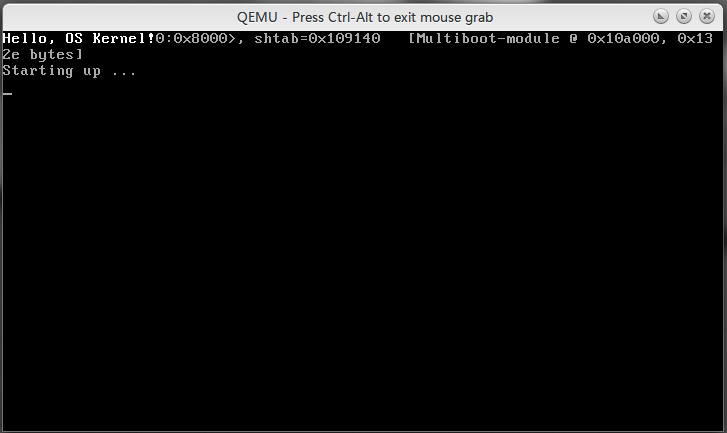
\includegraphics[scale=0.5]{picture/chapt3/hello_os_world.png}
      \caption{虚拟机里运行的 Hello, OS World!}
\end{figure}

\par 至于代码是什么意思大家先不用纠结,下一章将详细探究。

\par 辛苦了这么久,终于看到一点点成功了。有没有一点小兴奋呢?下一章我们将完全的实现对屏幕的字符输出控制,并且有机会的话我将把这个小内核运行在物理机上,和大家一起体验一下物理机运行的感觉。

\par 真正的好戏从下一章开始,别走开哦。


% 第4章
% -*- coding: UTF-8 -*-
% hurlex-chapt4.tex
% hurlex 开发文档 第4章内容

\section {字符模式下的显卡驱动}

\par 本章将开始描述内核对屏幕输出的控制。

\subsection{1MB以下的地址空间分布}

\par 在第二章我们简单的谈过地址空间的概念,并提到4G的地址空间并非全部指向主存储器,而是有部分的地址分给了其他外设。特别地,在地址空间的最低1MB处,有很多地址是属于外部设备的,下图描绘了该处地址映射的分布情况:

\begin{figure}[ht]
      \centering
      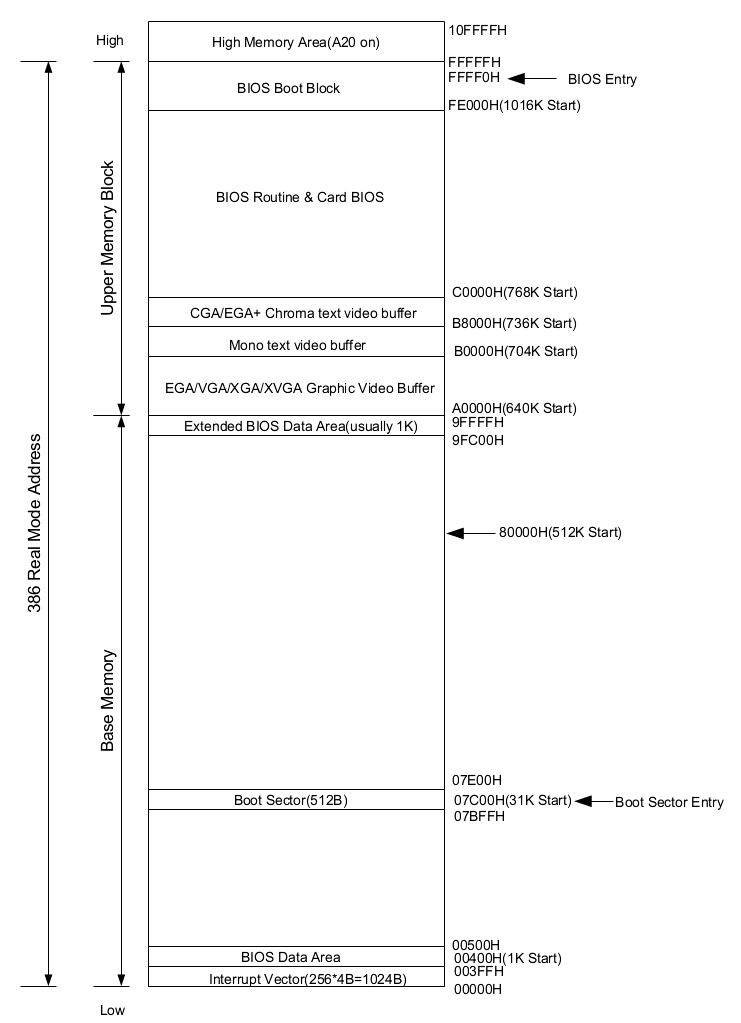
\includegraphics[scale=0.65]{picture/chapt4/BIOS-mem.png}
      \caption{低端地址空间的映射关系}
\end{figure}

\par 在PC上要显示文字,通常需要显示器和显卡这两个硬件设备。一般来说显卡负责提供显示内容,并控制具体的显示模块和状态。显示器的职责是负责将显卡呈递的内容可视化的显示出来。既然显卡需要控制显示的数据,自然就需要存储这些待显示的内容,所以显卡就有自己的存储区域。这个存储区域叫做显示存储器(Video RAM,VRAM),简称显存。当然,访问显存就需要地址。CGA/EGA+ Chroma text video buffer 这个区域映射的就是工作在文本模式的显存。同时显卡还有另外一个工作模式叫做图形模式,这个模式是目前最最常用的模式。

\subsection{显卡在文本模式下的显示规则}

\par 我们知道,对于一个字符的编码通常有输入码、内码和字模码三种。其中字模码定义了一个字符在屏幕上显示的点阵坐标。通常显卡内置一套关于基本英文字符的显示是很容易做到的,而内置汉字的显示就较为麻烦。\footnote{曾经有类似于"汉卡"之类的硬件出现,后来随着计算机处理速度的发展,这些工作一般由软件来负责了。}在这篇文档中我们只使用显卡的文本模式,不会涉及到图形模式的内容。因为一旦使用了图形模式的内容,我们就需要自行定义字符的字模码了,这很繁琐而且对我们理解操作系统原理的意义不是很大。所以我们只使用显卡的文本模式进行屏幕显示控制。所有在PC上工作的显卡,在加电初始化之后都会自动初始化到80*25的文本模式。\footnote{显卡还有其它分辨率的图形工作模式,但本文档不涉及。}在这个模式下,屏幕被划分为25行,每行可以显示80个字符,所以一屏可以显示2000个字符。上图中的0xB8000~0xBFFFF这个地址段便是映射到文本模式的显存的。当访问这些地址的时候,实际上读写的是显存区域,而显卡会周期性的读取这里的数据,并且把它们按顺序显示在屏幕上。

\par 那么,按照什么规则显示呢?这就要谈到内码了。内码定义了字符在内存中存储的形式,而英文编码就是大家所熟知的ASCII(American Standard Code for Information Interchange,美国信息交换标准代码)码了。对应的关系很简单,从0xB8000这个地址开始,每2个字节表示屏幕上显示的一个字符。从屏幕的第一行开始对应,一行接着一行的对应下去。而这两个字节的前一个是显示字符的ASCII码,后一个是控制这个字符颜色和属性的控制信息,这个字节的8个bit位表示不同的含义。每一位的含义如图所示:

\begin{figure}[ht]
      \centering
      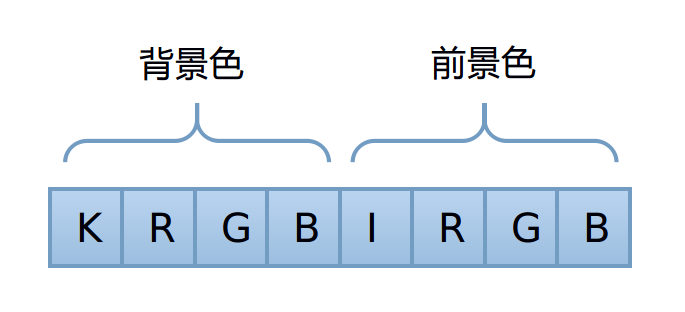
\includegraphics[scale=0.25]{picture/chapt4/char_color.png}
      \caption{字符属性示意图}
\end{figure}

\par 这些位的组合效果如下图所示:

\begin{figure}[ht]
      \centering
      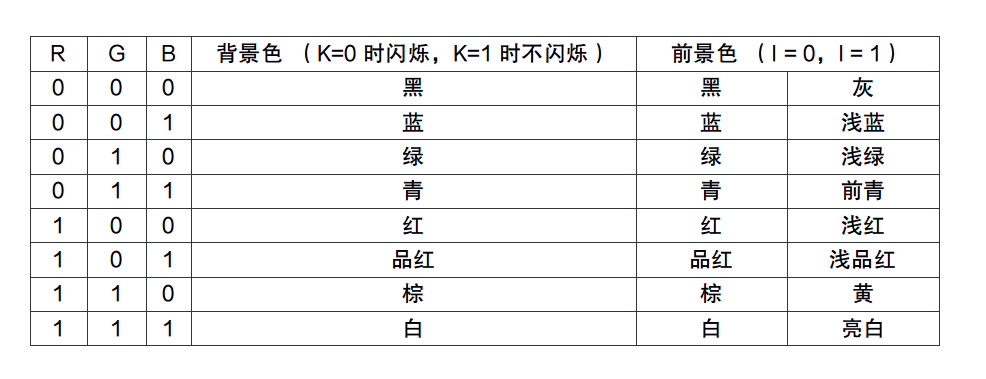
\includegraphics[scale=0.4]{picture/chapt4/text_mode_color.png}
      \caption{显卡文本模式的颜色表}
\end{figure}

\par 这两张图可以帮助我们在显卡的字符模式显示彩色的文本了,懂得这些原理对于探索性质的显示也就足够了。

\par 理解了显卡文本模式的原理之后接下来就是对屏幕显示控制编码了。不过显卡除了显示内容的存储单元之外,还有部分的显示控制单元需要了解。这些显示控制单元被编制在了独立的I/O空间里,需要用特殊的in/out指令去读写。这里相关的控制寄存器多达300多个,显然无法一一映射到I/O端口的地址空间。对此工程师们解决方案是,将一个端口作为内部寄存器的索引:0x3D4,再通过0x3D5端口来设置相应寄存器的值。

\subsection{端口读写函数的实现}

\par 在具体的设置之前,我们首先需要几个端口读写函数的实现。因为C语言并没有直接操作端口的方法,而且频繁的内联汇编麻烦又容易出错。所以好的做法就是定义几个端口读写函数。代码如下:

\begin{lstlisting}[language = C, caption = libs/common.c]
#include "common.h"

// 端口写一个字节
inline void outb(uint16_t port, uint8_t value)
{
	asm volatile ("outb %1, %0" : : "dN" (port), "a" (value));
}

// 端口读一个字节
inline uint8_t inb(uint16_t port)
{
	uint8_t ret;

	asm volatile("inb %1, %0" : "=a" (ret) : "dN" (port));

	return ret;
}

// 端口读一个字
inline uint16_t inw(uint16_t port)
{
	uint16_t ret;

	asm volatile ("inw %1, %0" : "=a" (ret) : "dN" (port));

	return ret;
}
\end{lstlisting}

\par 对应的头文件如下:
\begin{lstlisting}[language = C, caption = include/common.h]
#ifndef INCLUDE_COMMON_H_
#define INCLUDE_COMMON_H_

#include "types.h"

// 端口写一个字节
void outb(uint16_t port, uint8_t value);

// 端口读一个字节
uint8_t inb(uint16_t port);

// 端口读一个字
uint16_t inw(uint16_t port);

#endif // INCLUDE_COMMON_H_
\end{lstlisting}

\par 细心的读者想必已经发现了函数定义之前的inline关键字了吧?这是GNU对ANSI C的扩展,它和C++语言里的inline的作用是一样的。函数前面加上inline之后,编译器会尝试\footnote{没错,是尝试。内联对编译来说只是一个建议,编译器有权利根据实际情况自由处理。}在该函数的调用点直接进行代码展开,而不是传统的函数调用。这么做既有传统函数的好处,即避免了重复性的编码,减少了出错的几率。又减少了函数的调用,提高了代码的执行效率。另外,你可能见过宏函数这种用法,但是宏函数是没有参数类型的检查的,相比inline还是逊了一筹。

\subsection{颜色的枚举定义和屏幕操作函数的实现}

\par 接下来是颜色定义的枚举和一些屏幕控制函数的声明。代码如下:
\begin{lstlisting}[language = C, caption = include/console.h]
#ifndef INCLUDE_CONSOLE_H_
#define INCLUDE_CONSOLE_H_

#include "types.h"

typedef
enum real_color {
	rc_black = 0,
	rc_blue = 1,
	rc_green = 2,
	rc_cyan = 3,
	rc_red = 4,
	rc_magenta = 5,
	rc_brown = 6,
	rc_light_grey = 7,
	rc_dark_grey = 8,
	rc_light_blue = 9,
	rc_light_green = 10,
	rc_light_cyan = 11,
	rc_light_red = 12,
	rc_light_magenta = 13,
	rc_light_brown  = 14, 	// yellow
	rc_white = 15
} real_color_t;

// 清屏操作
void console_clear();

// 屏幕输出一个字符  带颜色
void console_putc_color(char c, real_color_t back, real_color_t fore);

// 屏幕打印一个以 \0 结尾的字符串  默认黑底白字
void console_write(char *cstr);

// 屏幕打印一个以 \0 结尾的字符串  带颜色
void console_write_color(char *cstr, real_color_t back, real_color_t fore);

// 屏幕输出一个十六进制的整型数
void console_write_hex(uint32_t n, real_color_t back, real_color_t fore);

// 屏幕输出一个十进制的整型数
void console_write_dec(uint32_t n, real_color_t back, real_color_t fore);

#endif  // INCLUDE_CONSOLE_H_
\end{lstlisting}

\par 参照着前面的表格,理解颜色的枚举类型并不困难。接下来是显存起始位置和当前输出的屏幕位置的变量定义。同时,我们将屏幕抽象为一个80*25的二维数组,每个数组成员都是2个字节,表示屏幕上显示的一个字符。

\begin{lstlisting}[language = C, caption = drivers/console.c]
// VGA 的显示缓冲的起点是 0xB8000
static uint16_t *video_memory = (uint16_t *)0xB8000;

// 屏幕"光标"的坐标
static uint8_t cursor_x = 0;
static uint8_t cursor_y = 0;
\end{lstlisting}

\par 请大家留意这里变量定义时候的 static 限定符,当一个全局变量或者函数只在本模块文件内被使用时,最好限定其作用域。每个模块应当尽可能的向外部暴露较少的接口。

\subsubsection{屏幕输入光标的移动}

\par 在本模块内,cursor\_x 和 cursor\_y 这两个变量指明了逻辑上的当前输出位置,但是并没有实际上移动硬件的显示"光标",下面的函数实现了根据这两个变量的值移动光标的功能。

\begin{lstlisting}[language = C, caption = drivers/console.c]
static void move_cursor()
{
	// 屏幕是 80 字节宽
	uint16_t cursorLocation = cursor_y * 80 + cursor_x;
	
	// 在这里用到的两个内部寄存器的编号为14与15,分别表示光标位置
	// 的高8位与低8位。

	outb(0x3D4, 14); 			// 告诉 VGA 我们要设置光标的高字节
	outb(0x3D5, cursorLocation >> 8); 	// 发送高 8 位
	outb(0x3D4, 15); 			// 告诉 VGA 我们要设置光标的低字节
	outb(0x3D5, cursorLocation);      	// 发送低 8 位
}
\end{lstlisting}

\par 这里的端口和设置值都是固定的,也没有什么道理可讲。虽然显卡的各项技术发展的很快,但是这个原始的VGA标准被所有显卡完整的保存了下来。

\subsubsection{清屏操作}

\par 然后是清屏操作,其实这里的"清屏"很简单,其实就是用白底黑字的"空格符"覆盖整个屏幕的显示区域罢了。这么做自然就实现了我们想要的"清屏"操作了。代码很简单:

\begin{lstlisting}[language = C, caption = drivers/console.c]
void console_clear()
{
	uint8_t attribute_byte = (0 << 4) | (15 & 0x0F);
	uint16_t blank = 0x20 | (attribute_byte << 8);

	int i;
	for (i = 0; i < 80 * 25; i++) {
	      video_memory[i] = blank;
	}

	cursor_x = 0;
	cursor_y = 0;
	move_cursor();
}
\end{lstlisting}

\subsubsection{屏幕滚动显示}

\par 那么屏幕滚动呢?用C语言来描述实际上就是将后24行的数据全部向上挪动一行,最后一行清空罢了,就是这么简单。

\begin{lstlisting}[language = C, caption = drivers/console.c]
static void scroll()
{
	// attribute_byte 被构造出一个黑底白字的描述格式
	uint8_t attribute_byte = (0 << 4) | (15 & 0x0F);
	uint16_t blank = 0x20 | (attribute_byte << 8);  // space 是 0x20

	// cursor_y 到 25 的时候,就该换行了
	if (cursor_y >= 25) {
		// 将所有行的显示数据复制到上一行,第一行永远消失了...
		int i;
		
		for (i = 0 * 80; i < 24 * 80; i++) {
		      video_memory[i] = video_memory[i+80];
		}

		// 最后的一行数据现在填充空格,不显示任何字符
		for (i = 24 * 80; i < 25 * 80; i++) {
		      video_memory[i] = blank;
		}
		
		// 向上移动了一行,所以 cursor_y 现在是 24
		cursor_y = 24;
	}
}
\end{lstlisting}

\subsubsection{显示字符串}

\par 那么屏幕显示字符串呢?我们可以先实现"屏幕显示一个字符"的函数,那么"屏幕显示一个字符串"不就可以了么?这几个函数的实现如下:

\begin{lstlisting}[language = C, caption = drivers/console.c]
void console_putc_color(char c, real_color_t back, real_color_t fore)
{
	uint8_t back_color = (uint8_t)back;
	uint8_t fore_color = (uint8_t)fore;

	uint8_t attribute_byte = (back_color << 4) | (fore_color & 0x0F);
	uint16_t attribute = attribute_byte << 8;

	// 0x08 是退格键的 ASCII 码
	// 0x09 是tab 键的 ASCII 码
	if (c == 0x08 && cursor_x) {
	      cursor_x--;
	} else if (c == 0x09) {
	      cursor_x = (cursor_x+8) & ~(8-1);
	} else if (c == '\r') {
	      cursor_x = 0;
	} else if (c == '\n') {
		cursor_x = 0;
		cursor_y++;
	} else if (c >= ' ') {
		video_memory[cursor_y*80 + cursor_x] = c | attribute;
		cursor_x++;
	}

	// 每 80 个字符一行,满80就必须换行了
	if (cursor_x >= 80) {
		cursor_x = 0;
		cursor_y ++;
	}

	// 如果需要的话滚动屏幕显示
	scroll();

	// 移动硬件的输入光标
	move_cursor();
}

void console_write(char *cstr)
{
	while (*cstr) {
	      console_putc_color(*cstr++, rc_black, rc_white);
	}
}

void console_write_color(char *cstr, real_color_t back, real_color_t fore)
{
	while (*cstr) {
	      console_putc_color(*cstr++, back, fore);
	}
}
\end{lstlisting}

\par 代码里唯一需要注意的便是输出后要检查当前的位置和判断一些特殊的符号表示的操作,例如换行之类的实现。同时一定要注意修改存储当前位置的两个变量和移动屏幕上的光标,而且屏幕输出满了以后要上滚。我们暂时不考虑诸如屏幕翻页之类的功能。至于屏幕输出十六进制数字和十进制数字的函数请大家自己实现,相信这并不困难。

\subsection{测试屏幕操作函数}

\par 屏幕的操作到这里就告一段落了,我们修改下初始化函数,感受一下今天的成果吧。

\begin{lstlisting}[language = C, caption = init/entry.c]
#include "console.h"

int kern_entry(multiboot_t *mboot_ptr)
{
	console_clear();

	console_write_color("Hello, OS kernel!\n", rc_black, rc_green);

	return 0;
}
\end{lstlisting}

\par 编译运行,干净的屏幕上出现了我们绿色的文字,还有下一行闪烁着的输入光标。

\begin{figure}[ht]
      \centering
      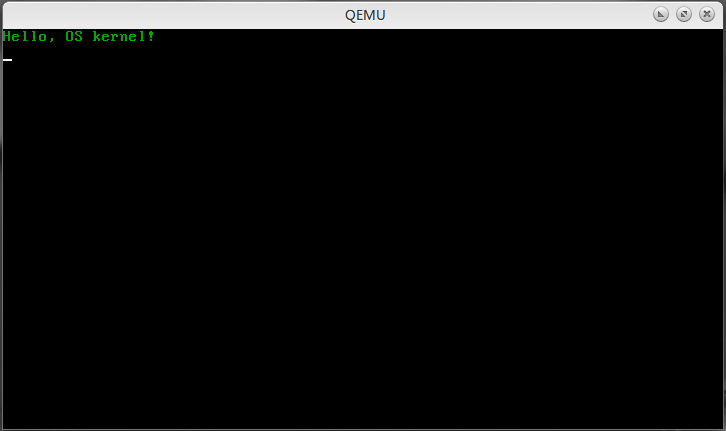
\includegraphics[scale=0.6]{picture/chapt4/hello_os_world_green.png}
      \caption{屏幕输出控制的展示}
\end{figure}

\par 本章的内容到这里就结束了,下一章我们缓缓脚步,来完成一些更重要的模块。


% 第5章
% -*- coding: UTF-8 -*-
% hurlex-chapt5.tex
% hurlex 开发文档 第5章内容

\section {相关库函数和调试打印函数}

\par 截至前四章,我们已经实现了一个能在屏幕上任意输出字符的小内核了。但是在开始新的探索之前,需要完成一些在内核开发中至关重要的模块。

\subsection {C语言的字符串处理函数}

\par 我们之前多次提到现有的用户态的C语言标准库无法在内核中使用,但是内核开发中难免要用到诸如字符串操作的函数,所以我们需要自己实现这些字符串相关的函数。

\par 首先给出函数的声明:

\begin{lstlisting}[language = C, caption = include/string.h]
#ifndef INCLUDE_STRING_H_
#define INCLUDE_STRING_H_

#include "types.h"

void memcpy(uint8_t *dest, const uint8_t *src, uint32_t len);

void memset(void *dest, uint8_t val, uint32_t len);

void bzero(void *dest, uint32_t len);

int strcmp(const char *str1, const char *str2);

char *strcpy(char *dest, const char *src);

char *strcat(char *dest, const char *src);

int strlen(const char *src);

#endif 	// INCLUDE_STRING_H_
\end{lstlisting}

\par 至于函数的实现我只给出其中几个函数的参考实现,剩下的请大家自己实现吧,考验大家C语言指针基本功的时候到了。\footnote{友情提醒,这里的函数最好在用户态下进行编码和测试,确认正确无误了再放入内核中使用。}

\begin{lstlisting}[language = C, caption = libs/string.c]
#include "string.h"

inline void memcpy(uint8_t *dest, const uint8_t *src, uint32_t len)
{
	for (; len != 0; len--) {
		*dest++ = *src++;
	}
}

inline void memset(void *dest, uint8_t val, uint32_t len)
{
	uint8_t *dst = (uint8_t *)dest;

	for ( ; len != 0; len--) {
		*dst++ = val;
	}
}

inline void bzero(void *dest, uint32_t len)
{
	memset(dest, 0, len);
}
\end{lstlisting}

\subsection {内核级的屏幕打印函数}

\par 初学C语言时使用的printf函数想必大家都很熟悉吧?可是在这里是没有办法使用现有的库的。不过完成了屏幕的控制输出之后,我们就可以基于它同时根据printf函数的实现原理,写出一个内核态下可以进行屏幕打印的函数printk了。但是这里恐怕不敢展开来讲,这涉及到C语言的可变形参表\footnote{也有译作"变长参数"或"可变参数列表"的。}和函数调用栈等繁多细节。原本我只想给出具体的实现以供大家参考,但是又觉得带给大家"夹生饭"的做法不太好。所以我简单的结合代码给大家阐述下基本的实现原理,同时希望没理解的读者自行检索相关资料,争取理解这个函数的实现。

\par 我们之前已经实现过了屏幕打印字符串和数字等内容的函数了,那么此时想实现printf函数,难点就在于构造这个最终打印的字符串。现在摆在我们面前的问题其实只有两个,那就是如何知道有多少个参数传进来和如何知道每一个参数的类型。其实我们完全可以照搬printf的做法,提供同样的接口。printf的用法大家很清楚,首先是一个待显示的字符串,里面分别用\%加相关字母的方式一一指明了后面的参数数量和类型。只要我们传递正确的带有格式描述的字符串和相关参数,printf函数就能正确的打印出来结果。

\par 我们的printk函数的实现完全模仿printf函数的接口,首先是函数声明:\footnote{这里的debug.h是一部分,后面给出完整的debug.h的代码。}

\begin{lstlisting}[language = C, caption = include/debug.h]
#include "console.h"
#include "vargs.h"

// 内核的打印函数
void printk(const char *format, ...);

// 内核的打印函数 带颜色
void printk_color(real_color_t back, real_color_t fore, const char *format, ...);
\end{lstlisting}

\par 后面一个printk\_color对应之前的带颜色的屏幕输出,因为C语言没有C++那样的函数重载或者默认参数的特性,所以我们只能定义两个函数了。printk函数的声明的参数列表首先是一个字符串,然后是三个小数点,这样的话编译器会允许我们在调用printk函数的时候带有任意多个实参了。剩下的问题就是在printk的实现里,如何在没有形参名的情况下找到取到每一个参数。解决了这个问题之后,剩下的问题就很简单了。

\par 我们先贴出另一个所需要的头文件 vargs.h 的内容:

\begin{lstlisting}[language = C, caption = include/vargs.h]
#ifndef INCLUDE_VARGS_H_
#define INCLUDE_VARGS_H_

typedef __builtin_va_list va_list;

#define va_start(ap, last)         (__builtin_va_start(ap, last))
#define va_arg(ap, type)           (__builtin_va_arg(ap, type))
#define va_end(ap) 

#endif 	// INCLUDE_VARGS_H_
\end{lstlisting}

\par 我们定义了几个宏,这几个宏用于取得每一个调用printk函数时传入的参数值。可能你会很诧异va\_list、\_\_builtin\_va\_start和\_\_builtin\_va\_arg这几个类似于函数东西在何处定义,其实它们是gcc内置的变量和函数之类的存在了。GNU C提供了很多扩展,这只是其中的一个。而其他平台上通常把它们定义为宏,下面是一个简化版的定义:\footnote{注意这里是简化版的定义,事实上出于x86压栈元素长度的限制和优化的考虑,小于等于4字节的类型统一扩展到4字节压栈。大于4字节小于等于8字节的类型统一以8字节压栈(另外32位压栈指令的操作数只能是16位或者32位的)。}

\begin{lstlisting}[language = C, caption = 可变形参表]
#define  va_list              char *

#define  va_start(p, first)   (p = (va_list)&first + sizeof(first))
#define  va_arg(p, next)      (*(next*)((p += sizeof(next) ) - sizeof(next)))
#define  va_end(p)            (p = (va_list)NULL)
\end{lstlisting}

\par 我们可以看到,这几个宏的作用是根据第一个参数的地址和类型,通过逐渐计算出以后每一个参数的起始地址的方法取出每一个参数。也就是说,这是建立在"函数调用的参数在内存里是连续的"这一简单假设之上的。

\par 我们知道函数调用是通过栈来传递参数的,那参数按照什么顺序入栈?入栈后使用完参数后何处的代码清理之前栈里的参数呢?事实上传递参数的工作必须由函数调用者和函数本身来协调,即就是所谓的"调用约定"。现行的调用约定有很多中,而C语言默认的调用约定就是cdecl了,cdecl约定规定由调用者从右向左向栈里连续的压入参数,在函数返回之后,再清理掉压入的参数以保证堆栈平衡。对于类似于 func(1, 2, 3, 4); 这样的函数调用编译后生成的汇编代码类似下面这样:

\begin{lstlisting}[language = {[x86masm]Assembler}, caption = 函数调用]
	push 4
	push 3
	push 2
	push 1
	call func
	sub esp, 16
\end{lstlisting}

\par 大家看明白没有?默认情况下按照cdecl约定,参数被从右向左连续压栈了,而且调用完后根据参数长度自行清理了参数。\footnote{当然C语言中调用处理这一步是编译器自动生成的,明白了原理之后我们只要实现具体的函数即可。}明白了这些,我们就为以后的汇编和C语言函数的相互调用打好了基础。而且也明白了参数在栈里面是连续的存储的,只要知道了第一个参数在栈里的地址和每个参数的类型,就能计算出每一个参数的地址访问到它们了。

\par printk涉及的代码比较多,没有办法在这里一一细说了。还是那句话,需要大家主动的去探索学习。这个项目使用的printk甚至直接参考和复制了Linux早期内核里的一些思想和子函数的实现,希望大家自己去研究一下。至于使用的方法就很简单了,它和大家熟悉的printf函数没有什么太大差异。

\subsection{代码级调试的实现}

\par 不知道大家之前的编码过程是否顺利?是否遇到了运行后无法得出结果的问题?我们平时构建用户级程序的时候,有很长一段时间和精力都是在调试。那这个小内核能否像平时那样轻松的调试查错?如果不能或者只能进行汇编级别的调试,恐怕会对我们的后期开发造成很大的影响。毕竟在客观上bug一就避免不了,那我们能否使用平日里习惯的调试工具进行轻松的排错?答案是肯定的。我们给出的解决方案就是使用qemu联合gdb进行C语言源代码级别的调试。具体怎么做呢?

\par 首先是通讯问题,因为qemu和gdb运行的时候毕竟是两个进程,数据交换必然涉及到进程间通信机制。所幸它们都支持一个标准的调试协议,而且开启的方法都很简单。qemu使用以下命令启动即可:

\begin{Verbatim}[frame=single]
  qemu -S -s -fda floppy.img -boot a 
\end{Verbatim}

\par 这几个参数中 -fda floppy.img 和 -boot a 是指定启动的镜像,-s 这个参数指的是启动时开启1234端口等待gdb连接(这个参数从字面上看比较隐晦),-S 是指启动时不自动开始运行,等待调试器的执行命令。以调试模式启动了虚拟机之后,再启动gdb。需要注意的是,此时的gdb没有内核程序的符号文件,没有办法进行代码级调试。解决的办法很简单,我们使用命令加载待调试内核对应的可执行文件即可。\footnote{别忘了我们的Makefile中的编译参数中指明了生成内核的调试信息。}启动了gdb之后,我们依次执行以下指令即可。

\begin{Verbatim}[frame=single]
  file hx_kernel
  target remote :1234
  break kern_entry
  c
\end{Verbatim}

\par 这几个命令的意思分别是加载待调试文件的符号信息;连接本地的1234端口;在 kern\_entry 函数处下断点;执行到断点处。\footnote{之前修改过Makefile中生成的内核文件名的读者们注意这里必须和实际的内核文件名保持一致。}如果每次调试都需要这样做的话也未免太麻烦了,所以我们可以把上面几条命令写在scripts目录里的gdbinit文件里,在启动gdb的时候自动加载执行。甚至在Makefile里也有我写的一个专门用于调试的伪目标debug 。在开始测试前,先给出我此时的目录结构以便大家核对。

\begin{Verbatim}[frame=single]
.
|-- boot
|   `-- boot.s
|-- drivers
|   `-- console.c
|-- floppy.img
|-- include
|   |-- common.h
|   |-- console.h
|   |-- debug.h
|   |-- string.h
|   |-- types.h
|   `-- vargs.h
|-- init
|   `-- entry.c
|-- kernel
|   `-- debug
|       |-- debug.c
|       `-- printk.c
|-- libs
|   |-- common.c
|   `-- string.c
|-- Makefile
`-- scripts
    |-- gdbinit
    `-- kernel.ld
    
    8 directories, 17 files
\end{Verbatim}

\par 现在开始调试测试,执行以下命令开始调试。\footnote{我使用的是cgdb,这是一个给gdb提供了代码高亮显示的前端,你可以安装它或者修改Makefile里面debug项目下的 cgdb -x scripts/gdbinit 为 gdb -tui -x scripts/gdbinit}

\begin{Verbatim}[frame=single]
  make
  make debug
\end{Verbatim}

\par 源码级的调试效果如图:

\begin{figure}[ht]
      \centering
      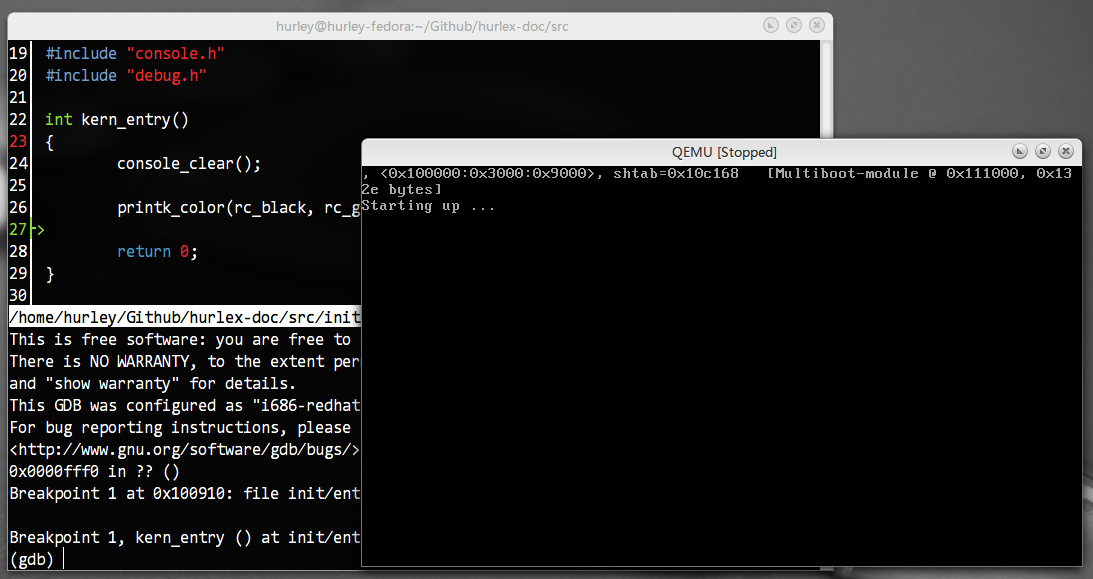
\includegraphics[scale=0.4]{picture/chapt5/os_debug.png}
      \caption{源码级别调试内核}
\end{figure}

\par 剩下的调试操作和平时使用gdb的方法别无二致,所以大家应该都不陌生。有的读者可能需要学习一些查看寄存器值之类的命令,请查阅手册吧。

\subsection{打印函数调用栈}

\par 解决了代码级调试的功能,我们来完成一些稍微复杂的函数,那就是当内核遇到致命错误时,如何自动打印当前的函数调用栈?这涉及到GRUB Multiboot规范的很多细节和函数调用栈的结构。我们先从Multiboot的细节说起。

\par 在boot/boot.s里的start函数调用kern\_entry函数之前,我们把ebx寄存器的值赋给了一个全局变量glb\_mboot\_ptr。这是一个指向了multiboot\_t类型结构体的指针,这个结构体存储了GRUB在调用内核前获取的硬件信息和内核文件本身的一些信息。我们先给出具体的结构体的定义:

\begin{lstlisting}[language = C, caption = include/multiboot.h]
#ifndef INCLUDE_MULTIBOOT_H_
#define INCLUDE_MULTIBOOT_H_

#include "types.h"

typedef
struct multiboot_t {
	uint32_t flags;		// Multiboot 的版本信息
	/** 
	 * 从 BIOS 获知的可用内存
	 *
	 * mem_lower 和 mem_upper 分别指出了低端和高端内存的大小,单位是K。
	 * 低端内存的首地址是 0 ,高端内存的首地址是 1M 。
	 * 低端内存的最大可能值是 640K 
	 * 高端内存的最大可能值是最大值减去 1M 。但并不保证是这个值。
	 */
	uint32_t mem_lower;
	uint32_t mem_upper;

	uint32_t boot_device;	// 指出引导程序从哪个BIOS磁盘设备载入的OS映像
	uint32_t cmdline;	// 内核命令行
	uint32_t mods_count;	// boot 模块列表
	uint32_t mods_addr;
	
	/**
	 * ELF 格式内核映像的 section 头表。包括每项的大小、一共有几项以及作为名字索引
	 * 的字符串。
	 */
	uint32_t num;
	uint32_t size;
	uint32_t addr;
	uint32_t shndx;

	/**
	 * 以下两项指出保存由 BIOS 提供的内存分布的缓冲区的地址和长度
	 * mmap_addr 是缓冲区的地址, mmap_length 是缓冲区的总大小
	 * 缓冲区由一个或者多个下面的 mmap_entry_t 组成
	 */
	uint32_t mmap_length;		
	uint32_t mmap_addr;
	
	uint32_t drives_length; 	// 指出第一个驱动器结构的物理地址	
	uint32_t drives_addr; 		// 指出第一个驱动器这个结构的大小
	uint32_t config_table; 		// ROM 配置表
	uint32_t boot_loader_name; 	// boot loader 的名字
	uint32_t apm_table; 	    	// APM 表
	uint32_t vbe_control_info;
	uint32_t vbe_mode_info;
	uint32_t vbe_mode;
	uint32_t vbe_interface_seg;
	uint32_t vbe_interface_off;
	uint32_t vbe_interface_len;
} __attribute__((packed)) multiboot_t;

/**
 * size 是相关结构的大小,单位是字节,它可能大于最小值 20
 * base_addr_low 是启动地址的低32位,base_addr_high 是高 32 位,启动地址总共有 64 位
 * length_low 是内存区域大小的低32位,length_high 是内存区域大小的高 32 位,总共是 64 位
 * type 是相应地址区间的类型,1 代表可用 RAM,所有其它的值代表保留区域
 */
typedef
struct mmap_entry_t {
	uint32_t size; 		// size 是不含 size 自身变量的大小
	uint32_t base_addr_low;
	uint32_t base_addr_high;
	uint32_t length_low;
	uint32_t length_high;
	uint32_t type;
} __attribute__((packed)) mmap_entry_t;

// 声明全局的 multiboot_t * 指针
extern multiboot_t *glb_mboot_ptr;

#endif 	// INCLUDE_MULTIBOOT_H_
\end{lstlisting}

\par 结构体中有很多注释,大家结合具体的协议文档很容易就可以看懂。我们暂时需要关心的主要是符号表,其它的信息我们在之后用到的时候再讨论。也就是说,我们暂时只关注结构体中以下几个字段的内容即可:

\begin{lstlisting}[language = C, caption = include/multiboot.h]
	......
	/**
	 * ELF 格式内核映像的 section 头表。
	 * 包括每项的大小、一共有几项以及作为名字索引的字符串表。
	 */
	uint32_t num;
	uint32_t size;
	uint32_t addr;
	uint32_t shndx;
	......
\end{lstlisting}

要理解下面的内容还真有些困难,因为它涉及的面太广了。我们先以ELF的文件格式做为切入点。我们先添加elf.h这个头文件:

\begin{lstlisting}[language = C, caption = include/elf.h]
#ifndef INCLUDE_ELF_H_
#define INCLUDE_ELF_H_

#include "types.h"
#include "multiboot.h"

#define ELF32_ST_TYPE(i) ((i)&0xf)

// ELF 格式区段头
typedef
struct elf_section_header_t {
  uint32_t name;
  uint32_t type;
  uint32_t flags;
  uint32_t addr;
  uint32_t offset;
  uint32_t size;
  uint32_t link;
  uint32_t info;
  uint32_t addralign;
  uint32_t entsize;
} __attribute__((packed)) elf_section_header_t;

// ELF 格式符号
typedef
struct elf_symbol_t {
  uint32_t name;
  uint32_t value;
  uint32_t size;
  uint8_t  info;
  uint8_t  other;
  uint16_t shndx;
} __attribute__((packed)) elf_symbol_t;

// ELF 信息
typedef
struct elf_t {
  elf_symbol_t *symtab;
  uint32_t      symtabsz;
  const char   *strtab;
  uint32_t      strtabsz;
} elf_t;

// 从 multiboot_t 结构获取ELF信息
elf_t elf_from_multiboot(multiboot_t *mb);

// 查看ELF的符号信息
const char *elf_lookup_symbol(uint32_t addr, elf_t *elf);

#endif 	// INCLUDE_ELF_H_
\end{lstlisting}

\par 这段结构体定义里包含了ELF文件的区段头、符号表等信息。我们给出从multiboot\_t结构中提取出ELF相关信息的代码:

\begin{lstlisting}[language = C, caption = kernel/debug/elf.c]
#include "common.h"
#include "string.h"
#include "elf.h"

// 从 multiboot_t 结构获取ELF信息
elf_t elf_from_multiboot(multiboot_t *mb)
{
	int i;
	elf_t elf;
	elf_section_header_t *sh = (elf_section_header_t *)mb->addr;

	uint32_t shstrtab = sh[mb->shndx].addr;
	for (i = 0; i < mb->num; i++) {
		const char *name = (const char *)(shstrtab + sh[i].name);
		// 在 GRUB 提供的 multiboot 信息中寻找
		// 内核 ELF 格式所提取的字符串表和符号表
		if (strcmp(name, ".strtab") == 0) {
			elf.strtab = (const char *)sh[i].addr;
			elf.strtabsz = sh[i].size;
		}
		if (strcmp(name, ".symtab") == 0) {
			elf.symtab = (elf_symbol_t*)sh[i].addr;
			elf.symtabsz = sh[i].size;
		}
	}

	return elf;
}

// 查看ELF的符号信息
const char *elf_lookup_symbol(uint32_t addr, elf_t *elf)
{
	int i;

	for (i = 0; i < (elf->symtabsz / sizeof(elf_symbol_t)); i++) {
		if (ELF32_ST_TYPE(elf->symtab[i].info) != 0x2) {
		      continue;
		}
		// 通过函数调用地址查到函数的名字
		if ( (addr >= elf->symtab[i].value) && (addr < (elf->symtab[i].value + elf->symtab[i].size)) ) {
			return (const char *)((uint32_t)elf->strtab + elf->symtab[i].name);
		}
	}

	return NULL;
}
\end{lstlisting}

\par 我们之前多次提过GRUB在载入内核之后,会读取ELF并把相关的信息组织成结构体放在multiboot\_t结构,并把结构体指针放在ebx寄存器里传递给内核。其multiboot\_t结构的addr成员便指向的是elf\_section\_header\_t类型的结构体数组,num成员是这个结构体数组的成员个数。

\par 这里的代码可能让大家一下子有点蒙,如果你觉得无从下手的话不妨在纸上画一画这几个结构体的关系图,这能帮助你理解。对于这里的代码大家不必过于深究,毕竟ELF格式只是Linux平台下的一种可执行格式,而本文档的目的只是想让大家建立对项目的整体把握,细节问题就留给大家自己去理解吧。\footnote{objdump和readelf等工具是探索ELF格式的利器,它们同属GNU binutils工具包的一部分。}

\par 通过以上的努力,我们获取了ELF文件中关于每个函数的名称和它们代码的区域,那么此时如何使用这些信息寻找函数名称呢?其实大家从elf\_lookup\_symbol函数的实现里就能看出来。我们提供了一个地址,然后查询这个地址在哪个函数的代码区间里,然后返回了这个函数名的字符串指针。

\par 终于到了最后的函数调用栈问题了,这也是最终的打印调用栈函数panic的实现原理。

\par 我们利用objdump文件反汇编生成的hx\_kernel文件,找到入口函数的代码结合start函数的实现一起分析。反汇编的指令如下:

\begin{Verbatim}[frame=single]
  objdump -M intel -d hx_kernel
\end{Verbatim}

\par -M intel 参数是生成Intel风格的汇编,想必大家对Intel风格的汇编更熟悉吧。这个命令会反汇编所有的函数,我们找到start函数和kern\_entry函数的反汇编代码如下:

\begin{lstlisting}[language = {[x86masm]Assembler}, caption = 入口函数反汇编]
0010000c <start>:
  10000c:	fa                   	cli    
  10000d:	89 1d 00 b0 10 00    	mov    DWORD PTR ds:0x10b000,ebx
  100013:	bc 03 80 00 00       	mov    esp,0x8003
  100018:	83 e4 f0             	and    esp,0xfffffff0
  10001b:	bd 00 00 00 00       	mov    ebp,0x0
  100020:	e8 af 0a 00 00       	call   100ad4 <kern_entry>
00100025 <stop>:
  100025:	f4                   	hlt    
  100026:	eb fd                	jmp    100025 <stop>

00100ad4 <kern_entry>:
  100ad4:	55                   	push   ebp
  100ad5:	89 e5                	mov    ebp,esp
  100ad7:	83 ec 18             	sub    esp,0x16
  100ada:	e8 39 01 00 00       	call   100c18 <console_clear>
  100adf:	c7 44 24 08 9b 21 10 	mov    DWORD PTR [esp+0x8],0x10219b
  100ae6:	00 
  100ae7:	c7 44 24 04 02 00 00 	mov    DWORD PTR [esp+0x4],0x2
  100aee:	00 
  100aef:	c7 04 24 00 00 00 00 	mov    DWORD PTR [esp],0x0
  100af6:	e8 33 f7 ff ff       	call   10022e <printk_color>
  100afb:	b8 00 00 00 00       	mov    eax,0x0
  100b00:	c9                   	leave  
  100b01:	c3                   	ret    
\end{lstlisting}

\par 我们从start函数开始分析。首先第2行是关闭中断,因为此时尚未设置中断相关的一些数据结构,如果发生了中断的话就会崩溃。接下来第3行是我们把ebx寄存器中存储的multiboot\_t结构的指针传给了全局变量glb\_mboot\_ptr,接着4、5行分别是初始化内核栈的栈顶指针,第5行与运算的目的是使得栈地址按照16字节对齐,这样的效率比较好。随后start函数调用了内核入口kern\_entry函数。大家注意这里的call指令实际上做了两件事情,第一件事情是将call指令之后的地址压入栈,然后跳转到kern\_entry函数的起始地址那里去。也就是说这里的call 100ad4 <kern\_entry>等价于以下两条指令:

\begin{Verbatim}[frame=single]
  push 100022
  jmp 100ad4
\end{Verbatim}

\par 我们这里碰巧有个stop的标号在这里,所以nasm处理成stop函数了。其实所有的函数在代码段里都是连续的,无论跳转到哪里,都会从该处开始执行的。现在大家思考这样一个问题,为什么要保存call指令的下一条指令的地址到栈里呢?其实很简单,因为子函数调用完会返回,不保存返回的地址的话怎么知道该往哪里返回呢。

\par 我们继续往下看,kern\_entry函数一开始就把ebp寄存器压栈,然后将esp赋给ebp寄存器。为什么要先压栈呢?因为在一个CPU核里所有的寄存器都只有一份,当执行流程从一个函数跳转到另外一个函数的时候,之前的寄存器可能保存着重要的信息。如果我们不保护之前的执行现场,当子函数执行完返回的时候就会出问题。这么多寄存器全都要保存吗?当然不是,x86的规则是这样的:寄存器分为调用者保存寄存器和被调用者保存寄存器。按照惯例,eax,edx,ecx寄存器是调用者保存,ebx,esi,edi,ebp等寄存器是被调用者负责保存。举个例子,一个函数想使用ebx寄存器那么必须在返回前恢复ebx原先的值,而使用edx寄存器就无需暂存和恢复。如果我们只用C语言编程的话自然无需关注这些,因为编译器会替我们打点这一切。但是如果要实现汇编和C语言的混合编程的话,就要留心这些了。

\par 我们回到正题。第16行的汇编指令实际上是开辟函数局部变量的操作,不过这个函数没有用到。接着又是一个函数调用,同理,压入当前指令之后一条指令的地址,然后跳转过去执行,而且之后所有的函数调用基本上都是按照这个套路进行的。当函数执行完之后,函数清理开辟的局部变量的空间,恢复在栈里保存的ebp寄存器,弹出返回地址跳转回去。这就是函数执行和返回的一个大致的流程。所以当一个函数遇到了错误的时候,我们就可以调用一个打印当前栈里的函数调用链的函数来帮助我们调试。原理很简单,所有函数的返回地址都保存在栈里,我们结合之前获取到的所有函数的名称和它们的地址区间,只要查找到这个返回地址在哪一个函数的地址区间里,就能知道之前调用的函数了。而这个查找函数我们已经实现了。

\par 不知道我刚刚的描述大家理解了没有?如果还有点迷糊的话来看下面的这张图片,这是按照上文的描述给出的函数调用栈的示意图。不过需要注意的是,所有的地址是根据我自己机器上生成的汇编地址绘制的。大家可能会有不一样的地址,但是原理是一致的。

\begin{figure}[ht]
      \centering
      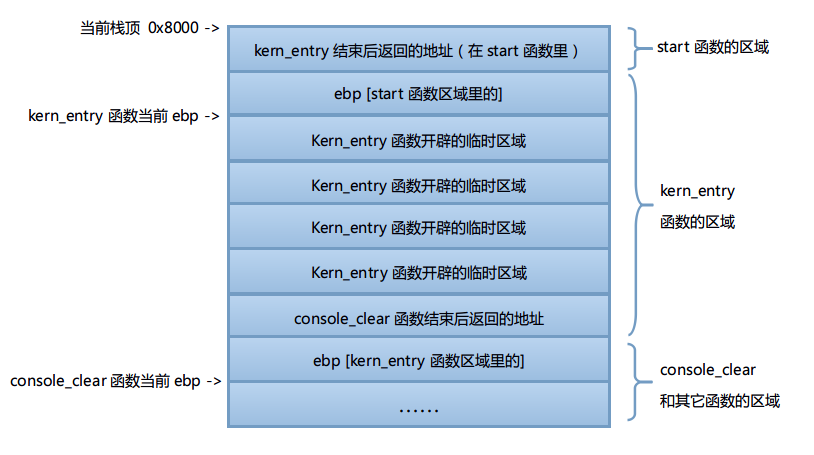
\includegraphics[scale=0.5]{picture/chapt5/os_function_stack.png}
      \caption{内核函数调用栈}
\end{figure}

\par 在示意图中我们假设从start函数->kern\_entry函数->console\_clear函数的调用过程,最终暂停在console\_clear函数里面。我们可以清楚的看到,只要拿到此时的ebp寄存器的值,就可以沿着这个调用链找到每一个调用的函数的返回地址,之前的问题就这样解决了。需要注意的是C语言里对指针做算数运算时,改变的地址长度是和当前指针变量的类型相关的。

\par 我们分别给出最终的打印函数调用信息的panic函数的声明和实现。顺带还有几个调试使用的宏,都很简单:

\begin{lstlisting}[language = C, caption = debug/debug.h]
#ifndef INCLUDE_DEBUG_H_
#define INCLUDE_DEBUG_H_

#include "console.h"
#include "vargs.h"
#include "elf.h"

#define assert(x, info)                                       	\
	do {                                                	\
		if (!(x)) {                                     \
			panic(info);     			\
		}                                               \
	} while (0)
	
// 编译期间静态检测
#define static_assert(x)                                	\
	switch (x) { case 0: case (x): ; }

// 初始化 Debug 信息
void init_debug();

// 打印当前的函数调用栈信息
void panic(const char *msg);

// 打印当前的段存器值
void print_cur_status();

// 内核的打印函数
void printk(const char *format, ...);

// 内核的打印函数 带颜色
void printk_color(real_color_t back, real_color_t fore, const char *format, ...);

#endif 	// INCLUDE_DEBUG_H_
\end{lstlisting}

\par 这里已经是debug.h头文件的完整的内容了,具体的几个实现函数一并在下面列出。

\begin{lstlisting}[language = C, caption = kernel/debug/debug.c]
#include "debug.h"

static void print_stack_trace();
static elf_t kernel_elf;

void init_debug()
{
	// 从 GRUB 提供的信息中获取到内核符号表和代码地址信息
	kernel_elf = elf_from_multiboot(glb_mboot_ptr);
}

void print_cur_status()
{
	static int round = 0;
	uint16_t reg1, reg2, reg3, reg4;

	asm volatile ( 	"mov %%cs, %0;"
			"mov %%ds, %1;"
			"mov %%es, %2;"
			"mov %%ss, %3;"
			: "=m"(reg1), "=m"(reg2), "=m"(reg3), "=m"(reg4));

	// 打印当前的运行级别
	printk("%d: @ring %d\n", round, reg1 & 0x3);
	printk("%d:  cs = %x\n", round, reg1);
	printk("%d:  ds = %x\n", round, reg2);
	printk("%d:  es = %x\n", round, reg3);
	printk("%d:  ss = %x\n", round, reg4);
	++round;
}

void panic(const char *msg)
{
	printk("*** System panic: %s\n", msg);
	print_stack_trace();
	printk("***\n");
	
	// 致命错误发生后打印栈信息后停止在这里
	while(1);
}

void print_stack_trace()
{
	uint32_t *ebp, *eip;

	asm volatile ("mov %%ebp, %0" : "=r" (ebp));
	while (ebp) {
		eip = ebp + 1;
		printk("   [0x%x] %s\n", *eip, elf_lookup_symbol(*eip, &kernel_elf));
		ebp = (uint32_t*)*ebp;
	}
}
\end{lstlisting}

\par 至此,本章要阐述的内容到此结束。我们整合所有代码,如下修改entry函数并编译运行测试一下这个打印函数调用栈的函数。

\begin{lstlisting}[language = C, caption = init/entry.c]
#include "console.h"
#include "debug.h"

int kern_entry()
{
	init_debug();

	console_clear();

	printk_color(rc_black, rc_green, "Hello, OS kernel!\n");

	panic("test");

	return 0;
}
\end{lstlisting}

\par 运行结果如图:

\begin{figure}[ht]
      \centering
      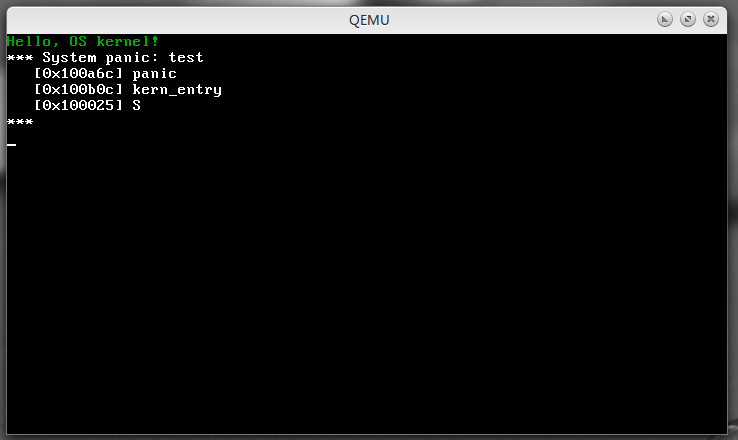
\includegraphics[scale=0.5]{picture/chapt5/os_panic.png}
      \caption{panic 函数测试图}
\end{figure}

\par 看起来这章似乎没有什么实质性的进展,但是调试功能的添加和基础库的建立会给我们后面的开发带来很多好处。本章就到这里,下章再见。

% 第6章
% -*- coding: UTF-8 -*-
% hurlex-chapt6.tex
% hurlex 开发文档 第6章内容

\section {添加全局段描述符表}

\subsection{保护模式的引入}

\par 从本章开始,我们就要开始涉及到x86保护模式编程的一些细节问题了。

\par 我们从80386处理器入手。首先,到了80386时代,CPU有了四种运行模式,即实模式、保护模式、虚拟8086模式和SMM模式。

\par 模式指的是8086CPU的运行模式,不过这是后来提出的概念,在8086时代只有当时的运行模式,自然也就没有"实模式"这么个提法。如果世界上只有一种性别的人,也就没有男人,女人这种名称了。8086的汇编中,我们对于实模式的各种机制应该算是比较了解了,其大致包括实模式1MB的线性地址空间、内存寻址方法、寄存器、端口读写以及中断处理方法等内容。

\par 不过到了80386时代,引进了一种沿用至今的CPU运行机制——保护模式(Protected Mode)。保护模式有一些新的特色,用来增强多工和系统稳定度,比如内存保护,分页系统,以及硬件支持的虚拟内存等。大部分现今基于x86架构的操作系统都在保护模式下运行,包括Linux、FreeBSD、以及微软Windows 2.0和之后版本(都指32位操作系统) 。

\par 虚拟8086模式用于在保护模式下运行原来实模式下的16位程序,我们不关心。SMM模式是不对程序员开放的,所以我们也不关心。

\par 我们先来研究保护模式,在保护模式里80386首先扩展了8086的处理器\footnote{其实中间有个80286,不过这是个过渡产品。},原先的AX,BX,CX,DX,SI,DI,SP,BP从16位扩展(Extend)到了32位,并改名EAX,EBX,ECX,EDX,ESI,EDI,ESP,EBP,E就是Extend的意思。当然,保留了原先的16位寄存器的使用习惯,就像在8086下能用AH和AL访问AX的高低部分一样,不过EAX的低位部分能使用AX直接访问,高位却没有直接的方法,只能通过数据右移16位之后再访问。另外,CS,DS,ES,SS这几个16位段寄存器保留,再增加FS,GS两个段寄存器。另外还有其它很多新增加的寄存器。本着实用原则,到时候用到了我们再说。

\subsection{保护模式下的内存分段}

\par 我们知道,对CPU来讲,系统中的所有储存器中的储存单元都处于一个统一的逻辑储存器中,它的容量受CPU寻址能力的限制。这个逻辑储存器就是我们所说的线性地址空间。8086有20位地址线,拥有1MB的线性地址空间。而80386有32位地址线,拥有4GB的线性地址空间。但是80386依旧保留了8086采用的地址分段的方式,只是增加了一个折中的方案,即只分一个段,段基址0×00000000,段长0xFFFFFFFF(4GB),这样的话整个线性空间可以看作就一个段,这就是所谓的平坦模型(Flat Mode)。

\par  我们先来看保护模式下的内存是如何分段管理的。为了便于理解,我们从一个设计者的角度来研究这个问题,顺便试图按我的理解对一些机制的设计原因做一些阐释。

\par 首先是对内存分段中每一个段的描述,实模式对于内存段并没有访问控制,任意的程序可以修改任意地址的变量,而保护模式需要对内存段的性质和允许的操作给出定义,以实现对特定内存段的访问检测和数据保护。考虑到各种属性和需要设置的操作,32位保护模式下对一个内存段的描述需要8个字节,其称之为段描述符(Segment Descriptor)。段描述符分为数据段描述符、指令段描述符和系统段描述符三种。

\par 我们现在看一张段描述符的8个字节的分解图吧,至于每一个细节的含义请大家自行查阅Intel文档。\footnote{本章很多图片直接引用自《Intel® 64 and IA-32 Architectures Software Developer’s Manual Vol-ume3 :
System Programming Guide》,下文不再声明。}

\begin{figure}[ht]
      \centering
      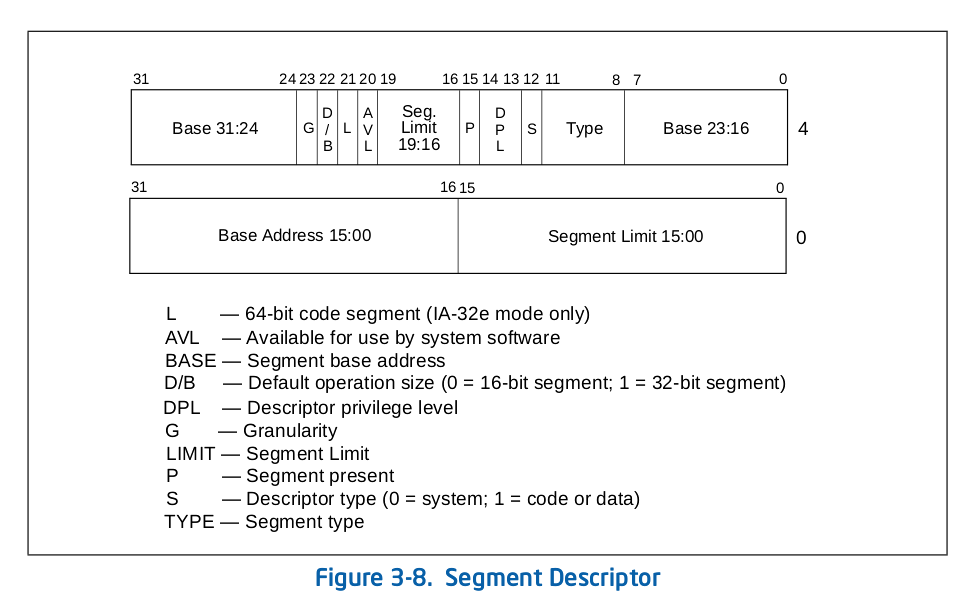
\includegraphics[scale=0.45]{picture/chapt6/segment_descriptor.png}
      \caption{段描述符的结构}
\end{figure}

 \par 显然,寄存器不足以存放N多个内存段的描述符集合,所以这些描述符的集合(称之为描述符表)被放置在内存里了。 在很多描述符表中,最重要的就是所谓的全局描述符表(Global Descriptor Table,GDT),它为整个软硬件系统服务。

 \par 一个问题解决了,但是又引出了的其他问题。问题一:这些描述符表放置在内存哪里?答案是没有固定的位置,可以任由 程序员安排在任意合适的位置。问题一带出了问题二:既然没有指定固定位置,CPU如何知道全局描述符表在哪?答案是Intel干脆设置了 一个48位的专用的全局描述符表寄存器(GDTR)来保存全局描述符表的信息。那这48位怎么分配呢?如图所示,0-15位表示GDT 的边界位置(数值为表的长度-1,因为从0计算),16-47位(这32位)存放的就是GDT的基地址(恰似数组的首地址)。

\begin{figure}[ht]
      \centering
      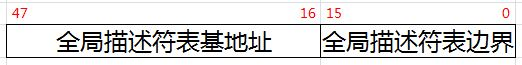
\includegraphics[scale=0.5]{picture/chapt6/gdtr.png}
      \caption{GDTR的结构}
\end{figure}

\par 既然用16位来表示表的长度,那么2的16次方就是65536字节,除以每一个描述符的8字节,那么最多能创建8192个描述符。

\par 貌似说了这么多,我们一直还没提CPU的默认工作方式。80386CPU加电的时候自动进入实模式\footnote{实际上此时CPU还不是彻底的实模式,之后第二条指令才进入彻底的实模式。对这个问题的讨论超出本文档的范围,所以不再讨论。}既然CPU加电后就一直工作在实模式下了。那怎么进入保护模式呢?说来也简单,80386CPU内部有5个32位的控制寄存器(Control Register,CR),分别是CR0到CR3,以及CR8。用来表示CPU的一些状态,其中的CR0寄存器的PE位(Protection Enable,保护模式允许位),0号位,就表示了CPU的运行状态,0为实模式,1为保护模式。通过修改这个位就可以立即改变CPU的工作模式。

\begin{figure}[ht]
      \centering
      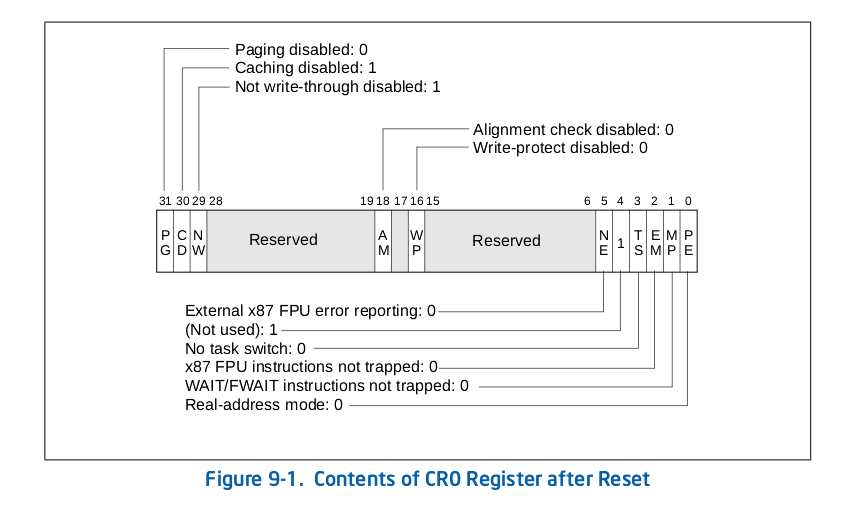
\includegraphics[scale=0.5]{picture/chapt6/cr0.png}
      \caption{CR0寄存器的结构}
\end{figure}

\par 不过需要注意的是,一旦CR0寄存器的PE位被修改,CPU就立即按照保护模式去寻址了,所以这就要求我们必须在进入保护模式之前就在内存里放置好GDT,然后设置好GDTR寄存器。我们知道实模式下只有1MB的寻址空间,所以GDT就等于被限制在了这里。即便是再不乐意我们也没有办法,只得委屈求全的先安排在这里。不过进入保护模式之后我们就可以在4G的空间里设置并修改原来的GDTR了。

\par OK,现在有了描述符的数组了,也有了“数组指针”(GDTR)了,怎么表示我们要访问哪个段呢?还记得8086时代的段寄存器吧?不过此时它们改名字了,叫段选择器(段选择子)。此时的CS等寄存器不再保存段基址了,而是保存其指向段的索引信息,CPU会根据这些信息在内存中获取到段信息。

\par 地址合成的过程如下图所示:

\begin{figure}[ht]
      \centering
      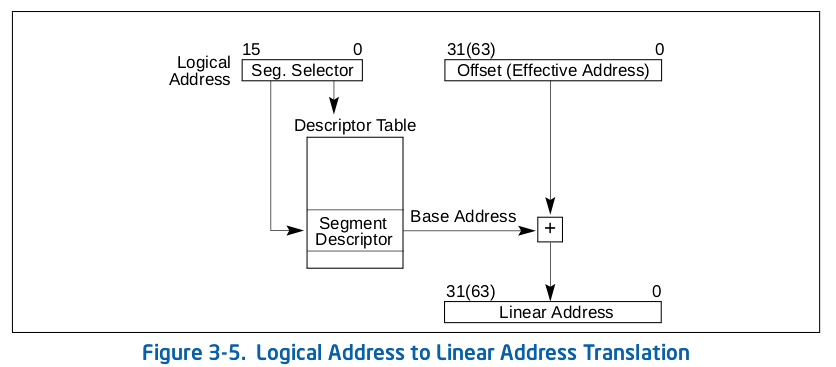
\includegraphics[scale=0.5]{picture/chapt6/protected_segment_addr.png}
      \caption{段机制的地址合成过程}
\end{figure}

\par 以上就是对x86保护模式的阐述了,细节问题希望大家能结合之后的代码自行参考Intel文档学习。

\subsection{具体采用的分段策略}

\par 下面开始针对我们的内核给出具体的设计方案了。我们之前简单的阐述了分段,事实上现代操作系统几乎不再使用分段而是绕过分段技术直接使用了分页。其实分段和分页没什么必然联系。只不过Intel从8086开始,其制造的CPU就以段地址+偏移地址的方式来访问内存。后来要兼容以前的CPU,Intel不得不一直保留着这个传统。分段可以说是Intel的CPU一直保持着的一种机制,而分页只是保护模式下的一种内存管理策略。不过想开启分页机制,CPU就必须工作在保护模式,而工作在保护模式时候可以不开启分页。所以事实上分段是必须的,而分页是可选的。

\par 那我们如何"绕过"这个分段机制呢?不知道大家是否还记得之前我们所说的平坦模式(Flat Mode)?这就是我们"绕过"的方法。当整个虚拟地址空间是一个起始地址为0,限长为4G的"段"时,我们给出的偏移地址在数值上等于段机制处理之后的地址了。
不过我们不是简单的对所有的段使用同样的描述符,而是给代码段和数据段分配不同的描述符。下面的示意图描述了这个抽象:

\begin{figure}[ht]
      \centering
      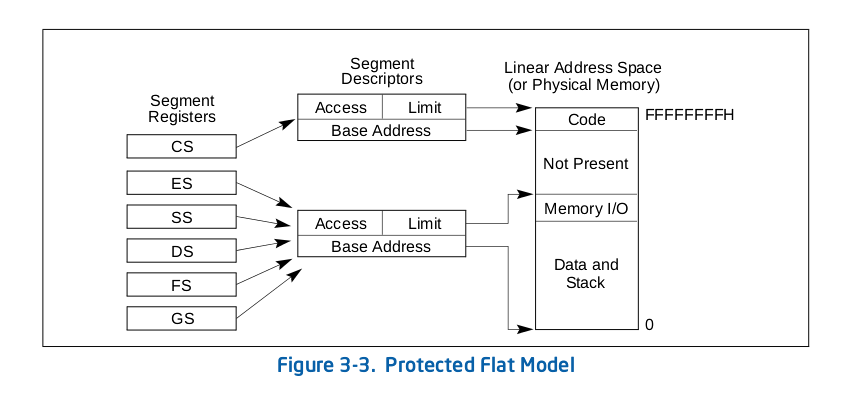
\includegraphics[scale=0.5]{picture/chapt6/protected_flat_mode.png}
      \caption{带有保护的平坦模式}
\end{figure}

\par 在第三章中我们谈到了GRUB在载入内核时候的一些状态,其中就有以下两条:

\begin{mdframed}
	\begin{enumerate}
		\item CS 指向基地址为 0x00000000,限长为4G – 1的代码段描述符。
		\item DS,SS,ES,FS 和 GS 指向基地址为0x00000000,限长为4G–1的数据段描述符。
	\end{enumerate}
\end{mdframed}

\par 大家现在应该理解这两项了吧?既然GRUB已经替我们做过了,那我们还有必要再来一次吗?当然有必要了,一来是学习的必要,二来在后期实现TSS任务切换的时候还要用到全局描述符表。

\par 下面我们给出具体的实现代码,首先是头文件和一些定义:

\begin{lstlisting}[language = C, caption = include/gdt.h]
#ifndef INCLUDE_GDT_H_
#define INCLUDE_GDT_H_

#include "types.h"

// 全局描述符类型
typedef
struct gdt_entry_t {
	uint16_t limit_low;     // 段界限   15 ~ 0
	uint16_t base_low;      // 段基地址 15 ~ 0
	uint8_t  base_middle;   // 段基地址 23 ~ 16
	uint8_t  access;        // 段存在位、描述符特权级、描述符类型、描述符子类别
	uint8_t  granularity; 	// 其他标志、段界限 19 ~ 16
	uint8_t  base_high;     // 段基地址 31 ~ 24
} __attribute__((packed)) gdt_entry_t;

// GDTR
typedef
struct gdt_ptr_t {
	uint16_t limit; 	// 全局描述符表限长
	uint32_t base; 		// 全局描述符表 32 位基地址
} __attribute__((packed)) gdt_ptr_t;

// 初始化全局描述符表
void init_gdt();

// GDT 加载到 GDTR 的函数[汇编实现]
extern void gdt_flush(uint32_t);

#endif 	// INCLUDE_GDT_H_
\end{lstlisting}

\par 结合上面关于全局段描述符表的格式说明,这两个结构体的定义应该很容易看懂。具体的函数实现如下:

\begin{lstlisting}[language = C, caption = gdt/gdt.c]
#include "gdt.h"
#include "string.h"

// 全局描述符表长度
#define GDT_LENGTH 5

// 全局描述符表定义
gdt_entry_t gdt_entries[GDT_LENGTH];

// GDTR
gdt_ptr_t gdt_ptr;

static void gdt_set_gate(int32_t num, uint32_t base,
			uint32_t limit, uint8_t access, uint8_t gran);

// 声明内核栈地址
extern uint32_t stack;

// 初始化全局描述符表
void init_gdt()
{
	// 全局描述符表界限 e.g. 从 0 开始,所以总长要 - 1
	gdt_ptr.limit = sizeof(gdt_entry_t) * GDT_LENGTH - 1;
	gdt_ptr.base = (uint32_t)&gdt_entries;

	// 采用 Intel 平坦模型
	gdt_set_gate(0, 0, 0, 0, 0);   // 按照 Intel 文档要求,第一个描述符必须全 0
	gdt_set_gate(1, 0, 0xFFFFFFFF, 0x9A, 0xCF); 	// 指令段
	gdt_set_gate(2, 0, 0xFFFFFFFF, 0x92, 0xCF); 	// 数据段
	gdt_set_gate(3, 0, 0xFFFFFFFF, 0xFA, 0xCF); 	// 用户模式代码段
	gdt_set_gate(4, 0, 0xFFFFFFFF, 0xF2, 0xCF); 	// 用户模式数据段

	// 加载全局描述符表地址到 GPTR 寄存器
	gdt_flush((uint32_t)&gdt_ptr);
}

// 全局描述符表构造函数,根据下标构造
// 参数分别是 数组下标、基地址、限长、访问标志,其它访问标志
static void gdt_set_gate(int32_t num, uint32_t base, uint32_t limit, uint8_t access, uint8_t gran)
{
	gdt_entries[num].base_low     = (base & 0xFFFF);
	gdt_entries[num].base_middle  = (base >> 16) & 0xFF;
	gdt_entries[num].base_high    = (base >> 24) & 0xFF;

	gdt_entries[num].limit_low    = (limit & 0xFFFF);
	gdt_entries[num].granularity  = (limit >> 16) & 0x0F;

	gdt_entries[num].granularity |= gran & 0xF0;
	gdt_entries[num].access       = access;
}

\end{lstlisting}

\par 这里唯一麻烦的就是需要对照着Intel文档的说明,为每一个段描述符计算权限位的数值了。至于加载全局描述符表的操作,方便起见我们直接用汇编语言实现了,代码如下:\footnote{这里需要强调的是这里的代码文件命名为gdt\_s.s,因为同一个目录下的.s和.c文件都会被编译为同名的.o文件,所以同名的话会被相互覆盖掉。}

\begin{lstlisting}[language = {[x86masm]Assembler}, caption = gdt/gdt\_s.s]
[GLOBAL gdt_flush]

gdt_flush:
	mov eax, [esp+4]  ; 参数存入 eax 寄存器
	lgdt [eax]        ; 加载到 GDTR [修改原先GRUB设置]

	mov ax, 0x10      ; 加载我们的数据段描述符
	mov ds, ax        ; 更新所有可以更新的段寄存器
	mov es, ax
	mov fs, ax
	mov gs, ax
	mov ss, ax
	jmp 0x08:.flush   ; 远跳转, 0x08 是我们的代码段描述符
			  ; 远跳目的是清空流水线并串行化处理器
.flush:
	ret
\end{lstlisting}

\par 我想这个汇编函数中唯一需要解释的就是jmp跳转那一句了,首先0×08是我们跳转目标段的段选择子(这个不陌生吧?),其对应段描述符第2项。后面的跳转目标标号可能会让你诧异,因为它就是下一行代码。这是为何?当然有深意了,第一,Intel不允许直接修改段寄存器cs的值,我们只好这样通过这种方式更新cs段寄存器;第二,x86以后CPU所增加的指令流水线和高速缓存可能会在新的全局描述符表加载之后依旧保持之前的缓存,那么修改GDTR之后最安全的做法就是立即清空流水线和更新高速缓存。说的这么牛逼的样子,其实只要一句jmp跳转就能强迫CPU自动更新了,很简单吧?

\par 到这里段描述符表的创建就告一段落了,其实我们完全可以直接计算出这些段具体的表示数值然后硬编码进去,但是出于学习的目的,我们还是写了这些函数进行处理。当然了,我们没有谈及一些具体的描述符细节问题,因为Intel文档的描述都很详细。

\par 创建好所有的文件以后,再次修改入口函数如下:

\begin{lstlisting}[language = C, caption = init/entry.c]
#include "gdt.h"
#include "console.h"
#include "debug.h"

int kern_entry()
{
	init_debug();
	init_gdt();

	console_clear();
	printk_color(rc_black, rc_green, "Hello, OS kernel!\n");

	return 0;
}
\end{lstlisting}

\par 编译运行后如果输出了正常的信息,就说明我们成功了。于是,本章结束。

% 第7章
% -*- coding: UTF-8 -*-
% hurlex-chapt7.tex
% hurlex 开发文档 第7章内容

\section {添加中断描述符表}

\subsection{中断的引入}

\par 中断是用以提高计算机工作效率、增强计算机功能的一项重要技术。其实简单说中断就是一种通知机制罢了。我们知道操作系统的一个核心任务就是和连接在主板上的所有的硬件设备进行通信,但是CPU和这些外设的速率根本就不在一个数量级上,倘若CPU向某一个设备发出一个请求并且一直等待反馈结果的话,这样带来的性能损失是不可接受的。而且CPU在运行期间需要得知外设所发生的事件,轮询显然是不可取的,那么就迫切需要一种机制来帮助我们解决这个问题。

\par 肩负着这一伟大使命,中断应运而生。当某个中断发生时,典型的处理方式就是CPU会打断当前的任务,保留当前的执行现场后再转移到该中断事先安排好的中断处理函数\footnote{或者叫中断服务例程。}去执行。在中断处理函数执行结束之后再恢复中断之前的执行现场,去执行之前的任务。

\par 从物理学的角度看,中断其实就是一种电信号,一般由硬件设备生成并送入中断控制器统一协调\footnote{当然需要一个"协调机构"了,\allowbreak\
试想所有设备不区分轻重缓急的和CPU发送中断信号的恐怖场景…}。中断控制器就是个简单的电子芯片,其作用就是将汇集的多路中断管线,采用复用技术只通过一条中断线和CPU相连接。既然中断控制器这里只有一条线和CPU相链接,那么为了区分各个设备,中断自然就有编号了。

\par 补充一下,其实CPU的中断管脚并非只有一根,其实是有NMI和INTR两个管脚,因为从严重性上来看,中断是分为两类的,首先NMI管脚触发的中断是需要无条件立即处理的,这种类型的中断是不会被阻塞和屏蔽的,所以叫做非屏蔽中断(Non Maskable Interrupt, NMI)。事实上一旦产生了NMI中断,就意味着CPU遇到了不可挽回的错误,一般不会进行处理,只是给出一个错误信息。而我们之前所说的中断控制器连接的管脚叫做INTR,这类中断有两个特点,分别是数量多和可屏蔽。而我们主要关注的正是INTR中断。

\par 举一个通俗的例子,假设你就是CPU,你正在看书(执行任务),突然间你的鼻涕流下来了(一个NMI中断),这个自然是不可以屏蔽的,不然会流到嘴里的…(好恶心),你现在把书反着扣在桌子上避免找不到页码(保留当前执行现场),取出纸巾…(此处省略几十个字),OK,你处理完后把书拿起来继续看(恢复之前的执行现场)。这就是一个中断的处理过程,其实很简单是不是?这是不可屏蔽中断,那么可屏蔽的呢?还是刚刚那个场景,你在看书,手机响了(一个INTR中断),但是你在学习期间不想被打扰,就无视它了…这就是可屏蔽中断了。

\par 通俗的例子举完了,我们还是专业一点好了。在x86PC中,我们熟知的中断控制芯片就是8259A PIC了,它就是我们说的中断控制器了。Intel的处理器允许256个中断,中断号范围是0~255。8259A PIC芯片负责15个,但是并不固定中断号,允许通过IO端口设置以避免冲突。它的全称是可编程中断控制器(Programmable Interrupt Controller,PIC)。关于8259A PIC的资料网上铺天盖地的,至于8259A PIC的结构,如何屏蔽中断什么的我就不多说了,请大家自行去了解。

\par 其实从上面的描述中我们基本上能理解中断的概念了。再简单说就是硬件发生了某个事件后告诉中断控制器,中断控制器汇报给CPU,CPU从中断控制器处得知了中断号,根据这个中断号找到对应的中断处理程序并转移过去执行,完成后重新回到之前的执行流程去。

\par 我们之前一直说的都是硬件中断,其实除了硬件中断之外还有软件中断,也就是软件系统也可以利用中断机制来完成一些任务,比如有些OS的系统调用的实现就采用了中断的方式。

\subsection{中断的实现}

\par 我们的重点是保护模式下的中断处理。中断处理程序是运行在ring0层的,这就意味着中断处理程序拥有着系统的全部权限,仿照内存段描述符表的思路,Intel设置了一个叫做中断描述符表(IDT, Interrupt Descriptor Table)的东西,和段描述符表一样放置在主存中,类似地,也有一个中断描述符表寄存器(IDTR)记录这个表的起始地址。那么下文的重点就是这个中断描述符的结构和设置方法了,其实这里很类似GDT的那一套过程,我们先给出中断描述符表的结构:\footnote{照例引用Intel文档中的插图,这是一篇开源的文档,应该没有版权纠纷吧...}

\begin{figure}[ht]
      \centering
      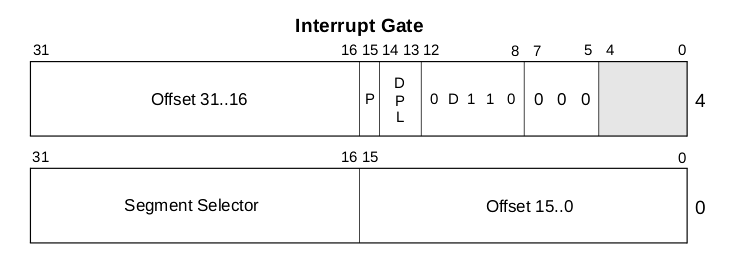
\includegraphics[scale=0.5]{picture/chapt7/interrupt_gate.png}
      \caption{中断描述符的格式}
\end{figure}

\par 根据这个描述信息,我们给出相关的C语言结构体定义:

\begin{lstlisting}[language = C, caption = include/idt.h]
#ifndef INCLUDE_IDT_H_
#define INCLUDE_IDT_H_

#include "types.h"

// 初始化中断描述符表
void init_idt();

// 中断描述符
typedef
struct idt_entry_t {
	uint16_t base_lo;        // 中断处理函数地址 15 ~ 0 位
	uint16_t sel;            // 目标代码段描述符选择子
	uint8_t  always0;        // 置 0 段
	uint8_t  flags;          // 一些标志,文档有解释
	uint16_t base_hi;        // 中断处理函数地址 31 ~ 16 位
}__attribute__((packed)) idt_entry_t;

// IDTR
typedef
struct idt_ptr_t {
	uint16_t limit; 	// 限长
	uint32_t base; 		// 基址
} __attribute__((packed)) idt_ptr_t;

#endif 	// INCLUDE_IDT_H_
\end{lstlisting}

\par 之前我们建立了中断的概念并且介绍了描述符表的结构,接下来我们细化CPU处理中断的过程,首先是起始过程,也就是从CPU发现中断事件后,打断当前程序或任务的执行,根据某种机制跳转到中断处理函数去执行的过程:
\begin{enumerate}
	\item CPU在执行完当前程序的每一条指令后,都会去确认在执行刚才的指令过程中是否发送中断请求过来,如果有,那么CPU		就会在相应的时钟脉冲到来时从总线上读取中断请求对应的中断向量。然后根据得到的中断向量为索引,到IDT中找到该向量		对应的中断描述符,中断描述符里保存着中断处理函数的段选择子;
	\item CPU根据IDT查到的中断处理函数段选择子,从GDT中取得相应的段描述符,段描述符里保存了中断处理函数的段基址和属性信息。		此时CPU要进行一个很关键的特权检验的过程,这个涉及到CPL、RPL和DPL的数值检验以及判断是否发生用户态到内核态的切换。		如果发生了切换,还要涉及到TSS段和用户栈和内核栈的切换;\footnote{这些东西我们之前都没有说过,所以大家看不懂的话		就先跳过去,等到后面讲到保护环的时候我们再细说。}
	\item 确认无误后CPU开始保存当前被打断的程序的现场(即一些寄存器的值),以便于将来恢复被打断的程序继续执行。这需要利用内核栈来保存		相关现场信息,即依次压入当前被打断程序使用的eflags、cs、eip、以及错误代码号(如果当前中断有错误代码);
	\item 最后CPU会从中断描述符中取出中断处理函数的起始地址并跳转过去执行。
\end{enumerate}

\par 以上是起始过程,中断处理函数执行完成之后需要通过iret或iretd指令恢复被打断的程序的执行。这时候比较简单,首先CPU会从内核栈里弹出先前保存的被打断的程序的现场信息,即之前的eflags,cs,eip重新开始被打断前的任务。\footnote{如果之前存在特权级转换(从内核态转换到用户态),则还需要从内核栈中弹出用户态栈的ss和esp,这样也意味着栈也被切换回原先使用的用户态的栈了。}
\par 需要注意的是:如果此次处理的是带有错误码的中断,CPU 在恢复先前程序的现场时,并不会弹出错误代码。这一步需要通过软件完成,即要求相关的中断处理函数在使用iret指令返回之前添加出栈代码主动弹出错误代码。

\par 下图描述了CPU自动保护和恢复的寄存器的栈结构:
\begin{figure}[ht]
      \centering
      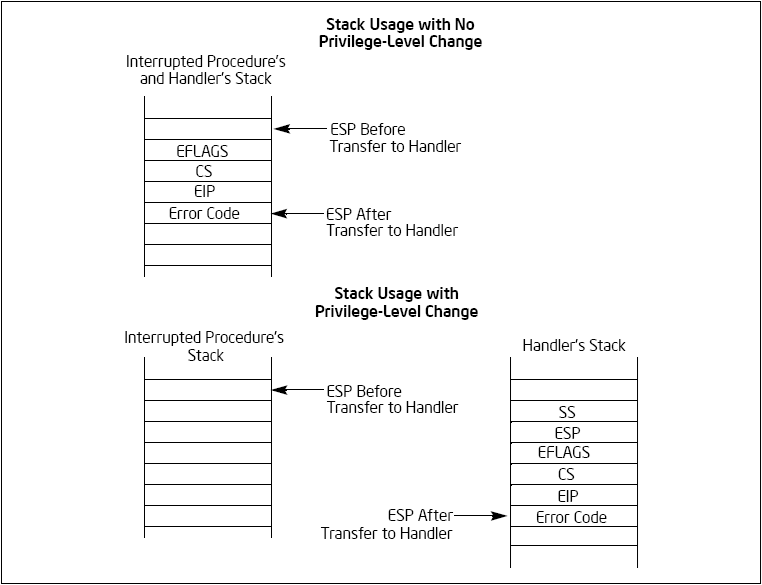
\includegraphics[scale=0.4]{picture/chapt7/interrupt_stack.png}
      \caption{中断发生时CPU保存的现场}
\end{figure}

\par CPU在发生中断的时候是按照上文所描述的过程执行的,那操作系统需要做什么呢?

\par 首先是实现中断处理函数。按照Intel的规定,0~19号中断属于CPU所有\footnote{这些由CPU自身产生的中断也被称之为异常。},而且第20-31号中断也被Intel保留,所以从32~255号才属于用户自定义中断。虽说是"用户自定义",其实在x86上有些中断按照习惯还是给予了固定的设备。比如32号是timer中断,33号是键盘中断等等。

\par 中断处理函数怎么实现呢?直接可以进行相关的逻辑处理吗?当然不行了。CPU在中断产生时自动保存了部分的执行现场,但是依旧有很多寄存器需要我们自己去保护和恢复,下面是CPU保护的寄存器和剩余需要保护的寄存器一起定义的结构体。

\begin{lstlisting}[language = C, caption = include/idt.h]
// 寄存器类型
typedef
struct pt_regs_t {
	uint32_t ds; 		// 用于保存用户的数据段描述符
	uint32_t edi; 		// 从 edi 到 eax 由 pusha 指令压入
	uint32_t esi; 
	uint32_t ebp;
	uint32_t esp;
	uint32_t ebx;
	uint32_t edx;
	uint32_t ecx;
	uint32_t eax;
	uint32_t int_no; 	// 中断号
	uint32_t err_code;  	// 错误代码(有中断错误代码的中断会由CPU压入)
	uint32_t eip; 		// 以下由处理器自动压入
	uint32_t cs; 		
	uint32_t eflags;
	uint32_t useresp;
	uint32_t ss;
} pt_regs;

// 定义中断处理函数指针
typedef void (*interrupt_handler_t)(pt_regs *);

// 注册一个中断处理函数
void register_interrupt_handler(uint8_t n, interrupt_handler_t h);

// 调用中断处理函数
void isr_handler(pt_regs *regs);

// 声明中断处理函数 0 ~ 19 属于 CPU 的异常中断
// ISR:中断服务程序(interrupt service routine)
void isr0(); 		// 0 #DE 除 0 异常 
void isr1(); 		// 1 #DB 调试异常 
void isr2(); 		// 2 NMI 
void isr3(); 		// 3 BP 断点异常 
void isr4(); 		// 4 #OF 溢出 
void isr5(); 		// 5 #BR 对数组的引用超出边界 
void isr6(); 		// 6 #UD 无效或未定义的操作码 
void isr7(); 		// 7 #NM 设备不可用(无数学协处理器) 
void isr8(); 		// 8 #DF 双重故障(有错误代码) 
void isr9(); 		// 9 协处理器跨段操作 
void isr10(); 		// 10 #TS 无效TSS(有错误代码) 
void isr11(); 		// 11 #NP 段不存在(有错误代码) 
void isr12(); 		// 12 #SS 栈错误(有错误代码) 
void isr13(); 		// 13 #GP 常规保护(有错误代码) 
void isr14(); 		// 14 #PF 页故障(有错误代码) 
void isr15(); 		// 15 CPU 保留 
void isr16(); 		// 16 #MF 浮点处理单元错误 
void isr17(); 		// 17 #AC 对齐检查 
void isr18(); 		// 18 #MC 机器检查 
void isr19(); 		// 19 #XM SIMD(单指令多数据)浮点异常

// 20 ~ 31 Intel 保留
void isr20();
void isr21();
void isr22();
void isr23();
void isr24();
void isr25();
void isr26();
void isr27();
void isr28();
void isr29();
void isr30();
void isr31();

// 32 ~ 255 用户自定义异常
void isr255();
\end{lstlisting}

\par 一个很现实的问题是:所有的中断处理函数中,除了CPU本身保护的现场外,其它寄存器的保存和恢复过程都是一样的。所以,如果在每个中断处理函数中都实现一次显然冗余而且易错。所以我们很自然把原本的中断处理函数逻辑上拆解为三部分,第一部分是一致的现场保护操作;第二部分是每个中断特有的处理逻辑;第三部分又是一致的现场恢复。

\par 实际上我们把每个中断处理函数拆解为四段,在四个函数里实现。具体的实现如下:

\begin{lstlisting}[language = {[x86masm]Assembler}, caption = idt/idt\_s.s]
; 定义两个构造中断处理函数的宏(有的中断有错误代码,有的没有)
; 用于没有错误代码的中断
%macro ISR_NOERRCODE 1
[GLOBAL isr%1]
isr%1:
	cli                  ; 首先关闭中断
	push 0               ; push 无效的中断错误代码
	push %1              ; push 中断号
	jmp isr_common_stub
%endmacro

; 用于有错误代码的中断
%macro ISR_ERRCODE 1
[GLOBAL isr%1]
isr%1:
	cli                  ; 关闭中断
	push %1              ; push 中断号
	jmp isr_common_stub
%endmacro

; 定义中断处理函数
ISR_NOERRCODE  0 	; 0 #DE 除 0 异常
ISR_NOERRCODE  1 	; 1 #DB 调试异常
ISR_NOERRCODE  2 	; 2 NMI
ISR_NOERRCODE  3 	; 3 BP 断点异常 
ISR_NOERRCODE  4 	; 4 #OF 溢出 
ISR_NOERRCODE  5 	; 5 #BR 对数组的引用超出边界 
ISR_NOERRCODE  6 	; 6 #UD 无效或未定义的操作码 
ISR_NOERRCODE  7 	; 7 #NM 设备不可用(无数学协处理器) 
ISR_ERRCODE    8 	; 8 #DF 双重故障(有错误代码) 
ISR_NOERRCODE  9 	; 9 协处理器跨段操作
ISR_ERRCODE   10 	; 10 #TS 无效TSS(有错误代码) 
ISR_ERRCODE   11 	; 11 #NP 段不存在(有错误代码) 
ISR_ERRCODE   12 	; 12 #SS 栈错误(有错误代码) 
ISR_ERRCODE   13 	; 13 #GP 常规保护(有错误代码) 
ISR_ERRCODE   14 	; 14 #PF 页故障(有错误代码) 
ISR_NOERRCODE 15 	; 15 CPU 保留 
ISR_NOERRCODE 16 	; 16 #MF 浮点处理单元错误 
ISR_ERRCODE   17 	; 17 #AC 对齐检查 
ISR_NOERRCODE 18 	; 18 #MC 机器检查 
ISR_NOERRCODE 19 	; 19 #XM SIMD(单指令多数据)浮点异常

; 20 ~ 31 Intel 保留
ISR_NOERRCODE 20
ISR_NOERRCODE 21
ISR_NOERRCODE 22
ISR_NOERRCODE 23
ISR_NOERRCODE 24
ISR_NOERRCODE 25
ISR_NOERRCODE 26
ISR_NOERRCODE 27
ISR_NOERRCODE 28
ISR_NOERRCODE 29
ISR_NOERRCODE 30
ISR_NOERRCODE 31
; 32 ~ 255 用户自定义
ISR_NOERRCODE 255
\end{lstlisting}

\par 函数执行的开始位置我们自行向栈里压入中断的号码,这是为了识别出中断号码。上面的代码用到了NASM的宏汇编,因为指令结构是相同的,所以我们可以用宏汇编来生成代码。如果大家对这里有疑问的话,可以参考NASM手册或者直接对生成的内核文件反汇编查看相关函数的实现。另外还有一点需要说明的是,因为有的中断处理函数会自动压入错误号,而有的不会,这样给我们的清栈造成了麻烦。所以我们在不会压入错误号的中断的处理函数里手动压入0作为占位,这样方便我们在清理的时候不用分类处理。

\par 以上是中断处理函数的最前一部分,接下来是所有中断处理函数共有的保护现场操作:
\begin{lstlisting}[language = {[x86masm]Assembler}, caption = idt/idt\_s.s]
[GLOBAL isr_common_stub]
[EXTERN isr_handler]
; 中断服务程序
isr_common_stub:
	pusha                    ; Pushes edi, esi, ebp, esp, ebx, edx, ecx, eax
	mov ax, ds
	push eax                ; 保存数据段描述符
	
	mov ax, 0x10            ; 加载内核数据段描述符表
	mov ds, ax
	mov es, ax
	mov fs, ax
	mov gs, ax
	mov ss, ax
	
	push esp		; 此时的 esp 寄存器的值等价于 pt_regs 结构体的指针
	call isr_handler        ; 在 C 语言代码里
	add esp, 4 		; 清除压入的参数
	
	pop ebx                 ; 恢复原来的数据段描述符
	mov ds, bx
	mov es, bx
	mov fs, bx
	mov gs, bx
	mov ss, bx
	
	popa                     ; Pops edi, esi, ebp, esp, ebx, edx, ecx, eax
	add esp, 8               ; 清理栈里的 error code 和 ISR
	iret
.end:
\end{lstlisting}

\par 这里声明了一个外部函数isr\_handler,它的实现如下:
\begin{lstlisting}[language = C, caption = idt/idt.c]
// 调用中断处理函数
void isr_handler(pt_regs *regs)
{
	if (interrupt_handlers[regs->int_no]) {
	      interrupt_handlers[regs->int_no](regs);
	} else {
		printk_color(rc_black, rc_blue, "Unhandled interrupt: %d\n", regs->int_no);
	}
}
\end{lstlisting}

\par 从上面的代码中我们看到,事实上具体的中断处理函数的原型都是 void (pt\_regs *),它们被统一组织放置在全局的函数指针数组interrupt\_handers里面。isr\_hanlder函数,如判断这个中断函数是否注册,如果注册了会执行该函数,否则打印出Unhandled interrupt和中断号码。

\par 最后是中断描述符表的创建和加载函数:
\begin{lstlisting}[language = C, caption = idt/idt.c]
#include "common.h"
#include "string.h"
#include "debug.h"
#include "idt.h"

// 中断描述符表
idt_entry_t idt_entries[256];

// IDTR
idt_ptr_t idt_ptr;

// 中断处理函数的指针数组
interrupt_handler_t interrupt_handlers[256];

// 设置中断描述符
static void idt_set_gate(uint8_t num, uint32_t base, uint16_t sel, uint8_t flags);

// 声明加载 IDTR 的函数
extern void idt_flush(uint32_t);

// 初始化中断描述符表
void init_idt()
{	
	bzero((uint8_t *)&interrupt_handlers, sizeof(interrupt_handler_t) * 256);
	
	idt_ptr.limit = sizeof(idt_entry_t) * 256 - 1;
	idt_ptr.base  = (uint32_t)&idt_entries;
	
	bzero((uint8_t *)&idt_entries, sizeof(idt_entry_t) * 256);

	// 0-32:  用于 CPU 的中断处理
	idt_set_gate( 0, (uint32_t)isr0,  0x08, 0x8E);
	idt_set_gate( 1, (uint32_t)isr1,  0x08, 0x8E);
	idt_set_gate( 2, (uint32_t)isr2,  0x08, 0x8E);
	idt_set_gate( 3, (uint32_t)isr3,  0x08, 0x8E);
	idt_set_gate( 4, (uint32_t)isr4,  0x08, 0x8E);
	idt_set_gate( 5, (uint32_t)isr5,  0x08, 0x8E);
	idt_set_gate( 6, (uint32_t)isr6,  0x08, 0x8E);
	idt_set_gate( 7, (uint32_t)isr7,  0x08, 0x8E);
	idt_set_gate( 8, (uint32_t)isr8,  0x08, 0x8E);
	idt_set_gate( 9, (uint32_t)isr9,  0x08, 0x8E);
	idt_set_gate(10, (uint32_t)isr10, 0x08, 0x8E);
	idt_set_gate(11, (uint32_t)isr11, 0x08, 0x8E);
	idt_set_gate(12, (uint32_t)isr12, 0x08, 0x8E);
	idt_set_gate(13, (uint32_t)isr13, 0x08, 0x8E);
	idt_set_gate(14, (uint32_t)isr14, 0x08, 0x8E);
	idt_set_gate(15, (uint32_t)isr15, 0x08, 0x8E);
	idt_set_gate(16, (uint32_t)isr16, 0x08, 0x8E);
	idt_set_gate(17, (uint32_t)isr17, 0x08, 0x8E);
	idt_set_gate(18, (uint32_t)isr18, 0x08, 0x8E);
	idt_set_gate(19, (uint32_t)isr19, 0x08, 0x8E);
	idt_set_gate(20, (uint32_t)isr20, 0x08, 0x8E);
	idt_set_gate(21, (uint32_t)isr21, 0x08, 0x8E);
	idt_set_gate(22, (uint32_t)isr22, 0x08, 0x8E);
	idt_set_gate(23, (uint32_t)isr23, 0x08, 0x8E);
	idt_set_gate(24, (uint32_t)isr24, 0x08, 0x8E);
	idt_set_gate(25, (uint32_t)isr25, 0x08, 0x8E);
	idt_set_gate(26, (uint32_t)isr26, 0x08, 0x8E);
	idt_set_gate(27, (uint32_t)isr27, 0x08, 0x8E);
	idt_set_gate(28, (uint32_t)isr28, 0x08, 0x8E);
	idt_set_gate(29, (uint32_t)isr29, 0x08, 0x8E);
	idt_set_gate(30, (uint32_t)isr30, 0x08, 0x8E);
	idt_set_gate(31, (uint32_t)isr31, 0x08, 0x8E);

	// 255 将来用于实现系统调用
	idt_set_gate(255, (uint32_t)isr255, 0x08, 0x8E);

	// 更新设置中断描述符表
	idt_flush((uint32_t)&idt_ptr);
}

// 设置中断描述符
static void idt_set_gate(uint8_t num, uint32_t base, uint16_t sel, uint8_t flags)
{
	idt_entries[num].base_lo = base & 0xFFFF;
	idt_entries[num].base_hi = (base >> 16) & 0xFFFF;

	idt_entries[num].sel     = sel;
	idt_entries[num].always0 = 0;

	// 先留下 0x60 这个魔数,以后实现用户态时候
	// 这个与运算可以设置中断门的特权级别为 3
	idt_entries[num].flags = flags;  // | 0x60
}
\end{lstlisting}

\par 加载中断描述符表的函数很简单:
\begin{lstlisting}[language = {[x86masm]Assembler}, caption = idt/idt\_s.s]
[GLOBAL idt_flush]
idt_flush:
	mov eax, [esp+4]  ; 参数存入 eax 寄存器
	lidt [eax]        ; 加载到 IDTR
	ret
.end:
\end{lstlisting}

\par 整理好上面的代码,修改入口函数测试一下中断吧。入口代码修改如下:
\begin{lstlisting}[language = C, caption = init/entry.c]
#include "console.h"
#include "debug.h"
#include "gdt.h"
#include "idt.h"

int kern_entry()
{
	init_debug();
	init_gdt();
	init_idt();

	console_clear();
	printk_color(rc_black, rc_green, "Hello, OS kernel!\n");

	asm volatile ("int $0x3");
	asm volatile ("int $0x4");

	return 0;
}
\end{lstlisting}

\par 编译运行,我们得到了正确的结果:\footnote{当然了,我们没有注册具体的处理函数,所以就打印默认的信息了。}
\begin{figure}[ht]
      \centering
      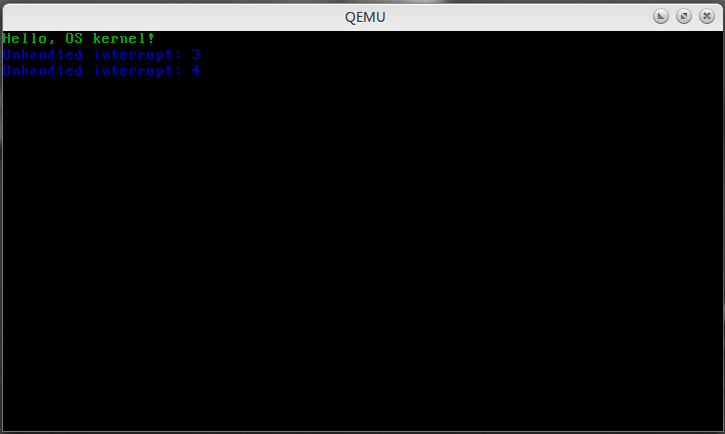
\includegraphics[scale=0.5]{picture/chapt7/interrupt_view.png}
      \caption{中断处理函数的测试}
\end{figure}

% 第8章
% -*- coding: UTF-8 -*-
% hurlex-chapt8.tex
% hurlex 开发文档 第8章内容

\section {完成中断请求和定时器中断}

\par 在上一章中我们完成了中断处理程序的框架,本章在其基础上讨论中断请求的实现。

\par 我们在上一章中提到,外设的所有中断由中断控制芯片8259A统一汇集之后连接到CPU的INTR引脚。\footnote{这里肯定会有读者提出来现代的计算机主板上早就使用APIC(Advanced Programmable Interrupt Controller,高级可编程中断控制器)来进行外设的中断管理了。没错,但是我相信在本科阶段的微机原理和接口技术中学的是8259APIC(Programmable Interrupt Controller),而且无论硬件怎么发展,始终会兼容以前的接口。本着大家熟悉易理解的原则,我们依旧使用兼容的8259APIC(Programmable Interrupt Controller, 可编程中断控制器)的设置方法进行设置。}这章我们就来探究8259APIC的初始化和实现定时器的中断处理。

\par 8259A PIC每一片可以管理8个中断源,显然一般情况下设备数量会超过这个值。这里就要提到IBM PC/AT 8259A PIC架构了,IBM的设计方案是使用8259APIC的级联功能,使用两片级联(分为主、从片)的方式来管理硬件中断。其中主片的INT端连接到CPU的INTR引脚,从片的INT连接到主片的IR2引脚。结构如下图所示:
\begin{figure}[ht]
      \centering
      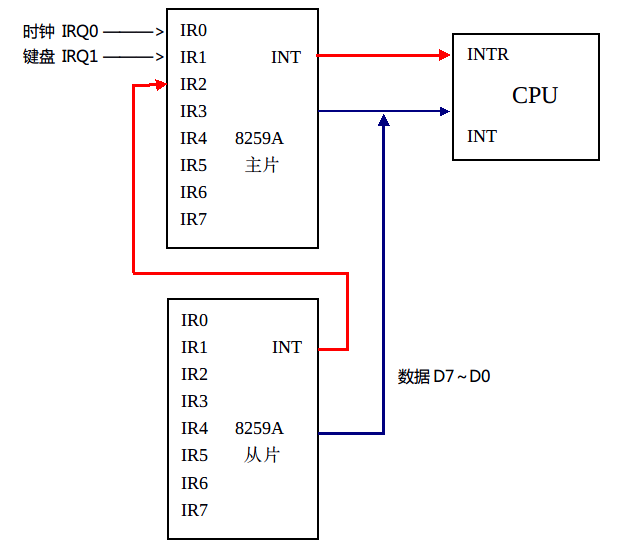
\includegraphics[scale=0.5]{picture/chapt8/8259A_PIC.png}
      \caption{8259A PIC级联}
\end{figure}

\par 图中时钟中断连接在主片的IRQ0引脚,键盘中断连接在了主片的IRQ1引脚。其它的引脚暂时用不到就不说了。在上一张描述中断描述符表时我们知道了0~31号中断是CPU使用和保留的,用户可以使用的中断从32号开始。所以这里的IRQ0对应的中断号就是32号,IRQ1就是33号,然后以此类推。

\par 理论就暂时阐述到这里,接下来是实现代码。首先是对8259A PIC的初始化,在设置中断描述符表的函数init\_idt最前面加入如下代码:

\begin{lstlisting}[language = C, caption = idt/idt.c]
// 初始化中断描述符表
void init_idt()
{	
	// 重新映射 IRQ 表
	// 两片级联的 Intel 8259A 芯片
	// 主片端口 0x20 0x21
	// 从片端口 0xA0 0xA1
	
	// 初始化主片、从片
	// 0001 0001
	outb(0x20, 0x11);
	outb(0xA0, 0x11);

	// 设置主片 IRQ 从 0x20(32) 号中断开始
	outb(0x21, 0x20);

	// 设置从片 IRQ 从 0x28(40) 号中断开始
	outb(0xA1, 0x28);
	
	// 设置主片 IR2 引脚连接从片
	outb(0x21, 0x04);

	// 告诉从片输出引脚和主片 IR2 号相连
	outb(0xA1, 0x02);
	
	// 设置主片和从片按照 8086 的方式工作
	outb(0x21, 0x01);
	outb(0xA1, 0x01);
	
	// 设置主从片允许中断
	outb(0x21, 0x0);
	outb(0xA1, 0x0);
	
	... ...
}
\end{lstlisting}

\par 对8259A PIC具体的设置我们不再阐述,这种资料网上铺天盖地的都是。相信结合注释很容易理解这个简单的初始化过程。

\par 完成了初始化之后,我们继续添加对IRQ处理函数的添加。首先是在idt.h头文件末尾添加如下内容:

\begin{lstlisting}[language = C, caption = include/idt.h]
// IRQ 处理函数
void irq_handler(pt_regs *regs);

// 定义IRQ
#define  IRQ0     32 	// 电脑系统计时器
#define  IRQ1     33 	// 键盘
#define  IRQ2     34 	// 与 IRQ9 相接,MPU-401 MD 使用
#define  IRQ3     35 	// 串口设备
#define  IRQ4     36 	// 串口设备
#define  IRQ5     37 	// 建议声卡使用
#define  IRQ6     38 	// 软驱传输控制使用
#define  IRQ7     39 	// 打印机传输控制使用
#define  IRQ8     40 	// 即时时钟
#define  IRQ9     41 	// 与 IRQ2 相接,可设定给其他硬件
#define  IRQ10    42 	// 建议网卡使用
#define  IRQ11    43 	// 建议 AGP 显卡使用
#define  IRQ12    44 	// 接 PS/2 鼠标,也可设定给其他硬件
#define  IRQ13    45 	// 协处理器使用
#define  IRQ14    46 	// IDE0 传输控制使用
#define  IRQ15    47 	// IDE1 传输控制使用

// 声明 IRQ 函数
// IRQ:中断请求(Interrupt Request)
void irq0();		// 电脑系统计时器
void irq1(); 		// 键盘
void irq2(); 		// 与 IRQ9 相接,MPU-401 MD 使用
void irq3(); 		// 串口设备
void irq4(); 		// 串口设备
void irq5(); 		// 建议声卡使用
void irq6(); 		// 软驱传输控制使用
void irq7(); 		// 打印机传输控制使用
void irq8(); 		// 即时时钟
void irq9(); 		// 与 IRQ2 相接,可设定给其他硬件
void irq10(); 		// 建议网卡使用
void irq11(); 		// 建议 AGP 显卡使用
void irq12(); 		// 接 PS/2 鼠标,也可设定给其他硬件
void irq13(); 		// 协处理器使用
void irq14(); 		// IDE0 传输控制使用
void irq15(); 		// IDE1 传输控制使用
\end{lstlisting}

\par 然后是idt\_s.s中添加相应的处理过程:

\begin{lstlisting}[language = {[x86masm]Assembler}, caption = idt/idt\_s.s]
; 构造中断请求的宏
%macro IRQ 2
[GLOBAL irq%1]
irq%1:
	cli
	push byte 0
	push byte %2
	jmp irq_common_stub
%endmacro

IRQ   0,    32 	; 电脑系统计时器
IRQ   1,    33 	; 键盘
IRQ   2,    34 	; 与 IRQ9 相接,MPU-401 MD 使用
IRQ   3,    35 	; 串口设备
IRQ   4,    36 	; 串口设备
IRQ   5,    37 	; 建议声卡使用
IRQ   6,    38 	; 软驱传输控制使用
IRQ   7,    39 	; 打印机传输控制使用
IRQ   8,    40 	; 即时时钟
IRQ   9,    41 	; 与 IRQ2 相接,可设定给其他硬件
IRQ  10,    42 	; 建议网卡使用
IRQ  11,    43 	; 建议 AGP 显卡使用
IRQ  12,    44 	; 接 PS/2 鼠标,也可设定给其他硬件
IRQ  13,    45 	; 协处理器使用
IRQ  14,    46 	; IDE0 传输控制使用
IRQ  15,    47 	; IDE1 传输控制使用

[GLOBAL irq_common_stub]
[EXTERN irq_handler]
irq_common_stub:
	pusha                    ; pushes edi, esi, ebp, esp, ebx, edx, ecx, eax
	
	mov ax, ds
	push eax                 ; 保存数据段描述符
	
	mov ax, 0x10  		 ; 加载内核数据段描述符
	mov ds, ax
	mov es, ax
	mov fs, ax
	mov gs, ax
	mov ss, ax
	
	push esp
	call irq_handler
	add esp, 4
	
	pop ebx                   ; 恢复原来的数据段描述符
	mov ds, bx
	mov es, bx
	mov fs, bx
	mov gs, bx
	mov ss, bx
	
	popa                     ; Pops edi,esi,ebp...
	add esp, 8     		 ; 清理压栈的 错误代码 和 ISR 编号
	iret          		 ; 出栈 CS, EIP, EFLAGS, SS, ESP
.end:
\end{lstlisting}

\par 最后是init\_idt函数构造IRQ的相关描述符和具体的IRQ处理函数了。

\begin{lstlisting}[language = C, caption = idt/idt.c]
// 初始化中断描述符表
void init_idt()
{	
	... ...
	idt_set_gate(31, (uint32_t)isr31, 0x08, 0x8E);

	idt_set_gate(32, (uint32_t)irq0, 0x08, 0x8E);
	idt_set_gate(33, (uint32_t)irq1, 0x08, 0x8E);
	idt_set_gate(34, (uint32_t)irq2, 0x08, 0x8E);
	idt_set_gate(35, (uint32_t)irq3, 0x08, 0x8E);
	idt_set_gate(36, (uint32_t)irq4, 0x08, 0x8E);
	idt_set_gate(37, (uint32_t)irq5, 0x08, 0x8E);
	idt_set_gate(38, (uint32_t)irq6, 0x08, 0x8E);
	idt_set_gate(39, (uint32_t)irq7, 0x08, 0x8E);
	idt_set_gate(40, (uint32_t)irq8, 0x08, 0x8E);
	idt_set_gate(41, (uint32_t)irq9, 0x08, 0x8E);
	idt_set_gate(42, (uint32_t)irq10, 0x08, 0x8E);
	idt_set_gate(43, (uint32_t)irq11, 0x08, 0x8E);
	idt_set_gate(44, (uint32_t)irq12, 0x08, 0x8E);
	idt_set_gate(45, (uint32_t)irq13, 0x08, 0x8E);
	idt_set_gate(46, (uint32_t)irq14, 0x08, 0x8E);
	idt_set_gate(47, (uint32_t)irq15, 0x08, 0x8E);

	// 255 将来用于实现系统调用
	idt_set_gate(255, (uint32_t)isr255, 0x08, 0x8E);

	... ...
}

// IRQ 处理函数
void irq_handler(pt_regs *regs)
{
	// 发送中断结束信号给 PICs
	// 按照我们的设置,从 32 号中断起为用户自定义中断
	// 因为单片的 Intel 8259A 芯片只能处理 8 级中断
	// 故大于等于 40 的中断号是由从片处理的
	if (regs->int_no >= 40) {
		// 发送重设信号给从片
		outb(0xA0, 0x20);
	}
	// 发送重设信号给主片
	outb(0x20, 0x20);

	if (interrupt_handlers[regs->int_no]) {
		interrupt_handlers[regs->int_no](regs);
	}
}
\end{lstlisting}

\par 结合代码中详细的注释和本章开始的8259A PIC的结构图,详细很容易理解这个处理过程。其实IRQ和ISR的处理过程很类似:
\begin{mdframed}
	\begin{itemize}
		\item ISR的处理过程是 (isr0 - isr31) -> isr\_common\_stub -> isr\_handler -> 具体的ISR处理函数。
		\item IRQ的处理过程是 (irq0 - irq15) -> irq\_common\_stub -> irq\_hanlder -> 具体的IRQ处理函数。
	\end{itemize}
\end{mdframed}

\par 写到这里具体的IRQ处理过程就完成了,以后只需要设置好相应的处理函数就好了,接下来我们实现时钟中断的产生和处理。

\par 时钟中断对于操作系统内核来说,是很重要的一种中断,它使得CPU无论在执行任何用户或者内核的程序时,都能定时的将执行权利交还到CPU手中来。\footnote{当然了,屏蔽中断就没办法了。}除了记录时间之外,时钟中断的处理函数里通常都是对进程的调度处理。
\par 具体的时钟中断源是8253/8254 Timer 产成的,要按照需要的频率产生中断,需要先配置8253/8254 Timer芯片。代码如下:

\begin{lstlisting}[language = C, caption = drivers/timer.c]
#include "timer.h"
#include "debug.h"
#include "common.h"
#include "idt.h"

void timer_callback(pt_regs *regs)
{
	static uint32_t tick = 0;
	printk_color(rc_black, rc_red, "Tick: %d\n", tick++);
}

void init_timer(uint32_t frequency)
{
	// 注册时间相关的处理函数
	register_interrupt_handler(IRQ0, timer_callback);

	// Intel 8253/8254 PIT芯片 I/O端口地址范围是40h~43h
	// 输入频率为 1193180/frequency 即每秒中断次数
	uint32_t divisor = 1193180 / frequency;

	// D7 D6 D5 D4 D3 D2 D1 D0
	// 0  0  1  1  0  1  1  0
	// 即就是 36 H
	// 设置 8253/8254 芯片工作在模式 3 下
	outb(0x43, 0x36);

	// 拆分低字节和高字节
	uint8_t low = (uint8_t)(divisor & 0xFF);
	uint8_t hign = (uint8_t)((divisor >> 8) & 0xFF);
	
	// 分别写入低字节和高字节
	outb(0x40, low);
	outb(0x40, hign);
}
\end{lstlisting}

\par 对应的头文件如下:

\begin{lstlisting}[language = C, caption = include/timer.h]
#ifndef INCLUDE_TIMER_H_
#define INCLUDE_TIMER_H_

#include "types.h"

void init_timer(uint32_t frequency);

#endif 	// INCLUDE_TIMER_H_
\end{lstlisting}

\par 8253/8254 Timer有三种工作模式,我们使用第三种。init\_timer函数的参数是所需的时钟中断的频率,具体的设置原理不再赘述。最后,修改入口函数进行测试:

\begin{lstlisting}[language = C, caption = init/entry.c]
#include "console.h"
#include "debug.h"
#include "gdt.h"
#include "idt.h"
#include "timer.h"

int kern_entry()
{
	init_debug();
	init_gdt();
	init_idt();

	console_clear();
	printk_color(rc_black, rc_green, "Hello, OS kernel!\n");

	init_timer(200);

	// 开启中断
	asm volatile ("sti");

	return 0;
}

\end{lstlisting}

\par 最后编译执行,我们看到了如下的输出:
\begin{figure}[ht]
      \centering
      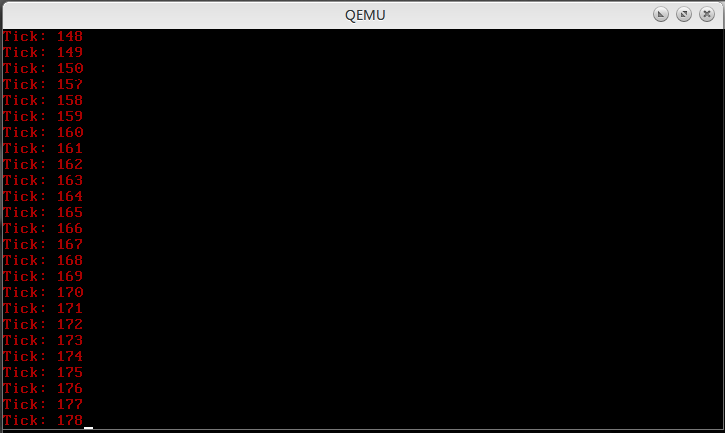
\includegraphics[scale=0.6]{picture/chapt8/8253_TIMER.png}
      \caption{8253/8254 Timer 中断}
\end{figure}


% 第9章
% -*- coding: UTF-8 -*-
% hurlex-chapt9.tex
% hurlex 开发文档 第9章内容

\section {物理内存管理的实现}

\par 这章我们来讨论操作系统内核的一个很重要的组成部分——内存管理模块。之前的章节中简单介绍了段式的内存管理,这章我们来讨论页式的内存管理。

\par 首先是CPU在保护模式下分页未开启和分页开启的不同状态时,MMU组件处理地址的流程。

\begin{mdframed}
	\begin{itemize}
		\item 如果没有开启分页:\\ 逻辑地址 -> 段机制处理 -> 线性地址 = 物理地址
		\item 如果开启分页:\\ 逻辑地址 -> 段机制处理 -> 线性地址 -> 页机制处理 -> 物理地址
	\end{itemize}
\end{mdframed}

\par 因为采用了平坦模式,所以给出的访问地址实际上已经等于线性地址了(段基址为0),那么剩下的问题就是所谓的页机制处理了。

\par 长时间以来,随着计算机技术的发展,存储器的容量在不断的高速增加着。但是说起内存(这里指RAM,下同)这个东西,它有一个很奇葩的特性,就是无论它有多大,都总是不够用(P.S.厨房的垃圾桶也一样)。现在我们看似拥有着以前的程序员想都不敢想的"天文数字"的内存,动辄就是几G十几G的。但是相信我,历史总是嘲弄人的。就像当年程序员们质疑32位地址线带来的4GB空间太大没有意义似的,我们也会有一天抱怨现在的内存太小的。

\par 那内存不够用了怎么办?还有,使用过程中出现的内存碎片怎么办?假设我们有4GB的物理内存,现在有1、2、3、4一共4个程序分别各占据连续的1G内存,然后2、4退出,此时虽然有空闲的两段内存,却连一个稍大于1GB的程序都无法载入了。

\par 当然了,这只是一个例子。不过按照一般的思路,在内存释放之后,如何回收呢?做碎片整理吗?即便我们不在乎整理过程带来的效率损失,光是程序加载时候的地址逐一重定位就是及其麻烦的。那怎么办?当然了,解决的办法是有的,聪明的计算机工程师们想到了采用分页的方式来管理物理内存。他们在逻辑上把内存划分为定长的物理页,同时将一个程序执行时候的线性地址空间划分为逻辑页,在分页机制工作的前提下,给硬件提供一组数据结构来保存这种映射关系。也就是说,线性地址是连续的,但是其实际指向的物理地址就不见得是连续的了。别忘了,RAM是随机存储器,读取任意一个地址的理论时间都是一样的(暂时让我们忘了cache吧)。我们让CPU在寻址的时候,自动去查找线性地址到物理地址的映射关系,从而找到实际的数据就好。严格说地址翻译是由MMU组件来进行的,但是现在MMU一般都是CPU的一个组成部分了,所以也就不严格区分了。

\par 下面的图片描述了这个映射关系:

\begin{figure}[ht]
      \centering
      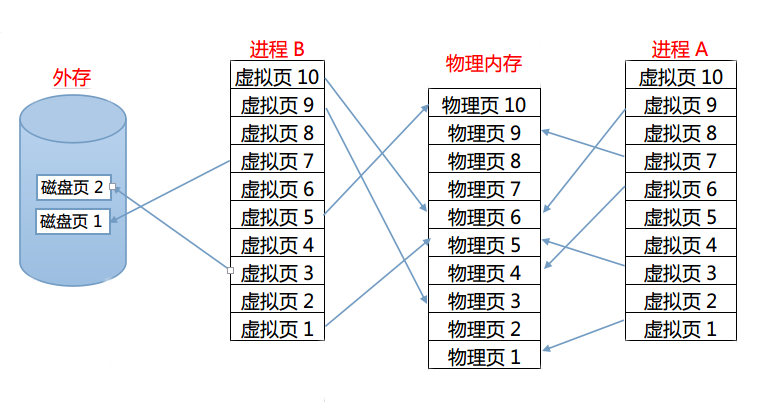
\includegraphics[scale=0.35]{picture/chapt9/PAGE_MAP.png}
      \caption{分页映射}
\end{figure}

\par 一图胜千言,我们看到了固定大小的物理页、虚拟页、甚至还有磁盘页。我觉得这张图片很能说明问题了,相信聪明的你从这里都悟出来了虚拟内存的实现原理了。没错,虚拟内存实质上就是把物理内存中暂时用不到的内容暂时换出到外存里,空出内存放置现阶段需要的数据。至于替换的策略当然有相应的算法了,比如最先换入原则,最少使用原则等等方法可以使用。

\par 相信通过上文的描述,我们对分页已经建立了初步的理解了。那么接下来的问题是,怎么表示和存储这个映射关系。这里描述起来简单,但是代码就不是那么直观了,原因很简单,因为需要一组数据结构来管理内存,但是这组数据结构本身也得放在内存里。所以牵扯到一个自己管理自己的问题。而且,开启分页模式之后,CPU立即就会按照分页模式的规则去解释线性地址了。所以,这意味着必须先建立好地址映射的数据结构,才能开启分页,而且必须保证之前的代码地址和数据地址都能映射正确。

\par 下面我们来说说x86下的一种简单的做法吧。

\par 在32位操作系统下使用32位地址总线(暂时原谅我在这里错误的描述吧,其实还有PAE这个东西),所以寻址空间有2的32次方,也就是4GB。一定要注意,我们强调了很多次了,这个空间里,有一些断断续续的地址实际上是指向了其它的外设,不过大部分还是指向RAM的。具体采取的分页大小可以有多种选择,但是过于小的分页会造成管理结构太大,过于大的分页又浪费内存。现在较为常见的分页是4KB一个页,也就是4096字节一个页。简单计算下,4GB的内存分成4KB一个的页,那就是1MB个页,没错吧?每个虚拟页到物理页的映射需要4个字节来存储的话(别忘了前提是32位环境下),整个4GB空间的映射需要4MB的数据结构来存储。

\par 目前看起来一切都很好,4MB似乎也不是很大。但是,这只是一个虚拟地址空间的映射啊,别忘了每个进程都有自己的映射,而且操作系统中通常有N个进程在运行。这样的话,假如有100个进程在运行,就需要400MB的内存来存储管理信息!这就太浪费了。

\par 怎么办?聪明的工程师们提出了分级页表的实现策略,他们提出了页目录,页表的概念。以32位的地址来说,分为3段来寻址,分别是地址的低12位,中间10位和高10位。高10位表示当前地址项在页目录中的偏移,最终偏移处指向对应的页表,中间10位是当前地址在该页表中的偏移,我们按照这个偏移就能查出来最终指向的物理页了,最低的12位表示当前地址在该物理页中的偏移。就这样,我们就实现了分级页表。

\par 我们来张图看看:

\begin{figure}[ht]
      \centering
      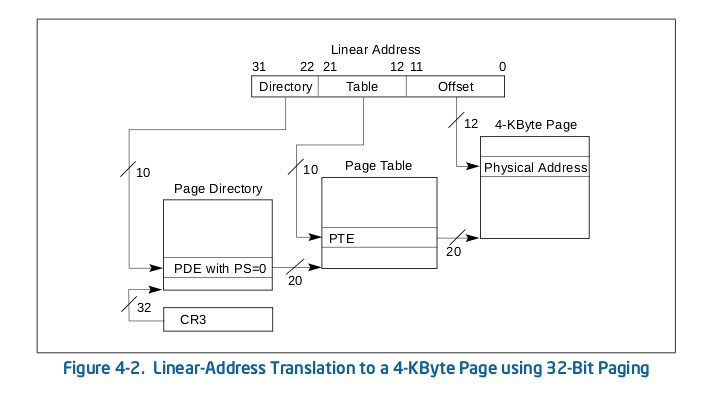
\includegraphics[scale=0.5]{picture/chapt9/PAGE.png}
      \caption{多级页表}
\end{figure}

\par 也许你已经算出来了,这样做的话映射4GB地址空间需要4MB+4KB的内存。我们这是搬起石头砸了自己的脚吗?当然不是,因为在一个进程中,实际使用到的内存大都远没有4GB这么大,所以通过两级页表的映射,我们就可以只映射需要的地址就可以了,是不是节省了内存呢?概念我们暂时就说到这里,更专业的描述和规范请参阅Intel文档,也就是上面那张图片的出处。

\par 说完了理论,接下来就是具体的实现了。我们把内存管理分为物理内存管理和虚拟内存管理两个部分来进行。本章讨论物理内存的管理。要实现内存的管理,首先要解决以下三个问题:

\begin{mdframed}
	\begin{enumerate}
		\item 如何获取可用物理内存的大小和地址?
		\item 采用什么样的数据结构来描述物理内存?
		\item 申请和释放物理内存的算法如何实现?
	\end{enumerate}
\end{mdframed}

\par 我们先来解决第一个问题。获取物理内存的方法一般有BIOS调用和直接探测等方法,但是GRUB的Mutliboot协议提供了更简单的方法。还记得那个multiboot\_t结构体吗?GRUB已经获取了物理内存的分布并且把它们放置在了这个结构体里的以下两个成员里。

\begin{lstlisting}[language = C, caption = include/multiboot.h]
typedef
struct multiboot_t {
	
	... ...

	/**
	 * 以下两项指出保存由 BIOS 提供的内存分布的缓冲区的地址和长度
	 * mmap_addr 是缓冲区的地址, mmap_length 是缓冲区的总大小
	 * 缓冲区由一个或者多个下面的 mmap_entry_t 组成
	 */
	uint32_t mmap_length;		
	uint32_t mmap_addr;
	
	... ...

} __attribute__((packed)) multiboot_t;

/**
 * size 是相关结构的大小,单位是字节,它可能大于最小值 20
 * base_addr_low 是启动地址的低32位,base_addr_high 是高 32 位,启动地址总共有 64 位
 * length_low 是内存区域大小的低32位,length_high 是内存区域大小的高 32 位,总共是 64 位
 * type 是相应地址区间的类型,1 代表可用 RAM,所有其它的值代表保留区域
 */
typedef
struct mmap_entry_t {
	uint32_t size; 		// size 是不含 size 自身变量的大小
	uint32_t base_addr_low;
	uint32_t base_addr_high;
	uint32_t length_low;
	uint32_t length_high;
	uint32_t type;
} __attribute__((packed)) mmap_entry_t;
\end{lstlisting}

\par GRUB将内存探测的结果按每个分段整理为mmap\_entry结构体的数组。mmap\_addr是这个结构体数组的首地址,mmap\_length是整个数组的长度。

\par 这里需要留意的是mmap\_entry结构体的size成员指的是除了size之外的成员的大小。至于base和length拆为了两段是因为物理地址可能用32位表示不下,不过我们只考虑32位操作系统,而且暂时只支持512MB的内存即可。type成员用来描述这个内存段的属性,因为物理不一定指向RAM里,也可能是其它外设。

\par 下面的代码实现了遍历这个结构,打印所有物理内存段的操作:

\begin{lstlisting}[language = C, caption = mm/pmm.c]
#include "multiboot.h"
#include "common.h"
#include "debug.h"
#include "pmm.h"

void show_memory_map()
{
	uint32_t mmap_addr = glb_mboot_ptr->mmap_addr;
	uint32_t mmap_length = glb_mboot_ptr->mmap_length;

	printk("Memory map:\n");

	mmap_entry_t *mmap = (mmap_entry_t *)mmap_addr;
	for (mmap = (mmap_entry_t *)mmap_addr; (uint32_t)mmap < mmap_addr + mmap_length; mmap++) {
		printk("base_addr = 0x%X%08X, length = 0x%X%08X, type = 0x%X\n",
			(uint32_t)mmap->base_addr_high, (uint32_t)mmap->base_addr_low,
			(uint32_t)mmap->length_high, (uint32_t)mmap->length_low,
			(uint32_t)mmap->type);
	}
}
\end{lstlisting}

\par 现在第一个问题解决了。等等,我们还需要知道内核本身加载到物理内存的位置信息,这块内存必须是物理内存管理所保留的。那怎么获取呢?看起来很困难,其实解决起来特别容易。大家想想,链接器负责了整个内核文件的链接和重定位工作,肯定知道内核文件加载到内存中的位置。我们修改链接器脚本,定义两个变量:

\begin{lstlisting}[caption = script/kernel.ld]
	... ...
	
	. = 0x100000;
	PROVIDE( kern_start = . );
	.text :
	{
		*(.text)
		. = ALIGN(4096);
	}

	... ....

	.stabstr :
	{
		*(.stabstr)
	 	. = ALIGN(4096);
	}
	PROVIDE( kern_end = . );
	
	... ...
\end{lstlisting}

\par 从上面的代码里可以看到最先放置的段.text的开始位置和最后一个段.stabstr的结尾分别定义了两个变量kern\_start和kern\_end,这两个变量在C代码里声明后就可以使用了。

\par 我们添加如下的头文件:

\begin{lstlisting}[language = C, caption = include/pmm.h]
#ifndef INCLUDE_PMM_H
#define INCLUDE_PMM_H

#include "multiboot.h"

// 内核文件在内存中的起始和结束位置
// 在链接器脚本中要求链接器定义
extern uint8_t kern_start[];
extern uint8_t kern_end[];

// 输出 BIOS 提供的物理内存布局
void show_memory_map();

#endif 	// INCLUDE_PMM_H
\end{lstlisting}

\par 接着修改入口函数进行测试,代码如下:

\begin{lstlisting}[language = C, caption = init/entry.c]
#include "console.h"
#include "debug.h"
#include "gdt.h"
#include "idt.h"
#include "timer.h"
#include "pmm.h"

int kern_entry()
{
	init_debug();
	init_gdt();
	init_idt();

	console_clear();
	printk_color(rc_black, rc_green, "Hello, OS kernel!\n\n");

	init_timer(200);

	// 开启中断
	// asm volatile ("sti");

	printk("kernel in memory start: 0x%08X\n", kern_start);
	printk("kernel in memory end:   0x%08X\n", kern_end);
	printk("kernel in memory used:   %d KB\n\n", (kern_end - kern_start + 1023) / 1024);
	
	show_memory_map();
	
	return 0;
}
\end{lstlisting}

\par 编译运行之后结果如下:

\begin{figure}[ht]
      \centering
      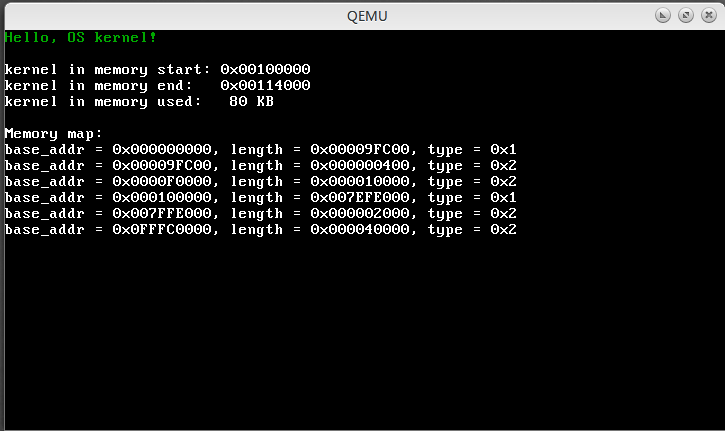
\includegraphics[scale=0.6]{picture/chapt9/PHY_MEM_MAP.png}
      \caption{物理内存布局}
\end{figure}

\par 我们采用的是qemu虚拟机默认的配置,所以物理内存大约是32MB。从这个输出结果中可以看到,可用的内存段是1MB以下的0x0-0x9FC00和1M以上的0x100000-0x7EFE000两段。需要注意的是这个区域随着我们的虚拟机内存设置不同而不同,所以这个值只是我自己虚拟机跑出来的一种结果。另外我们也成功的输出了内核的起始位置0x100000(1MB处)和结束位置0x114000以及占用的内存大小是80KB。\footnote{内核加载的结束位置和占用内存大小会随着代码和数据的逐渐增多而变大,这只是现阶段的大小。}

\par 第一个问题算是完全解决了,下面是第二个问题:采用什么样的数据结构来描述物理内存?

\par 为了支持后续的虚拟内存管理,物理内存也必须按照4KB的页框来管理内存。\footnote{这里的所谓的分页只是逻辑上的区分。}1MB以下的物理地址区域有太多的外设的存储区域映射在这里,为了大家实验的时候避免一些不必要的麻烦,我们不使用1MB以下的零碎物理内存,而是直接在1MB以上支持最多512MB的物理内存管理。

\par 物理内存管理算法最著名的就是Linux内核所采用的伙伴算法了,这方面的资料也很容易获取到。伙伴算法在申请和释放物理页框的时候会对物理页框进行合并操作,尽可能的保证可用物理内存的连续性。这里需要引入内存碎片这个概念,内存碎片分为内部碎片和外部碎片两种。内部碎片就是已经被分配出去却不能被利用的内存空间,比如我们为了管理方便,按照4KB内存块进行管理。此时任何申请内存的操作都会以4KB的倍数返回内存块。即使申请1个字节也返回指向4KB大的内存块的指针,这样的话造成了分配出去的内存没有被有效利用,而且剩余空间无法分配给其它进程(因为最小的管理单位是4KB)。外部碎片是指内存频繁请求和释放大小不同的连续页框后,导致在已分配页框块周围分散了许多小块空闲的页框,尽管这些空闲页框的总数可以满足接下来的请求,但却无法满足一个大块的连续页框。

\par 不过在本章并不会去实现伙伴算法。理由很简单,如果在大家对物理内存管理都没有概念的时候就贸然引入伙伴算法后带来的机制和策略的双重复杂性就难以学习和接受了。我们会采用一个很简单的策略来对内存进行管理操作:将物理页面的管理地址设定在1MB以上内核加载的结束位置之后,从这个起始位置到512MB的地址处,将所有的物理内存按页划分,将每页的地址放入栈里存储。这样在需要的时候就可以按页获取到物理内存了,具体的实现如下:

\begin{lstlisting}[language = C, caption = mm/pmm.c]
#include "multiboot.h"
#include "common.h"
#include "debug.h"
#include "pmm.h"

// 物理内存页面管理的栈
static uint32_t pmm_stack[PAGE_MAX_SIZE+1];

// 物理内存管理的栈指针
static uint32_t pmm_stack_top;

// 物理内存页的数量
uint32_t phy_page_count;

void show_memory_map()
{
	uint32_t mmap_addr = glb_mboot_ptr->mmap_addr;
	uint32_t mmap_length = glb_mboot_ptr->mmap_length;

	printk("Memory map:\n");

	mmap_entry_t *mmap = (mmap_entry_t *)mmap_addr;
	for (mmap = (mmap_entry_t *)mmap_addr; (uint32_t)mmap < mmap_addr + mmap_length; mmap++) {
		printk("base_addr = 0x%X%08X, length = 0x%X%08X, type = 0x%X\n",
			(uint32_t)mmap->base_addr_high, (uint32_t)mmap->base_addr_low,
			(uint32_t)mmap->length_high, (uint32_t)mmap->length_low,
			(uint32_t)mmap->type);
	}
}

void init_pmm()
{
	mmap_entry_t *mmap_start_addr = (mmap_entry_t *)glb_mboot_ptr->mmap_addr;
	mmap_entry_t *mmap_end_addr = (mmap_entry_t *)glb_mboot_ptr->mmap_addr + glb_mboot_ptr->mmap_length;

	mmap_entry_t *map_entry;

	for (map_entry = mmap_start_addr; map_entry < mmap_end_addr; map_entry++) {

		// 如果是可用内存 ( 按照协议,1 表示可用内存,其它数字指保留区域 )
		if (map_entry->type == 1 && map_entry->base_addr_low == 0x100000) {
			
			// 把内核结束位置到结束位置的内存段,按页存储到页管理栈里
			// 最多支持512MB的物理内存
			uint32_t page_addr = map_entry->base_addr_low + (uint32_t)(kern_end - kern_start);
			uint32_t length = map_entry->base_addr_low + map_entry->length_low;

			while (page_addr < length && page_addr <= PMM_MAX_SIZE) {
				pmm_free_page(page_addr);
				page_addr += PMM_PAGE_SIZE;
				phy_page_count++;
			}
		}
	}
}

uint32_t pmm_alloc_page()
{
	assert(pmm_stack_top != 0, "out of memory");

	uint32_t page = pmm_stack[pmm_stack_top--];

	return page;
}

void pmm_free_page(uint32_t p)
{
	assert(pmm_stack_top != PAGE_MAX_SIZE, "out of pmm_stack stack");

	pmm_stack[++pmm_stack_top] = p;
}
\end{lstlisting}

\par 其对应的头文件如下:

\begin{lstlisting}[language = C, caption = include/pmm.h]
#ifndef INCLUDE_PMM_H
#define INCLUDE_PMM_H

#include "multiboot.h"

// 线程栈的大小
#define STACK_SIZE 8192

// 支持的最大物理内存(512MB)
#define PMM_MAX_SIZE 0x20000000

// 物理内存页框大小 
#define PMM_PAGE_SIZE 0x1000

// 最多支持的物理页面个数
#define PAGE_MAX_SIZE (PMM_MAX_SIZE/PMM_PAGE_SIZE)

// 页掩码 按照 4096 对齐地址
#define PHY_PAGE_MASK 0xFFFFF000

// 内核文件在内存中的起始和结束位置
// 在链接器脚本中要求链接器定义
extern uint8_t kern_start[];
extern uint8_t kern_end[];

// 动态分配物理内存页的总数
extern uint32_t phy_page_count;

// 输出 BIOS 提供的物理内存布局
void show_memory_map();

// 初始化物理内存管理
void init_pmm();

// 返回一个内存页的物理地址
uint32_t pmm_alloc_page();

// 释放申请的内存
void pmm_free_page(uint32_t p);

#endif 	// INCLUDE_PMM_H
\end{lstlisting}

\par 最后修改入口函数为以下内容:

\begin{lstlisting}[language = C, caption = init/entry.c]
#include "console.h"
#include "debug.h"
#include "gdt.h"
#include "idt.h"
#include "timer.h"
#include "pmm.h"

int kern_entry()
{
	init_debug();
	init_gdt();
	init_idt();

	console_clear();
	printk_color(rc_black, rc_green, "Hello, OS kernel!\n");

	init_timer(200);
	
	// 开启中断
	// asm volatile ("sti");

	printk("kernel in memory start: 0x%08X\n", kern_start);
	printk("kernel in memory end:   0x%08X\n", kern_end);
	printk("kernel in memory used:   %d KB\n\n", (kern_end - kern_start) / 1024);
	
	show_memory_map();
	init_pmm();

	printk_color(rc_black, rc_red, "\nThe Count of Physical Memory Page is: %u\n\n", phy_page_count);

	uint32_t allc_addr = NULL;
	printk_color(rc_black, rc_light_brown, "Test Physical Memory Alloc :\n");
	allc_addr = pmm_alloc_page();
	printk_color(rc_black, rc_light_brown, "Alloc Physical Addr: 0x%08X\n", allc_addr);
	allc_addr = pmm_alloc_page();
	printk_color(rc_black, rc_light_brown, "Alloc Physical Addr: 0x%08X\n", allc_addr);
	allc_addr = pmm_alloc_page();
	printk_color(rc_black, rc_light_brown, "Alloc Physical Addr: 0x%08X\n", allc_addr);
	allc_addr = pmm_alloc_page();
	printk_color(rc_black, rc_light_brown, "Alloc Physical Addr: 0x%08X\n", allc_addr);

	return 0;
}
\end{lstlisting}

\par 最终的测试结果如图所示:

\begin{figure}[ht]
      \centering
      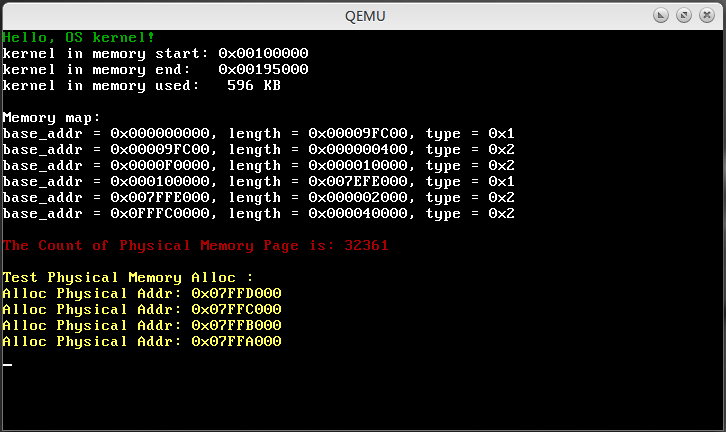
\includegraphics[scale=0.6]{picture/chapt9/PHY_MEM_ALLOC.png}
      \caption{原始的物理内存页分配函数}
\end{figure}


% 第10章
% -*- coding: UTF-8 -*-
% hurlex-chapt10.tex
% hurlex 开发文档 第10章内容

\section {虚拟内存管理的实现}

\par 这章将详细研讨虚拟内存管理的实现。

\par 上一章谈到,虚拟的页面每页占据4KB,按页为单位进行管理。物理内存也被分页管理,按照4KB分为一个个物理页框。虚拟地址到物理地址通过由页目录和页表组成的二级页表映射,页目录的地址放置在CR3寄存器里。

\par 至此,我们彻底揭开了x86下32位寻址的面纱,下图描述了地址转换的完整过程。

\begin{figure}[ht]
      \centering
      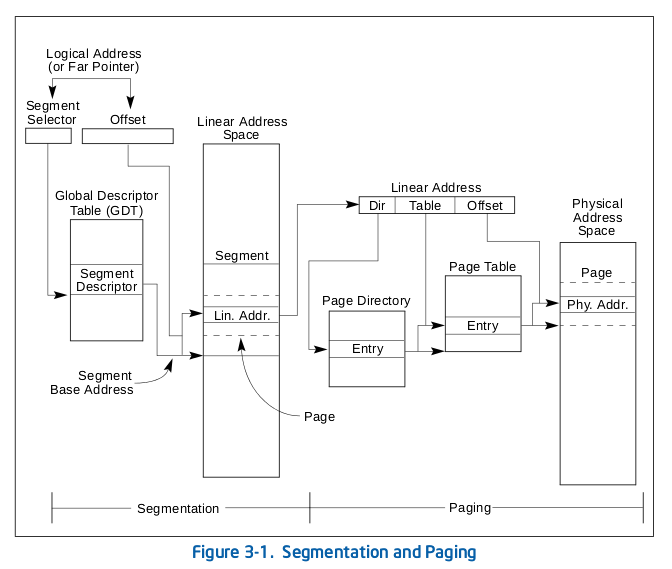
\includegraphics[scale=0.6]{picture/chapt10/ADDR_TRAN.png}
      \caption{段页式转换}
\end{figure}

\par 因为我们使用了Intel平坦模式的内存模型,所以之前的分段机制是被"绕过去"的,所以分页的管理就成了内存管理的核心了。首先是内核自身地址的映射,Linux采用的方案是把内核映射到线性地址空间3G以上,而应用程序占据线性地址空间0-3G的位置。我们的内核采取和Linux内核一样的映射,把物理地址0从虚拟地址0xC0000000(3G)处开始往上映射,因为我们只管理最多512MB的内存,所以3G-4G之间能完全的映射全部的物理地址。采取这个映射后,物理地址和内核虚拟地址满足以下关系:

\par 物理地址 + 0xC0000000 = 内核虚拟地址

\par 但是采用这个设计的话会给已有的代码带来什么麻烦呢?

\par 我们先引入VMA(Virtual Memory Address)和LMA(Load Memory Address)这两个概念。其中VMA是链接器生成可执行文件时的偏移计算地址,而LMA是区段所载入内存的实际地址。通常情况下的VMA是等于LMA的。使用以下命令可以查看内核文件的区段信息:
\begin{Verbatim}[frame=single]
    objdump -h hx_kernel
\end{Verbatim}

\par 输出大概是这个样子:

\begin{Verbatim}[frame=single]
hx_kernel:     file format elf32-i386

section:
Idx Name          Size      VMA       LMA       File off  Algn
  0 .text         00003000  00100000  00100000  00000080  2**4
                  CONTENTS, ALLOC, LOAD, READONLY, CODE
  1 .data         00001000  00103000  00103000  00003080  2**2
                  CONTENTS, ALLOC, LOAD, DATA
  2 .bss          00089c64  00104000  00104000  00004080  2**5
                  ALLOC
  3 .stab         0000539c  0018dc64  0018dc64  0008dce4  2**2
                  CONTENTS, ALLOC, LOAD, READONLY, DATA
  4 .stabstr      00002000  00193000  00193000  00093080  2**0
                  CONTENTS, ALLOC, LOAD, READONLY, DATA
\end{Verbatim}

\par 从上面的结果中能看到目前区段的加载地址和虚拟地址都是一样的。按照上面的设计,我们需要修改链接器脚本中各个段的起始位置。但是简单的把代码段的起始位置设为0xC0100000的话内核一运行就出错。为什么呢?因为GRUB是从1MB处加载内核的,而链接器是以0xC0100000这个参考地址进行地址重定位的。此时尚未开启虚拟页面映射,运行涉及到寻址的代码肯定就会出错。怎么办呢?看起来像是一个无解的死循环了。如果GRUB在加载内核之前就能设定好虚拟地址的映射再执行内核多好,或者有一段程序和数据按照0x100000的地址进行重定位,能帮助我们设置好一个临时的页表,再跳转到内核入口函数多好。前者貌似不可能实现,那后者呢?答案是肯定的,我们就采用这个方案。

\par GCC提供了这样的扩展机制:允许程序员指定某个函数或者某个变量所存储的区段。同时ld的链接脚本又可以自由定制,所以这个无解的问题就有了解决方案。用于设置这个临时页表和函数,我们指定它存储在.init段,只需要指定该段从0x100000地址开始,其他的.text和.data等段按照0xC0100000作为起始地址即可。当然这里还有要注意的细节,具体在下面的新链接脚本中可以看。因为代码变化比较大,所以贴出全部链接器脚本如下:

\begin{lstlisting}[caption = script/kernel.ld]
ENTRY(start)
SECTIONS
{
	PROVIDE( kern_start = 0xC0100000);
	. = 0x100000; 
	.init.text : 
	{
		*(.init.text)
		. = ALIGN(4096);
	}
	.init.data : 
	{
		*(.init.data)
		. = ALIGN(4096);
	}

	. += 0xC0000000;
	.text : AT(ADDR(.text) - 0xC0000000)
	{
		*(.text)
		. = ALIGN(4096);
	}
	.data : AT(ADDR(.data) - 0xC0000000)
	{
		*(.data)
		*(.rodata)
		. = ALIGN(4096);
	}
	.bss : AT(ADDR(.bss) - 0xC0000000)
	{
		*(.bss)
		. = ALIGN(4096);
	}
	.stab : AT(ADDR(.stab) - 0xC0000000)
	{
		*(.stab)
		. = ALIGN(4096);
	}
	.stabstr : AT(ADDR(.stabstr) - 0xC0000000)
	{
		*(.stabstr)
	 	. = ALIGN(4096);
	}
	PROVIDE( kern_end = . );
	
	/DISCARD/ : { *(.comment) *(.eh_frame) }
}
\end{lstlisting}

\par 链接脚本更新之后,之前一些代码也需要做出改动。首先要修改的是入口函数。因为修改的地方略多,所以贴出除声明外完整代码:

\begin{lstlisting}[language = {[x86masm]Assembler}, caption = boot/boot.s]
... ...

[BITS 32]  	; 所有代码以 32-bit 的方式编译

section .init.text 	; 临时代码段从这里开始

; 在代码段的起始位置设置符合 Multiboot 规范的标记

dd MBOOT_HEADER_MAGIC 	; GRUB 会通过这个魔数判断该映像是否支持
dd MBOOT_HEADER_FLAGS   ; GRUB 的一些加载时选项,其详细注释在定义处
dd MBOOT_CHECKSUM       ; 检测数值,其含义在定义处

[GLOBAL start] 		; 内核代码入口,此处提供该声明给 ld 链接器
[GLOBAL mboot_ptr_tmp] 	; 全局的 struct multiboot * 变量
[EXTERN kern_entry] 	; 声明内核 C 代码的入口函数

start:
	cli  				; 此时还没有设置好保护模式的中断处理
					; 所以必须关闭中断
	mov [mboot_ptr_tmp], ebx	; 将 ebx 中存储的指针存入 glb_mboot_ptr 变量
	mov esp, STACK_TOP  		; 设置内核栈地址,按照 multiboot 规范
	and esp, 0FFFFFFF0H		; 栈地址按照 16 字节对齐
	mov ebp, 0 			; 帧指针修改为 0
    
	call kern_entry	; 调用内核入口函数

;-----------------------------------------------------------------------------

section .init.data		; 开启分页前临时的数据段
stack:    times 1024 db 0  	; 这里作为临时内核栈
STACK_TOP equ $-stack-1 	; 内核栈顶,$ 符指代是当前地址

mboot_ptr_tmp: dd 0		; 全局的 multiboot 结构体指针

;-----------------------------------------------------------------------------
\end{lstlisting}

\par 主要的修改是第5行的代码所在段声明和第29行的数据所在段声明,因为此处代码和数据是在参考0x100000(1MB)编址的。所以在进入分页后需要更换新的内核栈和新的multiboot结构体指针。除此之外,仍就需要指定kern\_entry函数所在区段为.init.text段,并且在该函数中建立临时页表并跳转到高虚拟地址处的kern\_init函数正式执行,代码如下:

\begin{lstlisting}[language = C, caption = init/entry.c]
#include "console.h"
#include "string.h"
#include "debug.h"
#include "gdt.h"
#include "idt.h"
#include "timer.h"
#include "pmm.h"
#include "vmm.h"

// 内核初始化函数
void kern_init();

// 开启分页机制之后的 Multiboot 数据指针
multiboot_t *glb_mboot_ptr;

// 开启分页机制之后的内核栈
char kern_stack[STACK_SIZE];

// 内核使用的临时页表和页目录
// 该地址必须是页对齐的地址,内存 0-640KB 肯定是空闲的
__attribute__((section(".init.data"))) pgd_t *pgd_tmp  = (pgd_t *)0x1000;
__attribute__((section(".init.data"))) pgd_t *pte_low  = (pgd_t *)0x2000;
__attribute__((section(".init.data"))) pgd_t *pte_hign = (pgd_t *)0x3000;

// 内核入口函数
__attribute__((section(".init.text"))) void kern_entry()
{
	pgd_tmp[0] = (uint32_t)pte_low | PAGE_PRESENT | PAGE_WRITE;
	pgd_tmp[PGD_INDEX(PAGE_OFFSET)] = (uint32_t)pte_hign | PAGE_PRESENT | PAGE_WRITE;

	// 映射内核虚拟地址 4MB 到物理地址的前 4MB
	int i;
	for (i = 0; i < 1024; i++) {
		pte_low[i] = (i << 12) | PAGE_PRESENT | PAGE_WRITE;
	}

	// 映射 0x00000000-0x00400000 的物理地址到虚拟地址 0xC0000000-0xC0400000
	for (i = 0; i < 1024; i++) {
		pte_hign[i] = (i << 12) | PAGE_PRESENT | PAGE_WRITE;
	}
	
	// 设置临时页表
	asm volatile ("mov %0, %%cr3" : : "r" (pgd_tmp));

	uint32_t cr0;

	// 启用分页,将 cr0 寄存器的分页位置为 1 就好
	asm volatile ("mov %%cr0, %0" : "=r" (cr0));
	cr0 |= 0x80000000;
	asm volatile ("mov %0, %%cr0" : : "r" (cr0));
	
	// 切换内核栈
	uint32_t kern_stack_top = ((uint32_t)kern_stack + STACK_SIZE) & 0xFFFFFFF0;
	asm volatile ("mov %0, %%esp\n\t"
			"xor %%ebp, %%ebp" : : "r" (kern_stack_top));

	// 更新全局 multiboot_t 指针
	glb_mboot_ptr = mboot_ptr_tmp + PAGE_OFFSET;

	// 调用内核初始化函数
	kern_init();
}

void kern_init()
{
	init_debug();
	init_gdt();
	init_idt();

	console_clear();
	printk_color(rc_black, rc_green, "Hello, OS kernel!\n\n");

	init_timer(200);

	// 开启中断
	// asm volatile ("sti");

	printk("kernel in memory start: 0x%08X\n", kern_start);
	printk("kernel in memory end:   0x%08X\n", kern_end);
	printk("kernel in memory used:   %d KB\n\n", (kern_end - kern_start) / 1024);
	
	show_memory_map();
	init_pmm();

	printk_color(rc_black, rc_red, "\nThe Count of Physical Memory Page is: %u\n\n", phy_page_count);

	uint32_t allc_addr = NULL;
	printk_color(rc_black, rc_light_brown, "Test Physical Memory Alloc :\n");
	allc_addr = pmm_alloc_page();
	printk_color(rc_black, rc_light_brown, "Alloc Physical Addr: 0x%08X\n", allc_addr);
	allc_addr = pmm_alloc_page();
	printk_color(rc_black, rc_light_brown, "Alloc Physical Addr: 0x%08X\n", allc_addr);
	allc_addr = pmm_alloc_page();
	printk_color(rc_black, rc_light_brown, "Alloc Physical Addr: 0x%08X\n", allc_addr);
	allc_addr = pmm_alloc_page();
	printk_color(rc_black, rc_light_brown, "Alloc Physical Addr: 0x%08X\n", allc_addr);

	while (1) {
		asm volatile ("hlt");
	}
}
\end{lstlisting}

\par 代码中的 \_\_attribute\_\_((section(".init.data"))) 是GCC编译器的扩展功能,用来指定变量或者函数的存储区段。我们使用了1MB以下地址空间中的12KB来暂时放置临时页表。除此之外,入口函数中除了映射0xC0000000(3G)开始的4MB地址到物理内存0-4MB之外,我们依旧把虚拟地址的0-4MB映射到了物理地址的同样位置。为什么呢?因为在代码48-50行一旦将CR0寄存器最高位置为1的话,CPU立即就会进入分页机制去运行,此时所有的寻址都会按照分页机制的原则去进行,而kern\_entry函数本身是按照1MB起始地址生成的虚拟地址,如果不映射低端的虚拟地址的话,kern\_entry开启分页之后的代码访问就会出错。而最终离开了这个入口函数,进入内核初始化函数kern\_init的时候,已经处于高端虚拟地址的区域。所以在新的页表里不再需要低端的映射也可以正常寻址了。

\par 别忘了要更新multiboot.h的声明:

\begin{lstlisting}[language = C, caption = include/multiboot.h]
// 声明全局的 multiboot_t * 指针
// 内核未建立分页机制前暂存的指针
extern multiboot_t *mboot_ptr_tmp;

// 内核页表建立后的指针
extern multiboot_t *glb_mboot_ptr;

\end{lstlisting}

\par 另外还需要修改文本模式下显存的起始位置,原先的地址0xB8000此时需要加上偏移地址0xC0000000才可以在分页模式下正常访问到。

\begin{lstlisting}[language = C, caption = drivers/console.c]
... ...
// VGA 的显示缓冲的起点是 0xB8000
static uint16_t *video_memory = (uint16_t *)(0xB8000 + PAGE_OFFSET);
... ...
\end{lstlisting}

\par 之前的elf\_t结构体存储的是低端内存的地址,现在也必须加上页偏移:

\begin{lstlisting}[language = C, caption = kern/debug/elf.c]
... ...
// 从 multiboot_t 结构获取 ELF 信息
elf_t elf_from_multiboot(multiboot_t *mb)
{
	int i;
	elf_t elf;
	elf_section_header_t *sh = (elf_section_header_t *)mb->addr;

	uint32_t shstrtab = sh[mb->shndx].addr;
	for (i = 0; i < mb->num; i++) {
		const char *name = (const char *)(shstrtab + sh[i].name) + PAGE_OFFSET;
		// 在 GRUB 提供的 multiboot 信息中寻找内核 ELF 格式所提取的字符串表和符号表
		if (strcmp(name, ".strtab") == 0) {
			elf.strtab = (const char *)sh[i].addr + PAGE_OFFSET;
			elf.strtabsz = sh[i].size;
		}
		if (strcmp(name, ".symtab") == 0) {
			elf.symtab = (elf_symbol_t *)(sh[i].addr + PAGE_OFFSET);
			elf.symtabsz = sh[i].size;
		}
	}

	return elf;
}
... ...
\end{lstlisting}

\par 最后是实现虚拟内存管理的初始化了,这个函数将建立正式的内核页表并进行切换。同时还有进行地址映射和解除映射的函数实现:

\begin{lstlisting}[language = C, caption = mm/vmm.c]
#include "idt.h"
#include "string.h"
#include "debug.h"
#include "vmm.h"
#include "pmm.h"

// 内核页目录区域
pgd_t pgd_kern[PGD_SIZE] __attribute__ ((aligned(PAGE_SIZE)));

// 内核页表区域
static pte_t pte_kern[PTE_COUNT][PTE_SIZE] __attribute__ ((aligned(PAGE_SIZE)));

void init_vmm()
{
	// 0xC0000000 这个地址在页目录的索引
	uint32_t kern_pte_first_idx = PGD_INDEX(PAGE_OFFSET);
	
	uint32_t i, j;
	for (i = kern_pte_first_idx, j = 0; i < PTE_COUNT + kern_pte_first_idx; i++, j++) {
		// 此处是内核虚拟地址,MMU 需要物理地址,所以减去偏移,下同
		pgd_kern[i] = ((uint32_t)pte_kern[j] - PAGE_OFFSET) | PAGE_PRESENT | PAGE_WRITE;
	}

	uint32_t *pte = (uint32_t *)pte_kern;
	// 不映射第 0 页,便于跟踪 NULL 指针
	for (i = 1; i < PTE_COUNT * PTE_SIZE; i++) {
		pte[i] = (i << 12) | PAGE_PRESENT | PAGE_WRITE;
	}

	uint32_t pgd_kern_phy_addr = (uint32_t)pgd_kern - PAGE_OFFSET;

	// 注册页错误中断的处理函数 ( 14 是页故障的中断号 )
	register_interrupt_handler(14, &page_fault);

	switch_pgd(pgd_kern_phy_addr);
}

void switch_pgd(uint32_t pd)
{
	asm volatile ("mov %0, %%cr3" : : "r" (pd));
}

void map(pgd_t *pgd_now, uint32_t va, uint32_t pa, uint32_t flags)
{ 	
	uint32_t pgd_idx = PGD_INDEX(va);
	uint32_t pte_idx = PTE_INDEX(va); 
	
	pte_t *pte = (pte_t *)(pgd_now[pgd_idx] & PAGE_MASK);
	if (!pte) {
		pte = (pte_t *)pmm_alloc_page();
		pgd_now[pgd_idx] = (uint32_t)pte | PAGE_PRESENT | PAGE_WRITE;

		// 转换到内核线性地址并清 0
		pte = (pte_t *)((uint32_t)pte + PAGE_OFFSET);
		bzero(pte, PAGE_SIZE);
	} else {
		// 转换到内核线性地址
		pte = (pte_t *)((uint32_t)pte + PAGE_OFFSET);
	}

	pte[pte_idx] = (pa & PAGE_MASK) | flags;

	// 通知 CPU 更新页表缓存
	asm volatile ("invlpg (%0)" : : "a" (va));
}

void unmap(pgd_t *pgd_now, uint32_t va)
{
	uint32_t pgd_idx = PGD_INDEX(va);
	uint32_t pte_idx = PTE_INDEX(va);

	pte_t *pte = (pte_t *)(pgd_now[pgd_idx] & PAGE_MASK);

	if (!pte) {
		return;
	}

	// 转换到内核线性地址
	pte = (pte_t *)((uint32_t)pte + PAGE_OFFSET);

	pte[pte_idx] = 0;

	// 通知 CPU 更新页表缓存
	asm volatile ("invlpg (%0)" : : "a" (va));
}

uint32_t get_mapping(pgd_t *pgd_now, uint32_t va, uint32_t *pa)
{
	uint32_t pgd_idx = PGD_INDEX(va);
	uint32_t pte_idx = PTE_INDEX(va);

	pte_t *pte = (pte_t *)(pgd_now[pgd_idx] & PAGE_MASK);
	if (!pte) {
	      return 0;
	}
	
	// 转换到内核线性地址
	pte = (pte_t *)((uint32_t)pte + PAGE_OFFSET);

	// 如果地址有效而且指针不为NULL,则返回地址
	if (pte[pte_idx] != 0 && pa) {
		 *pa = pte[pte_idx] & PAGE_MASK;
		return 1;
	}

	return 0;
}
\end{lstlisting}

\par 需要注意的是Intel规定页表和页目录的起始位置必须是页对齐的,\_\_attribute\_\_ ((aligned(PAGE\_SIZE))) 是GCC的扩展指令,功能是使得变量的起始地址按照某个数值对齐,所以我们轻轻松松的就解决了这个难题。

\par 上面代码对应的头文件如下:

\begin{lstlisting}[language = C, caption = include/vmm.h]
#ifndef INCLUDE_VMM_H
#define INCLUDE_VMM_H

#include "types.h"
#include "idt.h"
#include "vmm.h"

// 内核的偏移地址
#define PAGE_OFFSET 	0xC0000000

/**
 * P-- 位 0 是存在 (Present) 标志,用于指明表项对地址转换是否有效。
 * P = 1 表示有效; P = 0 表示无效。
 * 在页转换过程中,如果说涉及的页目录或页表的表项无效,则会导致一个异常。
 * 如果 P = 0 ,那么除表示表项无效外,其余位可供程序自由使用。
 * 例如,操作系统可以使用这些位来保存已存储在磁盘上的页面的序号。
 */
#define PAGE_PRESENT 	0x1

/** 
 * R/W -- 位 1 是读 / 写 (Read/Write) 标志。如果等于 1 ,表示页面可以被读、写或执行。
 * 如果为 0 ,表示页面只读或可执行。
 * 当处理器运行在超级用户特权级 (级别 0,1 或 2) 时,则 R/W 位不起作用。
 * 页目录项中的 R/W 位对其所映射的所有页面起作用。
 */
#define PAGE_WRITE 	0x2

/**
 * U/S -- 位 2 是用户 / 超级用户 (User/Supervisor) 标志。
 * 如果为 1 ,那么运行在任何特权级上的程序都可以访问该页面。
 * 如果为 0 ,那么页面只能被运行在超级用户特权级 (0,1 或 2) 上的程序访问。
 * 页目录项中的 U/S 位对其所映射的所有页面起作用。
 */
#define PAGE_USER 	0x4

// 虚拟分页大小
#define PAGE_SIZE 	4096

// 页掩码,用于 4KB 对齐
#define PAGE_MASK      0xFFFFF000

// 获取一个地址的页目录项
#define PGD_INDEX(x) (((x) >> 22) & 0x3FF)

// 获取一个地址的页表项
#define PTE_INDEX(x) (((x) >> 12) & 0x3FF)

// 获取一个地址的页內偏移
#define OFFSET_INDEX(x) ((x) & 0xFFF)

// 页目录数据类型
typedef uint32_t pgd_t;

// 页表数据类型
typedef uint32_t pte_t;

// 页表成员数
#define PGD_SIZE (PAGE_SIZE/sizeof(pte_t))

// 页表成员数
#define PTE_SIZE (PAGE_SIZE/sizeof(uint32_t))

// 映射 512MB 内存所需要的页表数
#define PTE_COUNT 128

// 内核页目录区域
extern pgd_t pgd_kern[PGD_SIZE];

// 初始化虚拟内存管理
void init_vmm();

// 更换当前的页目录
void switch_pgd(uint32_t pd);

// 使用 flags 指出的页权限,把物理地址 pa 映射到虚拟地址 va
void map(pgd_t *pgd_now, uint32_t va, uint32_t pa, uint32_t flags);

// 取消虚拟地址 va 的物理映射
void unmap(pgd_t *pgd_now, uint32_t va);

// 如果虚拟地址 va 映射到物理地址则返回 1
// 同时如果 pa 不是空指针则把物理地址写入 pa 参数
uint32_t get_mapping(pgd_t *pgd_now, uint32_t va, uint32_t *pa);

// 页错误中断的函数处理
void page_fault(pt_regs *regs);

#endif 	// INCLUDE_VMM_H
\end{lstlisting}

\par 当CPU进入分页模式的时候,一旦发生内存访问的页错误,就会产生14号中断。上面注册的14号中断处理函数实现如下:

\begin{lstlisting}[language = C, caption = mm/page\_fault.c]
#include "vmm.h"
#include "debug.h"

void page_fault(pt_regs *regs)
{
	uint32_t cr2;
	asm volatile ("mov %%cr2, %0" : "=r" (cr2));

	printk("Page fault at 0x%x, virtual faulting address 0x%x\n", regs->eip, cr2);
	printk("Error code: %x\n", regs->err_code);

	// bit 0 为 0 指页面不存在内存里
	if ( !(regs->err_code & 0x1)) {
		printk_color(rc_black, rc_red, "Because the page wasn't present.\n");
	}
	// bit 1 为 0 表示读错误,为 1 为写错误
	if (regs->err_code & 0x2) {
		printk_color(rc_black, rc_red, "Write error.\n");
	} else {
		printk_color(rc_black, rc_red, "Read error.\n");
	}
	// bit 2 为 1 表示在用户模式打断的,为 0 是在内核模式打断的
	if (regs->err_code & 0x4) {
		printk_color(rc_black, rc_red, "In user mode.\n");
	} else {
		printk_color(rc_black, rc_red, "In kernel mode.\n");
	}
	// bit 3 为 1 表示错误是由保留位覆盖造成的
	if (regs->err_code & 0x8) {
		printk_color(rc_black, rc_red, "Reserved bits being overwritten.\n");
	}
	// bit 4 为 1 表示错误发生在取指令的时候
	if (regs->err_code & 0x10) {
		printk_color(rc_black, rc_red, "The fault occurred during an instruction fetch.\n");
	}

	while (1);
}
\end{lstlisting}

\par 整理好代码后进行编译,再用objdump查看可执行文件的段表,输出大致如下:

\begin{Verbatim}[frame=single]
hx_kernel:     file format elf32-i386

section:
Idx Name          Size      VMA       LMA       File off  Algn
  0 .init.text    00001000  00100000  00100000  00000094  2**0
                  CONTENTS, ALLOC, LOAD, READONLY, CODE
  1 .init.data    00001000  00101000  00101000  00001094  2**2
                  CONTENTS, ALLOC, LOAD, DATA
  2 .text         00003000  c0102000  00102000  00003000  2**4
                  CONTENTS, ALLOC, LOAD, READONLY, CODE
  3 .data         00001000  c0105000  00105000  00006000  2**2
                  CONTENTS, ALLOC, LOAD, DATA
  4 .bss          00105000  c0106000  00106000  00007000  2**12
                  ALLOC
  5 .stab         00005000  c020b000  0020b000  0010c000  2**2
                  CONTENTS, ALLOC, LOAD, READONLY, DATA
  6 .stabstr      00002000  c0210000  00210000  00111000  2**0
                  CONTENTS, ALLOC, LOAD, READONLY, DATA
\end{Verbatim}

\par 我们看到前两个区段和以前的输出类似,但是后面区段的VMA已经变成了加上了0xC0000000偏移的地址了。如果运行后能看到和上一章相同的输出结果就没有问题了。如果你得不到正确的结果,那就自己动手调试吧。


% 第11章
% -*- coding: UTF-8 -*-
% hurlex-chapt11.tex
% hurlex 开发文档 第11章内容

\section {内核堆管理的实现}

\par 前几章实现了内存的简单管理,但是目前的内存分配是按页为单位的,这样在需要分配小内存的时候比较容易造成内部碎片。这章我们来实现内核的堆管理算法,目的是为了小内存的分配。除了简单的分配内存之外,还需要考虑在内存释放的时候,对连续的内存进行合并。并且堆要实现在空闲内存过多的时候把物理页释放给物理内存管理模块。

\par 关于堆的实现有很多种,我们选择最简单的侵入式链表管理方法。如果你觉得可以胜任更好的算法完全可以自由发挥,而且之前的物理内存管理算法完全可以实现为伙伴系统。不过为了照顾大多数读者,我们选择简单的方式实现。当然,通过简单的算法熟悉了物理机制之后,完全可以抛开这些简单实现,去实现更好的算法。

\par 首先,在每一个申请的内存块之前插入一个描述当前内存块的结构体。结构体定义以及相关的函数声明如下:

\begin{lstlisting}[language = C, caption = include/heap.h]
#ifndef INCLUDE_HEAP_H_
#define INCLUDE_HEAP_H_

#include "types.h"

// 堆起始地址
#define HEAP_START 0xE0000000

// 内存块管理结构
typedef
struct header {
	struct header *prev; 	// 前后内存块管理结构指针
	struct header *next;
	uint32_t allocated : 1;	// 该内存块是否已经被申请
	uint32_t length : 31; 	// 当前内存块的长度
} header_t;

// 初始化堆
void init_heap();

// 内存申请
void *kmalloc(uint32_t len);

// 内存释放
void kfree(void *p);

// 测试内核堆申请释放
void test_heap();

#endif 	// INCLUDE_HEAP_H_
\end{lstlisting}

\par 结构体的定义里使用了C语言的位域定义,因为表示这块内存有没有被使用只需要1个bit就可以,这样节省内存。这里定义的堆的函数形式很简单,就不详细解释了。需要注意的是这里定义了虚拟堆起始地址为0xE0000000,它是内核页表没有使用的空闲区域。

\par 接下来是具体实现。除了以上的外部接口函数,还需要在实现文件里声明以下内部函数:

\begin{lstlisting}[language = C, caption = mm/heap.c]
#include "debug.h"
#include "pmm.h"
#include "vmm.h"
#include "heap.h"

// 申请内存块
static void alloc_chunk(uint32_t start, uint32_t len);

// 释放内存块
static void free_chunk(header_t *chunk);

// 切分内存块
static void split_chunk(header_t *chunk, uint32_t len);

// 合并内存块
static void glue_chunk(header_t *chunk);

static uint32_t heap_max = HEAP_START;

// 内存块管理头指针
static header_t *heap_first;
\end{lstlisting}

\par 这些内部函数只在堆的内部被调用,所以被声明为static,我们之前也强调过,不需要向外部暴露的函数最好用static限制其作用域。我们直接贴出相关函数的实现:

\begin{lstlisting}[language = C, caption = mm/heap.c]
... ...

void init_heap()
{
	heap_first = 0;
}

void *kmalloc(uint32_t len)
{
	// 所有申请的内存长度加上管理头的长度
	// 因为在内存申请和释放的时候要通过该结构去管理
	len += sizeof(header_t);

	header_t *cur_header = heap_first;
	header_t *prev_header = 0;

	while (cur_header) {
		// 如果当前内存块没有被申请过而且长度大于待申请的块
		if (cur_header->allocated == 0 && cur_header->length >= len) {
			// 按照当前长度切割内存
			split_chunk(cur_header, len);
			cur_header->allocated = 1;
			// 返回的时候必须将指针挪到管理结构之后
			return (void *)((uint32_t)cur_header + sizeof(header_t));
		}
		// 逐次推移指针
		prev_header = cur_header;
		cur_header = cur_header->next;
	}

	uint32_t chunk_start;

	// 第一次执行该函数则初始化内存块起始位置
	// 之后根据当前指针加上申请的长度即可
	if (prev_header) {
		chunk_start = (uint32_t)prev_header + prev_header->length;
	} else {
		chunk_start = HEAP_START;
		heap_first = (header_t *)chunk_start;
	}

	// 检查是否需要申请内存页
	alloc_chunk(chunk_start, len);
	cur_header = (header_t *)chunk_start;
	cur_header->prev = prev_header;
	cur_header->next = 0;
	cur_header->allocated = 1;
	cur_header->length = len;
	
	if (prev_header) {
		prev_header->next = cur_header;
	}

	return (void*)(chunk_start + sizeof(header_t));
}

void kfree(void *p)
{
	// 指针回退到管理结构,并将已使用标记置 0
	header_t *header = (header_t*)((uint32_t)p - sizeof(header_t));
	header->allocated = 0;

	// 粘合内存块
	glue_chunk(header);
}

void alloc_chunk(uint32_t start, uint32_t len)
{
	// 如果当前堆的位置已经到达界限则申请内存页
	// 必须循环申请内存页直到有到足够的可用内存
	while (start + len > heap_max) {
		uint32_t page = pmm_alloc_page();
		map(pgd_kern, heap_max, page, PAGE_PRESENT | PAGE_WRITE);
		heap_max += PAGE_SIZE;
	}
}

void free_chunk(header_t *chunk)
{
	if (chunk->prev == 0) {
		heap_first = 0;
	} else {
		chunk->prev->next = 0;
	}

	// 空闲的内存超过 1 页的话就释放掉
	while ((heap_max - PAGE_SIZE) >= (uint32_t)chunk) {
		heap_max -= PAGE_SIZE;
		uint32_t page;
		get_mapping(pgd_kern, heap_max, &page);
		unmap(pgd_kern, heap_max);
		pmm_free_page(page);
	}
}

void split_chunk(header_t *chunk, uint32_t len)
{
	// 切分内存块之前得保证之后的剩余内存至少容纳一个内存管理块的大小
	if (chunk->length - len > sizeof (header_t)) {
		header_t *newchunk = (header_t *)((uint32_t)chunk + chunk->length);
		newchunk->prev = chunk;
		newchunk->next = chunk->next;
		newchunk->allocated = 0;
		newchunk->length = chunk->length - len;

		chunk->next = newchunk;
		chunk->length = len;
	}
}

void glue_chunk(header_t *chunk)
{
	// 如果该内存块前面有链内存块且未被使用则拼合
	if (chunk->next && chunk->next->allocated == 0) {
		chunk->length = chunk->length + chunk->next->length;
		if (chunk->next->next) {
			chunk->next->next->prev = chunk;
		}
		chunk->next = chunk->next->next;
	}

	if (chunk->prev && chunk->prev->allocated == 0) {
		chunk->prev->length = chunk->prev->length + chunk->length;
		chunk->prev->next = chunk->next;
		if (chunk->next) {
			chunk->next->prev = chunk->prev;
		}
		chunk = chunk->prev;
	}

	// 假如该内存后面没有链表内存块了直接释放掉
	if (chunk->next == 0) {
		free_chunk(chunk);
	}
}
... ...
\end{lstlisting}

\par 这里的代码都很简单,只是链表的简单运用。需要注意的是映射和解除映射并释放的函数。如果理解起来有困难的话,建议你在调试模式下在纸上画一画,这样很容易理解。\footnote{这里的代码基本上来自James先生的实现,不过James先生的实现隐藏了比较多的BUG,我也是在纸上画过之后才找出的BUG。}

\par 最后添加一个简单的测试函数:

\begin{lstlisting}[language = C, caption = mm/heap.c]
void test_heap()
{
	printk_color(rc_black, rc_magenta, "Test kmalloc() && kfree() now ...\n\n");

	void *addr1 = kmalloc(50);
	printk("kmalloc    50 byte in 0x%X\n", addr1);
	void *addr2 = kmalloc(500);
	printk("kmalloc   500 byte in 0x%X\n", addr2);
	void *addr3 = kmalloc(5000);
	printk("kmalloc  5000 byte in 0x%X\n", addr3);
	void *addr4 = kmalloc(50000);
	printk("kmalloc 50000 byte in 0x%X\n\n", addr4);

	printk("free mem in 0x%X\n", addr1);
	kfree(addr1);
	printk("free mem in 0x%X\n", addr2);
	kfree(addr2);
	printk("free mem in 0x%X\n", addr3);
	kfree(addr3);
	printk("free mem in 0x%X\n\n", addr4);
	kfree(addr4);
}
\end{lstlisting}

\par 最后自然是测试了。在内核的初始化函数里加上堆的相关头文件并且调用初始化和测试函数,输出如下:

\begin{figure}[ht]
      \centering
      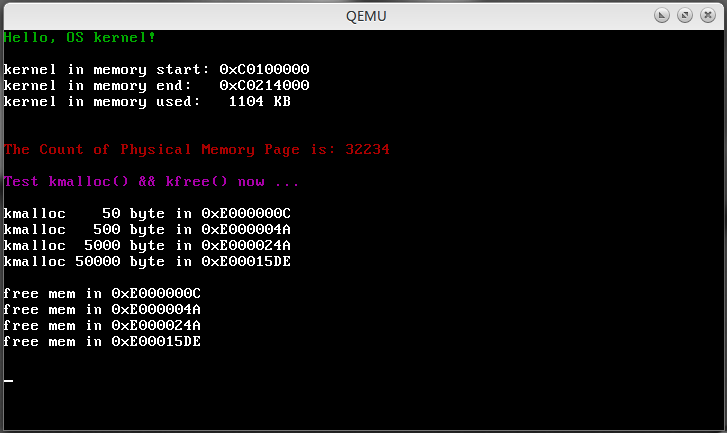
\includegraphics[scale=0.6]{picture/chapt11/HEAP_TEST.png}
      \caption{测试内核堆管理函数}
\end{figure}

\par OK,任务完成!

% 第12章
% -*- coding: UTF-8 -*-
% hurlex-chapt12.tex
% hurlex 开发文档 第12章内容

\section {内核线程的创建与切换}

\par 这一章我们将讨论内核线程的创建与切换。

\par 首先给出内核线程的含义,此处的内核线程作为运行在内核态的一个逻辑执行流,拥有私有的栈空间。但是除了这个私有的栈之外,不拥有其它的资源。所有的内核线程拥有相同的页表,共享所有的全局数据。

\par Intel的x86CPU提供任务切换机制是使用TSS段进行切换,这么做比较繁琐且效率较低,现代的OS都不会完全采用硬件切换机制。本章所阐述的任务切换只发生在内核态,不涉及特权级的转移过程,所以可以完全由硬件实现。而且这种实现用在用户级的线程库中亦可,大家有兴趣的话可以仿照这个思路实现用户级线程库。

\par 任务的切换必然涉及到现场的保护与恢复,所以就必然需要一个数据结构来保存这些现场信息。这个数据结构中一般也会放置任务相关的一些信息并且以链表之类的方式组织起来,这个结构被称之为PCB(Process Control Block)或者TCB(Task Control Block)。相关定义如下:

\begin{lstlisting}[language = C, caption = include/task.h]
#ifndef INCLUDE_TASK_H_
#define INCLUDE_TASK_H_

#include "types.h"
#include "pmm.h"
#include "vmm.h"

// 进程状态描述
typedef
enum task_state {
	TASK_UNINIT = 0, 	// 未初始化
	TASK_SLEEPING = 1, 	// 睡眠中
	TASK_RUNNABLE = 2, 	// 可运行(也许正在运行)
	TASK_ZOMBIE = 3, 	// 僵尸状态
} task_state;

// 内核线程的上下文切换保存的信息
struct context {
	uint32_t esp;
	uint32_t ebp;
	uint32_t ebx;
	uint32_t esi;
	uint32_t edi;
	uint32_t eflags;
};

// 进程内存地址结构
struct mm_struct {
	pgd_t *pgd_dir; 	// 进程页表
};

// 进程控制块 PCB 
struct task_struct {
	volatile task_state state; 	// 进程当前状态
	pid_t 	 pid; 			// 进程标识符
	void  	*stack; 		// 进程的内核栈地址
	struct mm_struct *mm; 		// 当前进程的内存地址映像
	struct context context; 	// 进程切换需要的上下文信息
	struct task_struct *next; 	// 链表指针
};

// 全局 pid 值
extern pid_t now_pid;

// 内核线程创建
int32_t kernel_thread(int (*fn)(void *), void *arg);

// 线程退出函数
void kthread_exit();

#endif 	// INCLUDE_TASK_H_
\end{lstlisting}

\par 除了描述每一个任务信息的结构,还需要将这些结构组织起来并且引入调度机制。相关的头文件和定义如下:

\begin{lstlisting}[language = C, caption = include/sched.h]
#ifndef INCLUDE_SCHEDULER_H_
#define INCLUDE_SCHEDULER_H_

#include "task.h"

// 可调度进程链表
extern struct task_struct *running_proc_head;

// 等待进程链表
extern struct task_struct *wait_proc_head;

// 当前运行的任务
extern struct task_struct *current;

// 初始化任务调度
void init_sched();

// 任务调度
void schedule();

// 任务切换准备
void change_task_to(struct task_struct *next);

// 任务切换
void switch_to(struct context *prev, struct context *next);

#endif 	// INCLUDE_SCHEDULER_H_
\end{lstlisting}

\par 本章不会采用复杂的调度策略,操作系统理论中各种调度算法都不会在这里实现。本章主要目的是说明白任务切换的原理。所以任务组织的方式就是一个单向循环链表,调度程序每次选择当前任务的下一个任务运行。如果你有兴趣,可以自己实现更好的调度算法。大家完全可以在PCB里增加新的数据成员,实现带有优先级的任务切换机制。

\par 在进行任务切换之前,内核原先的执行流还没有一个结构来保存其信息,所以需要在初始化调度之前给原始的执行流创建PCB信息。这里模仿Linux内核早期的做法,将PCB放置在线程栈的最低处。初始化的代码如下:

\begin{lstlisting}[language = C, caption = kernel/sched/sched.c]
#include "sched.h"
#include "heap.h"
#include "debug.h"

// 可调度进程链表
struct task_struct *running_proc_head = NULL;

// 等待进程链表
struct task_struct *wait_proc_head = NULL;

// 当前运行的任务
struct task_struct *current = NULL;

void init_sched()
{
	// 为当前执行流创建信息结构体 该结构位于当前执行流的栈最低端
	current = (struct task_struct *)(kern_stack_top - STACK_SIZE);

	current->state = TASK_RUNNABLE;
	current->pid = now_pid++;
	current->stack = current; 	// 该成员指向栈低地址
	current->mm = NULL; 		// 内核线程不需要该成员

	// 单向循环链表
	current->next = current;

	running_proc_head = current;
}
\end{lstlisting}

\par 调度函数很容易理解,每次都返回当前任务的下一个任务。代码如下:
\footnote{这里的调度函数留给大家自由发挥,去自由实现各种高端的调度算法。}

\begin{lstlisting}[language = C, caption = include/sched.h]
void schedule()
{
	if (current) {
		change_task_to(current->next);
	}
}

void change_task_to(struct task_struct *next)
{
	if (current != next) {
		struct task_struct *prev = current;
		current = next;
		switch_to(&(prev->context), &(current->context));
	}
}
\end{lstlisting}

\par 具体的切换操作由汇编实现,分别是保存当前任务的执行上下文和切换到下一个任务去。代码如下:

\begin{lstlisting}[language = {[x86masm]Assembler}, caption = kernel/sched/switch\_to.s]
[global switch_to]

; 具体的线程切换操作,重点在于寄存器的保存与恢复
switch_to:
        mov eax, [esp+4]

        mov [eax+0],  esp
        mov [eax+4],  ebp
        mov [eax+8],  ebx
        mov [eax+12], esi
        mov [eax+16], edi
        pushf
        pop ecx
        mov [eax+20], ecx

        mov eax, [esp+8]

        mov esp, [eax+0]
        mov ebp, [eax+4]
        mov ebx, [eax+8]
        mov esi, [eax+12]
        mov edi, [eax+16]
        mov eax, [eax+20]
        push eax
        popf
 	
        ret
\end{lstlisting}

\par 经过上面的铺垫,重头戏就是接下来的切换了。内核线程的创建和退出函数的实现如下:

\begin{lstlisting}[language = C, caption = include/task.h]
#include "gdt.h"
#include "pmm.h"
#include "vmm.h"
#include "heap.h"
#include "task.h"
#include "sched.h"
#include "string.h"
#include "debug.h"

// 全局 pid 值
pid_t now_pid = 0;

// 内核线程创建
int32_t kernel_thread(int (*fn)(void *), void *arg)
{
	struct task_struct *new_task = (struct task_struct *)kmalloc(STACK_SIZE);
	assert(new_task != NULL, "kern_thread: kmalloc error");

	// 将栈低端结构信息初始化为 0 
	bzero(new_task, sizeof(struct task_struct));

	new_task->state = TASK_RUNNABLE;
	new_task->stack = current;
	new_task->pid = now_pid++;
	new_task->mm = NULL;

	uint32_t *stack_top = (uint32_t *)((uint32_t)new_task + STACK_SIZE);

	*(--stack_top) = (uint32_t)arg;
	*(--stack_top) = (uint32_t)kthread_exit;
	*(--stack_top) = (uint32_t)fn;

	new_task->context.esp = (uint32_t)new_task + STACK_SIZE - sizeof(uint32_t) * 3;

	// 设置新任务的标志寄存器未屏蔽中断,很重要
	new_task->context.eflags = 0x200;
	new_task->next = running_proc_head;
	
	// 找到当前进任务队列,插入到末尾
	struct task_struct *tail = running_proc_head;
	assert(tail != NULL, "Must init sched!");

	while (tail->next != running_proc_head) {
		tail = tail->next;
	}
	tail->next = new_task;

	return new_task->pid;
}

void kthread_exit()
{
	register uint32_t val asm ("eax");

	printk("Thread exited with value %d\n", val);

	while (1);
}

\end{lstlisting}

\par 内核退出函数在这里只实现了简陋的一部分,标准做法是将退出线程的PCB结构转移到不可调度链表去,等待其他线程join后再清理结构。这个留给大家自由实现吧,可以自由发散思维去做。

\par 这里的内核线程的创建和切换过程可能有些晦涩,其切换的重点在于switch\_to函数最后的ret指令。在ret指令返回之前,由于之前的执行现场已经被切换,特别是esp指针指向的栈被切换了,所以ret指令弹出的返回地址自然就变成了另一个执行流之前调用任务切换函数之前保存的返回地址了。kernel\_thread函数便是通过构造出这样一个切换后可以弹出执行地址的初始栈来实现的。
\footnote{如果理解起来依旧有困难的话不妨在纸上画画调用栈,这样比较好理解。}

\par 解决了所有切换的问题之后,剩下的只是时间片的问题了。可能大家已经想到了,这个调度函数最终是要由timer中断函数来执行的。我们修改timer中断的处理函数如下:

\begin{lstlisting}[language = C, caption = drivers/timer.c]
void timer_callback(pt_regs *regs)
{
	schedule();
}
\end{lstlisting}

\par 在定时器初始化之后,我们开启INTR中断。此时timer中断会按照之前设定好的工作频率来执行调度任务。

\par 我们在初始化函数里测试下,代码如下:

\begin{lstlisting}[language = C, caption = init/entry.c]

... ...

int flag = 0;

int thread(void *arg)
{
	while (1) {
		if (flag == 1) {
			printk_color(rc_black, rc_green, "B");
			flag = 0;
		}
	}

	return 0;
}

void kern_init()
{
	init_debug();
	init_gdt();
	init_idt();

	console_clear();
	printk_color(rc_black, rc_green, "Hello, OS kernel!\n\n");

	init_timer(200);

	printk("kernel in memory start: 0x%08X\n", kern_start);
	printk("kernel in memory end:   0x%08X\n", kern_end);
	printk("kernel in memory used:   %d KB\n\n", (kern_end - kern_start) / 1024);
	
	// show_memory_map();
	init_pmm();
	init_vmm();
	init_heap();

	printk_color(rc_black, rc_red, "\nThe Count of Physical Memory Page is: %u\n\n", phy_page_count);
	test_heap();

	init_sched();

	kernel_thread(thread, NULL);

	// 开启中断
	enable_intr();

	while (1) {
		if (flag == 0) {
			printk_color(rc_black, rc_red, "A");
			flag = 1;
		}
	}

	while (1) {
		asm volatile ("hlt");
	}
}
\end{lstlisting}

\par 编译运行后,我们看到了完美交替输出的A和B,如图所示:

\begin{figure}[ht]
      \centering
      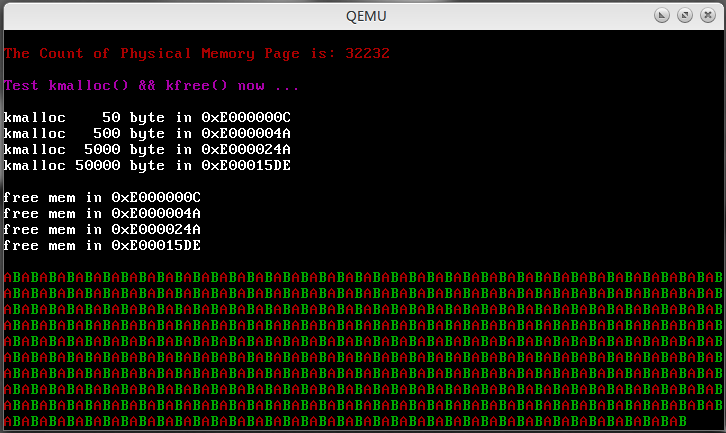
\includegraphics[scale=0.6]{picture/chapt12/KTHREAD.png}
      \caption{测试内核线程切换}
\end{figure}


% 第13章
% -*- coding: UTF-8 -*-
% hurlex-chapt13.tex
% hurlex 开发文档 第13章内容

\section {接下来如何继续学习}

\par 因为时间和精力的缘故,这篇教程到这里就趋于尾声了。可能大家原本期待的用户态的实现以及图形界面等等内容并没有看到,不免有所失望。但是我相信通过这篇教程,大家完全有能力根据其它的资料继续学习下去。下面我推荐一些书籍和论坛,有兴趣的话大家完全可以继续探索下去。

\par 首先是国内知名度较高的《Orange S:一个操作系统的实现》, 作者是于渊。虽然没有直接使用其中的任何代码,但我还是在参考文献里列出了这本书,因为它带我走入了操作系统实现的大门。

\par 接着还有一本《30天自制操作系统》,作者是川合秀实先生。这本书阐述的多是图形界面下的实现,但是因为作者剑走偏峰,而我主要是为了理解和掌握今年学习的本科操作系统课程而进行探索的,故没有参考这本书。

\par 最后推荐的是著名的OSDev论坛,这里有很不错的资料和讨论,每天看到国外的神人们在这里交谈和讨论也是一种很好的学习方法。论坛地址在教程最后的参考文献里,这里就不重复说了。

\par 另外国外很多大学都有相关的教学操作系统,比如麻省理工学院的的XV6,斯坦福的PintOS等等可以参考学习。相信有这篇教程的基础,大家能尽快理解这些相对来说较为复杂的系统。

\par 最后,感谢James先生的原始教程。如你所见,这里大多数代码来自James先生,尽管很多模块进行了重构和修改,但是很多代码依旧保持James先生的原貌,感谢他的慷慨和付出。

\par 这篇教程的代码继续以GPL V2协议发布,希望有助于更多的人学习和分享,感谢大家的阅读,谢谢。



% 列出所有的参考文献
\begin{thebibliography}{99}
	\bibitem {Jamesm} {JamesM's kernel development tutorials}, {http://www.jamesmolloy.co.uk/}
	\bibitem {OSDev} {OS Dev}, {http://wiki.osdev.org/}, {2011}
	\bibitem {IntelDoc} {Intel® 64 and IA-32 Architectures Software Developer’s Manual Volume3 : System Programming Guide},
		{Intel}, {1997-2003},
	\bibitem {x86Asm} {《x86 汇编语言 —— 从实模式到保护模式》}, {李忠 王晓波 余杰},
		 {电子工业出版社}, {2013}
	\bibitem {Orange} {《Orange S:一个操作系统的实现》}, {于渊}, {电子工业出版社}, {2009}
	\bibitem {x86PC} {《The x86 PC Assembly Language, Design and Interfacing》},
		{Muhammad Ali Mazidi、Janice Gillispie Mazidi、Danny Causey}, {电子工业出版社}, {2009}
	\bibitem {MOS} {《现代操作系统》}, {Andrew S. Tanenbaum}, {机械工业出版社}, {2012}
	\bibitem {IntelMP} {《Intel 微处理器》}, {Barry B.Brey}, {机械工业出版社}, {2008}
\end{thebibliography}

\end{document}

